\documentclass{article}

\usepackage{tikz}
\usepackage{lipsum}
\usepackage{graphicx}
\usepackage{subfigure}
\usepackage{enumitem}
\usepackage{tabu}
\usepackage{multirow}
\usepackage{amsmath}
\usepackage{amssymb}
\usepackage{epstopdf}
\usepackage{csquotes}
\usepackage{hyperref}
\usepackage{geometry}
%\usepackage[sorting=none, backend=biber, style=science]{biblatex} 
\usepackage[sorting=none, backend=biber]{biblatex} 
\usepackage{subcaption}
\usepackage{caption}
\usepackage{fancyhdr}
\usepackage[UKenglish]{babel}
\geometry{a4paper, portrait, margin=3cm}
\usepackage{duckuments}
\usepackage[export]{adjustbox}
\usepackage{setspace}
\usepackage{float}
\usepackage{mdframed}
%\usepackage{refcheck}

\onehalfspacing 

\graphicspath{ {src/figs/} }

%graphicx normal mode settings
\def\gridspace{20}
\def\doublegridspace{40}
\def\griddiagonal{10}
\def\griddot{\circle*{2}}

\setlength{\parskip}{0.5em}


%\DeclareCaptionFormat{customCaptionFormat}
%{ 
%    \textbf{#1#2}\text{\small#3}
%}
%\DeclareCaptionFont{phv}
%{
%    \fontseries{n}\fontfamily{phv}\selectfont
%}
\captionsetup{font=sf,labelfont=bf}

%Header and Footer Stuff

% \author{Jason Thomas}
% \date{October 2025}

% \fancypagestyle{plain}{%  the preset of fancyhdr 
%     \fancyhf{} % clear all header and footer fields
%     \fancyhead[C]{\thedate}
%     \fancyhead[L]{\theauthor}
    %\fancyhead[R]{\the}
% }
\pagestyle{plain}

\addbibresource{articleReferences.bib}

% For indenting all lists
\newcommand{\newandsetlength}[2]{\newlength{#1}\setlength{#1}{#2}}

\newandsetlength{\doubleparindent}{4cm}
\setlist[description]{leftmargin=\doubleparindent,labelindent=\parindent}

\definecolor{grey250}{RGB}{252,252,252}

% This is where your document will begin, after this anything you type should appear when compiled
\begin{document}

\begin{titlepage}
\begin{figure}[t!]
\centering

\includegraphics[width=5cm]{rmit-logo}
\end{figure}

\vspace*{2cm}

\begin{center}
{\large
	Probability of extinction for pathogens transmitted between ticks during co-feeding\\
	[1cm]
	A thesis submitted in fulfilment of the requirements for the degree of \\
    Bachelor of Science (Mathematics and Statistics) (Honours).\\
	[2cm]
	Jason Robert Thomas\\
	[0.5cm]
	Bachelor of Science (Mathematics and Statistics) \\
	[3cm]
	School of Science.\\
	[0.5cm]
	College of STEM.\\
	[0.5cm]
	RMIT University.\\
	[2cm]
	October 2025\\
}
\end{center}
	
\end{titlepage}

\section*{Declaration}
I certify that except where due acknowledgement has been made, the work is that of the author alone; the work has not been submitted previously, in whole or in part, to qualify for any other academic award; the content of the thesis is the result of work which has been carried out since the official commencement date of the approved research program; any editorial work, paid or unpaid, carried out by a third party is acknowledged; and, ethics procedures and guidelines have been followed. \\
[1cm]
Signed: Jason Thomas\\
[1cm]
Date: 29th of October, 2025\\

\section*{Acknowledgments}
I thank:
\begin{itemize}
\item Associate Professor Stephen Davis for his weekly supervision, feedback and advice during this project. Much of the content is based directly on Professor Davis' ideas.
\item Dr Haydar Demirhan and Dr Simon Robertson-Johnstone for their infrequent but valuable advice.
\item Daniel Longmuir, who helped me understand how to derive an important result.
\item Sarah Cowen, Cooper Maher and Amy Lambalk for proofreading. 
\end{itemize}

\section*{Statement of contribution}

All work presented in this thesis is my own, unless stated otherwise.

\thispagestyle{empty}
\addtocounter{page}{-1}

\newpage

\section*{Abstract}

Tick-borne pathogens cause significant health issues worldwide. Ticks feed on vertebrate hosts, which allows pathogens to spread and to cause harmful diseases. Pathogens sometimes infect ticks via co-feeding transmission, where a feeding tick transmits a pathogen directly to another co-feeding tick.

This project makes use of a branching process technique to determine the probability that a chain of co-feeding transmissions becomes extinct. We present a technique that we believe is novel to use commonly-collected tick burden data to find an offspring distribution, which is required to perform a branching process analysis. We use numerical techniques and simulations to find ranges of extinction probabilities.

This project uses 2004-2005 field data from the Kielder Forest in England, for hard-bodied tick species \textit{Ixodes ricinus} and \textit{Ixodes trianguliceps}, and two species of vertebrate host. We show that in some years in the Kielder Forest some pathogens would have a chance of persisting via co-feeding transmission alone.

This project uses a novel combination of Lorenz curves and a recent result for estimating $ R_0 $ in co-feeding transmission. For some combinations of tick and host species, just 1\% of vertebrate hosts are responsible for all co-feeding transmission potential.

\thispagestyle{empty}
\addtocounter{page}{-1}

\newpage

\section*{Graphical abstract}

\begin{figure}[h!]
	\begin{mdframed}[backgroundcolor=grey250,rightline=false,leftline=false,topline=false]
	    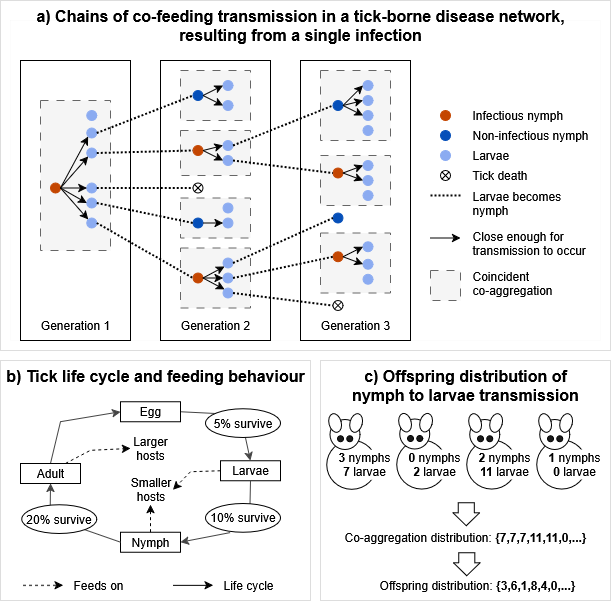
\includegraphics[width=0.99\textwidth, center]{graphical_abstract_mk2.drawio}
	    \caption{
	    \textbf{a)} \textit{Branching process}. Co-feeding transmission  occurs when susceptible ticks (usually larvae) attach and feed in close proximity to one or more infectious ticks (usually a nymph) and acquire a pathogen directly. This project introduces simplifying assumptions about the situation in nature: i) all larvae are susceptible; ii) larvae and nymphs might co-feed on one host, but they might not be close enough for transmission to occur; iii) there are no other routes of transmission; iv) two larvae that become infectious nymphs will not co-feed on the same vertebrate. \\ 
	    \textbf{b)} \textit{Life cycle}. This life cycle of ticks is: immature ticks are more plentiful, and that they tend to feed on small vertebrates \cite{Randolph1998}. This implies that immature ticks are largely responsible for co-feeding transmission. \\
	    \textbf{c)} \textit{Offspring distribution}. An offspring distribution is needed when using a branching process simulation. We use this simulation to calculate the probability that a chain of transmissions, starting with just a single infectious tick, goes extinct. We introduce a method to derive the offspring distribution from commonly-collected tick burden data.}
	    \label{fig:graphical_abstract}
	\end{mdframed}
\end{figure}

\thispagestyle{empty}
\addtocounter{page}{-1}

\newpage

\section*{Summary}

MAKE SHORTER 200 WORDS, MAKE IT NON-TECHNICAL

This thesis aims to predict the probability of extinction within a TBD network in a scenario where a single infectious nymph, a population of susceptible larvae, and a population of vertebrate hosts share a single habitat. To determine this probability, we find an offspring distribution and use a single-type GWBP, similar to the work by Lloyd-Smith et al \cite{LloydSmith2005}. However, where Lloyd-Smith et al used contact trace datasets for transmissions between people, we use field data that reports the larval and nymphal burdens (co-agggregation data) of vertebrate hosts that were collected in a survey at the Kielder Forest, in the United Kingdom, between 2004-2005 \cite{Bown2008, Bown2011}.

We introduce a novel technique to measure and compare the heterogeneity in vertebrates' ranked transmission potentials for facilitating co-feeding, without first having to obtain an estimate for $ R_0 $. This uses Lorenz curves and is inspired by the work of Perkins et al \cite{Perkins_2003} and Johnstone-Robertson et al \cite{JohnstoneRobertson2020}.

This thesis introduces what we believe is a novel method to obtain the parameters $ R_0 $ and $ k $ needed for an offspring distribution directly from the empirical co-aggregation data. In this project, we are unable to precisely determine $ R_0 $ for each subset of Kielder Forest data, so we report a range of possible probabilities of extinction. However, it might be feasible for other researchers to obtain accurate estimates for some particular combinations of tick species, host species and environmental conditions. We report threshold values that would allow $ R_0 > 1 $ for each subset of data.

To assist with understanding the probability of extinction within a TBD network, we re-implement many of the results by Lloyd-Smith et al. To find the parameters $ R_0 $ and $ k $, this project uses a reparameterised negative binomial distribution. We compare the goodness-of-fit for that distribution to the other distributions, and find that the negative binomial is either the best fit or close to the best in each case, which matches the findings of Lloyd-Smith et al. To help put many results in context, we re-implement and modify some simulations and visualisations made by Lloyd-Smith et al. 

To help more people use the results of this research, a link to all code used to generate the analysis and figures is provided in the Appendix. The Discussion addresses as many assumptions as possible, alternative assumptions, and the consequences of using those assumptions.

\thispagestyle{empty}
\addtocounter{page}{-1}

\newpage

\tableofcontents

\thispagestyle{empty}
\addtocounter{page}{-1}

\newpage

\section{Introduction}

Worldwide, tick-borne diseases (TBD) pose a significant health burden for humans and livestock. When ticks take blood meals from vertebrate hosts, pathogens living inside the ticks have an opportunity to infect the hosts. Those pathogens can cause diseases, with sometimes severe consequences for the individual vertebrate hosts that ticks feed on \cite{Johnson2023e}. This feeding behaviour allows for pathogens to spread either from tick-to-vertebrate-to-tick, or sometimes directly from tick-to-tick.

We can characterise and understand an individual tick's expected behaviour by its life stage. All tick species have four life stages: egg, larva, nymph and adult. During a tick's juvenile life stages - larvae then nymph - it will take blood meals from vertebrate hosts so that it can moult into its next life stage. Female adults will take a blood meal in order to produce eggs, but it will no longer moult \cite{Johnson2023a}.

When most ticks of a particular life stage feed on a small number of vertebrate hosts, then they are said to aggregate \cite{JohnstoneRobertson2020}. When ticks of different life stages aggregate, then this is known as co-aggregation. When those ticks co-aggregate at the same time, then this is known as coincident co-aggregation. Field data frequently shows that aggregation disproportionately affects only a fraction of the vertebrate host population, and the 80:20 rule is often cited for many parasites (including ticks), where 80\% of ticks can be found on just 20\% of vertebrate hosts \cite{Woolhouse1997}.

\subsection{Tick biology}

Ticks are in the \textit{Arachnida} class of animals, as are spiders and mites. Ticks are diverse and widespread; the diversity of ticks, and the vertebrate hosts that they feed on, is greater where the climate is more tropical, however, ticks are found on all continents except Antarctica \cite{Johnson2023a}. There are three families of ticks described in research: \textit{Ixodidae} (Hard Ticks), \textit{Argasidae} (Soft Ticks) and \textit{Nuttalliellidae}. \textit{Ixodidae} has the most known genuses and about 700 species. \textit{Nuttalliellidae} has just one known species \cite{Nicholson2019}.

A tick species' family is indicative of its behaviour. \textit{Ixodidae} ticks take a single blood meal during each life stage, whereas \textit{Argasidae} ticks take multiple blood meals during each life stage \cite{Johnson2023d}. Nidicolous ticks are said to spend their lives in burrows, caves and nests that their hosts live in. Many species are said to be specialists and will target few species of vertebrate hosts. Some nidicolous species of ticks are host-specific. Many species of \textit{Ixodidae} ticks are said to be non-nidicolous and their typical habitats include forests, meadows and other clearings, grasslands, savannahs, and semi-desert or desert areas. Such species are often said to be generalists, meaning they take blood meals from a wide array of hosts \cite{Nicholson2019}. Most \textit{Argasidae} are nidicolous \cite{Vial2009}, while only some \textit{Ixodidae} are nidicolous. 

This thesis will focus on species from the \textit{Ixodidae} family of ticks, which pose a more significant health concern for humans \cite{Parola2001}. Specifically, the analysis in this thesis will focus on \textit{Ixodes ricinus} and \textit{Ixodes trianguliceps}, for which we have data. \textit{I. ricinus} is said to be non-nidicolous while \textit{I. trianguliceps} is nidicolous \cite{Nicholson2019}.

The biology of \textit{Ixodidae} make them particularly competent vectors for many diseases. When they feed, they can stay attached for more than one week \cite{Johnson2023b}. Their extended period of feeding means that there is more time available for the transmission of pathogens \cite{Gray2024}. They lack digestive enzymes, meaning that their midgut is relatively benign, which increases the probability that a pathogen will survive inside the tick (this is defined later as transtadial transmission). When they feed, hard-bodied ticks inject saliva into their hosts, which increases the chance of successful transmission \cite{Gray2024}.

Usually the specialist Nidicolous ticks are not directly a threat to humans or livestock. Their sheltered lifestyle imposes limitations on their potential as vectors. The main role of nidicolous \textit{Ixodidae} ticks, in their relation to zoonotic diseases, appears to be the maintenance of pathogens in nature \cite{gray2014}. Non-nidicolous ticks, however, target a wider range of vertebrate hosts and therefore are more concerning from a public health policy perspective.

We can expect to find ticks of different life stages in differing frequencies. Ticks frequently die during and between their life stages, which implies larvae are most abundant, nymphs less common, and adults less common still \cite{Randolph1998}. A tick's life stage will also allow us to predict how it will feed. For \textit{I. ricinus}, adults tend to feed on larger vertebrate hosts, whereas immature \textit{I. ricinus} ticks will frequently feed on smaller vertebrate hosts \cite{Herrmann2015, Randolph1998}. In comparison, \textit{I. trianguliceps} will feed almost exclusively on small mammal hosts, and is regarded as a specialist \cite{Bown2003, Bown2008}.

\subsection{Tick-borne diseases}

Ticks harbour pathogens (viruses, bacteria and protozoa) that spread to vertebrate hosts when they take blood meals from those hosts. Those pathogens can cause diseases and many of those have severe health implications for vertebrate hosts, including humans \cite{Johnson2023e}.

\textit{I. ricinus} is the most important vector in central and western Europe; it is a vector for at least 20 pathogens, and at least eight pathogens that can affect humans, including Lyme disease and tick-borne encephalitis (TBE) \cite{Gray2024}. Pathogens transmitted by ticks are responsible for the majority of vector-borne disease in temperate North America, Europe and Asia, with Lyme Disease being the most prevalent tick-borne disease in the Northern Hemisphere \cite{Rochlin2020}. 

While the impact on human health is significant, so is the impact on the livestock industry. Research estimated that the estimated the global financial impact due to TBD was likely to be US\$22-30 billion per year \cite{Lew_Tabor_2016}. A 2006 article reported that economic losses in Tanzania's cattle industry were estimated to be \$364 million USD \cite{Kivaria2006}.

There are three ways that a pathogen can spread through populations of ticks, as Harrison and Bennett explain in their 2012 article:
\begin{itemize}
	\item \textit{Transovarial or vertical transmission:} Female ticks may transmit the pathogen to eggs.
	\item \textit{Systemic transmission:} Ticks may feed on, and infect, a host leading to the host's infection; other ticks may then acquire an infection by ingesting the infected host's blood.
	\item \textit{Co-feeding transmission:} Ticks may become infected by co-feeding alongside infected ticks; this does not require the host to have a systemic infection but instead pathogens are passed directly between ticks that feed in close proximity, and at the same time. \cite{HARRISON2012}.
\end{itemize}

In addition, for a tick-borne pathogen to survive in nature, it is necessary for ticks to transmit the pathogens onwards. However, that is not sufficient for the pathogen's survival. For a tick to become infected and then survive the moulting process to then pass on the disease, the pathogen first must survive transstadially; transstadial transmission is the tick's maintenance of the pathogen between life stages \cite{Johnson2023d}. This is a feature of systemic, vertical and co-feeding transmission.

The importance of different transmission routes depends on the tick and host species. Co-feeding transmission is important in TBD systems where vertebrate hosts are incompetent vectors for maintaining a pathogen \cite{HARRISON2012}. Several studies suggest that co-feeding transmission is required for TBE to persist in nature \cite{Hartemink2008, HARRISON2012}, but it is less important for the persistence of Lyme disease. Several studies on TBD show that co-feeding transmission will increase $ R_0 $, which is defined later in this introduction \cite{JohnstoneRobertson2020, Rosa2003, Norman2004}. Some studies show that co-feeding transmission may allow a pathogen to persist even without systemic transmission \cite{Rosa2003, Norman2004}. The focus of this thesis is on such a scenario.

If an \textit{Ixodidae} larva becomes infected during a blood meal (either via systemic or co-feeding transmission), then it becoming infectious is not guaranteed. It must first survive the moulting process to become a nymph. It must then find another vertebrate host to feed upon. If the pathogen survives transstadially, then further transmission is possible. For the species \textit{I. ricinus}, which is commonly called a deer tick or sheep tick, the larva-to-nymph moulting success rate was reported at 91.9\% under some laboratory conditions \cite{Hurry2021}. Research from 2016 suggested that larvae-to-nymph moulting success of \textit{I. ricinus} was dependent on environmental conditions, with evidence to suggest that snow cover would act as a temperature buffer during Germany's winter \cite{Dautel2016}. For the species \textit{I. trianguliceps}, mortality from larvae to nymph is density-dependent \cite{Randolph1994}. We note that, in trying to find the probability that an infected larva becomes an infectious tick, there is a lot of variation.

\subsection{Tick seasonal activity and distribution}

Ticks vary in their lifespans and yearly active periods, which imposes a seasonal constraint on the potential for co-feeding transmission to be of importance; if immature ticks feed at different times on the same vertebrate host, then co-feeding transmission will not occur. \textit{I. trianguliceps} has a lifespan of 2 to 5 years. All life stages seem to be active throughout the year but their activity peaks depending on where they live. In northern England, \textit{I trianguliceps} are most active in mid-autumn, while nymphal activity peaks in mid-summer, and infestations on rodents in the United Kingdom peak in summer and autumn \cite{Pf_ffle_2017}. \textit{I. ricinus} is also active in northern England. Their life cycle typically lasts between 2 and 3 years. \textit{I. ricinus} larvae activity frequently peaks in early summer while nymphal activity peaks in spring and autumn \cite{Otranto_2017}. Then for each species there is at least some expected overlap in their activity.

The geographical ranges of \textit{I. ricinus} and \textit{I. trianguliceps} often overlap. \textit{I. ricinus} has been reported in all parts of Europe, including Iceland, and throughout Northern Africa \cite{Otranto_2017}. \textit{I. trianguliceps} has been reported across mainland Europe and in the British Isles \cite{Pf_ffle_2017}. This thesis includes data from a single forest where \textit{I. ricinus} and \textit{I. trianguliceps} were collected from small mammals trapped during a longitudinal field study \cite{Bown2008, Bown2011}.

The habitat of \textit{I. ricinus} is expanding in Europe, due to several factors. \textit{I. ricinus} has increased its altitudinal range, based on studies in Bosnia and Herzegovina, the Czech Republic and Slovakia \cite{Medlock2013}. Modelling suggests that under different climate change scenarios, the habitat of \textit{I. ricinus} will probably spread northwards in Northern Europe \cite{Alkishe_2017}. Other modelling shows a similar northward spread of \textit{I. ricinus}, although some southern regions of Europe are likely to become less suitable for \textit{I. ricinus}, and some other species of ticks \cite{Cunze_2022}. However, the spread of \textit{I. ricinus} is not due to climate change alone; other drivers include the expansion of tick host populations, anthropogenic factors and land use changes \cite{Medlock2013}.

\subsection{The definition and importance of \texorpdfstring{$ R_0 $}{R0}}

The most important and widely-used concept in modelling transmissible diseases is the basic reproduction number $ R_0 $. This is a frequently-cited concept across epidemiology, and can be defined as the mean number of new infections per infection in an entirely susceptible population \cite{Diekman2000}.It differs from the effective reproductive number $ R_t $, which is used to quantify the efficacy of control measures in real time \cite{Lim2020}.

A consequence of using $ R_0 $, which is a notion of generational growth, is that it does not describe growth in real time. During the early stages of an outbreak in a susceptible population, we can understand growth as being exponential:

\begin{equation}
	I(t) \approx Ce^{rt} \nonumber
\end{equation}

where $ I $ is the total number of infections up until time $ t $, $ C $ is some constant, and $ r $ is the real time growth rate \cite{Diekman2000}.

$ R_0 $ is not a rate and is dimensionless, however, it has a relationship with the real-time growth rate, $ r $ \cite{Diekman2000}:

\begin{align}\label{R0}
  R_0 < 1 &\iff r < 0 \nonumber \\
  R_0 > 1 &\iff r > 0
\end{align}

In other words, the outbreak will undergo exponential decay when $ R_0 < 1 $, but an outbreak can be expected to persist when $ R_0 > 1 $. An important nuance is that $ R_0 > 1 $ is a necessary but insufficient condition for an outbreak to persist; due to stochasticity, the disease may still become extinct, even if $ R_0 > 1 $. This thesis will concentrate on $ R_0 $, rather than $ R_t $, because we assume that populations of ticks are entirely susceptible when a single infected tick is introduced.

Determining $ R_0 $ for wildlife disease systems often involves added complexities. Individual host species and individuals themselves have different susceptibilities, infectivity, and contacts. Given that an individual tick has different life stages, then these differences can exist within an individual throughout its life. Adding to the complexity is multiple transmission routes for many disease systems \cite{Hartemink2008}. Structured population models allow for modelling of these complexities \cite{Diekman2000}. However, this thesis investigates the particular case where only co-feeding transmission is possible. Therefore, $ R_0 $ in this thesis is simply the average number of new infections per infection. Finding $ R_0 $ in previous research has involved using contact trace data \cite{LloydSmith2005}, and this thesis introduces a method to simulate such data based on tick co-aggregation data.

\subsection{Heterogeneity in disease networks}

The extent to which individuals infected with transmissible diseases are able to infect their peers varies by multiple factors, including the specific disease, host population and environmental factors \cite{LloydSmith2005}. In transmissible disease systems, heterogeneity in individual behaviour can mean that some of the infected will not transmit the disease at all, while some might infect many of their peers.

An important notion to describe heterogeneity in disease systems is that of superspreading. Superspreading events are situations in which a few individuals are disproportionately responsible for infecting many others \cite{Galvani_2005}, which is often the case with infections like gonohrea and HIV/AIDS. The individuals who transmit the disease in these situations are superspreaders. Important research in 2005 made the case that superspreading events are normal events in the spread of infectious diseases \cite{LloydSmith2005}, and that work included a method to predict the frequency of superspreading events. Prior to 2005, there was already evidence of superspreading in disease networks. Data from the early-2000s SARS epidemic in Singapore showed that five individuals were identified as superspreaders after infecting another 103 individuals \cite{CDC2003}.

Superspreading is not just a feature of pathogens transmitted between humans; pathogens transmitted between other animals can exhibit the same behaviour, and there are multiple ways for superspreading to occur within those transmission networks. While it is true that some infected individuals will come into contact with more of their peers, and are in a sense superspreaders, it is also true that some individuals have a higher infectiousness and are "super-sheaders" \cite{VanderWaal_2016}. We can expect both of these types of heterogeneity (in contact and transmission) to be present in TBD systems.

For an individual tick to infect many others, a necessary but insufficient condition is co-incident co-aggregation \cite{Ferreri2014}, which we previously defined as the simultaneous aggregation of ticks from different life stages. Levels of aggregation are an indicator for, and pose a limit on, co-incident co-aggregation. To understand the heterogeneity in tick aggregation, the 80:20 rule is often cited. This is where 80\% of cases are caused by 20\% of infected individuals. Many vector-borne and sexually-transmitted diseases follow the 80:20 rule \cite{Woolhouse1997}. This heterogeneity is also present in TBD systems where there is significant evidence to suggest that aggregation data follows the 80:20 rule \cite{Ferreri2014, Brunner2008, JohnstoneRobertson2020}.

An interesting result in 2003 showed that when co-feeding ticks were considered, the transmission potential of the most-infested vertebrate hosts was even larger. Perkins et al used Lorenz curves to quantify the heterogeneity in transmission potentials by ranking the most-tick infested vertebrate hosts. They found that 20\% of vertebrate hosts were responsible for 74\% of transmission potential, but that proportion jumped to 94\% when only co-feeding ticks were considered \cite{Perkins_2003}. This project takes inspiration from the work by Perkins et al and will also use Lorenz curves to quantify transmission potential for co-feeding, but will use a different calculation.

The heterogeneity that is present in many transmission networks affects the choice of models we may choose to employ. Classically, models of disease outbreaks have assumed homogeneity in individual infectiousness and behaviour \cite{Garske2008}. These have typically been compartment models; the Susceptible-Infectious-Recovered systems of ordinary differential equations are common, although they can take many forms with more compartments defined. An assumption of those models is that the compartments are each large enough that the behaviour of individuals in those compartments are homogeneous. That is an appropriate assumption once an outbreak is established. However, at the start of an outbreak the number of infectious individuals must be small. This exposes a limitation: compartment models that lack a stochastic element are insufficient to describe the very early stages of an outbreak \cite{Brauer2008a}. Also in any population, the degree of infectiousness is distributed continuously, which further impedes our ability to divide a population into homogeneous subgroups \cite{LloydSmith2005}. One approach is to use the SIR modelling framework to define stochastic differential equations \cite{Allen2017}, but there are other stochastic methods available. This thesis addresses the heterogeneity that occurs in TBD systems by using a branching process simulation, which is defined in a later section of this introduction.

\subsection{Using the negative binomial distribution}

The work of Lloyd-Smith and others in 2005 showed that the negative binomial distribution was a better fit than either the Poisson or geometric distributions to many contact trace and surveillance datasets \cite{LloydSmith2005}; this is an important result that this thesis will reproduce. While the negative binomial distribution is frequently presented in textbooks with an integer parameter, Lloyd-Smith et al used a reparameterisation that allows for two continuous parameters: sample mean $ m $ and dispersion parameter, although that was a known result $ k $ \cite{Rice2007}. For a contact trace dataset, the sample mean is $ R_0 $. Lloyd-Smith et al showed that $ R_0 $ can be low and a pathogen may still spread if the over-dispersion parameter $ k $ is low enough, since a low $ k $ indicates heterogeneity in the data, meaning there are superspreading events that allow a transmissible pathogen to spread.

The work by Lloyd-Smith et al introduced the notion of an individual reproductive number $ v $, which represents individuals' variation in disease history. They represented this as a Gamma-distributed random variable and used that in a Poisson mixture to derive a negative binomial distribution, as below:

\begin{align}\label{PoissonMixture}
	v &\sim \text{Gamma}\left(R_0, \frac{R_0}{k}\right) \nonumber \\
	Z &\sim \text{Poisson}(v) \\
	Z &\sim \text{negbinom}(R_0, k) \nonumber
\end{align}

This is useful for several reasons. It allows us to query the effect of individual heterogeneity, and Lloyd-Smith et al found systems with high individual variation had infrequent but explosive outbreaks. This is a useful result because it allows for estimating the probability that a chain of transmission becomes extinct via numerical approximation, which is explored later in this project.

The negative binomial distribution is also important in modelling TBD systems. It has become the de facto choice for tick aggregation data, and for parasite aggregation data more generally. In 1998, Shaw et al showed that the NB distribution was an appropriate fit for 90\% of aggregation datasets that they looked at \cite{SHAW1998}. Many articles concerning tick aggregation data have used the negative binomial distribution \cite{Bown2003, HARRISON2012, Brunner2008}. Other work suggests that when tick aggregation data has a heavy right tail, which indicates extreme heterogeneity in vectors on hosts, then the Power-Law distribution is a better fit for some purposes \cite{Ferreri2014, Bisanzio2010}.

\subsection{Thinking about TBD transmission using contact networks}

Contact networks are a frequently-used tool in the analysis of how pathogens spread. Contact networks are graphs where vertices represent individuals and edges between them represent contacts. Those contacts may also facilitate transmission; the edges and nodes of a transmission network are contained within a contact network. 

Network thinking can help overcome some of the problems associated with deterministic compartment models; network models allow for representing the heterogeneity that exists in individual behaviour, and superspreaders can be represented as nodes with many outgoing edges. Network approaches can lead to useful outcomes, as some simulations suggest that stochastic methods lead to more accurate estimates for $ R_0 $ when early outbreak data is used \cite{Brauer2008b}.

In 2010, Bisanzio et al modelled the potential spread of TBE and Lyme disease. Their analysis focused on co-aggregation data for \textit{I. ricinus}. They made a bipartite contact network to represent the potential for transmission between vectors and hosts. Their analysis, which used bipartite networks to represent contacts between vector and host, showed that extreme aggregation on hosts would greatly impact the epidemic threshold \cite{Bisanzio2010}. Their work showed some evidence of the power law distribution is a better fit than the negative binomial distribution for the right tail of aggregation on hosts. In 2016, the work of Ferreri et al followed the work of Bisanzio et al. Their model represented aggregation as star graphs, with vertebrates at the centre and ticks as peripheral nodes. Their analysis focused on co-feeding transmission, but the model did not differentiate between the different life stages of ticks \cite{ferreri2016}.

In 2020, the work of Johnstone-Robertsone et al characterised a tick-host contact network as a directed, acyclic, bipartite graph. The ticks represent one node, but the edges leading away from the vertebrate host node $ k_{out} $ represent the number of larvae that co-aggregate, and $ k_{in} $ represent the number of nymphs that co-aggregate. However, there is only one node per tick. This implies that the tick nodes represent a tick in its larval and then nymphal life stages. Johnstone-Robertson et al then superimposed a transmission network that featured co-feeding transmission (edges between ticks) and systemic transmission (edges from tick-to-host, host-to-tick) \cite{JohnstoneRobertson2020}. This work is the main inspiration for the method, which is presented later in this thesis, of simulating outbreaks by using co-aggregation data. An important result in the Johnstone-Robertson paper is that for co-feeding transmission

\begin{equation} \label{JohnstoneRobertsonR0Estimate}
	R_0 \propto \frac{\langle k_{in}k_{out} \rangle}{\langle k_{in} \rangle } 
\end{equation}

where $ k_{in} $ is the number of nymphs and $ k_{out} $ is the number of larvae that are found on an individual vertebrate host. This result is also used to quantify the heterogeneity that exists in co-aggregation data.

\subsection{Galton-Watson Branching Processes}

A Galton-Watson Branching Process (GWBP) is a useful device for analysing how a disease spreads, but its original use was concerned with the extinction of families in Victorian Britain \cite{Athreya1972}. Whether a family becomes extinct because each father has no sons to carry on the family name, or a disease outbreak becomes extinct because each infected individual infects no one else, are addressed with the same technique.

A single-type GWBP branching process is such that all offspring, in all generations, belong to the same category; for a TBD, that could mean a specific species, particular life stage or infected by a particular pathogen. GWBP are also discrete-time Markov chains; the number of offspring in generation $ n $ depends on the probability of extinction in generation $ n - 1 $, but not on previous generations \cite{Allen2019}.

A requirement for using any branching process simulation is to define an offspring distribution. This is a discrete random variable that represents the number of new infections per infection (or sons per father, or new cells per cell, and so on). Let $ q_k $ be the offspring distribution, such that $ \sum_{k=0}^\infty q_k = 1 $ \cite{Diekman2000}, where $ k $ is the number of offspring.  Note that if $ q_k $ is known, then we can determine $ R_0 $:

\begin{equation}\label{offspringR0}
	R_0 = \sum_{k=1}^\infty k q_k
\end{equation}

For a single-type GWBP, let $ z $ be the probability of extinction, and note that $ g(z) $ is a probability generating function. $ z $ is applied to individuals in the branching process in the sense that for extinction to occur, every individual must have $ 0 $ offspring.

\begin{equation}\label{BranchingProcessPGF}
    g(z) = \sum_{k=0}^\infty q_k z^k, |z| < 1
\end{equation}

The intuition for the $ z^k $ term is if there are $ k $ individuals then the probability $ z $ must be considered $ k $ times, since we require all individuals at that point to have no offspring.

Now, let $ z_n $ be the probability that the chain is extinct after $ n $ generations. Then substitute $ z_n = g(z_{n-1})$

\begin{equation}\label{BranchingProcessRecurrence}
    z_{n} = g(z_{n-1}) = \sum_{k=0}^\infty q_k (z_{n-1})^k
\end{equation}

Note this has the Markov property, since the probability of extinction for generation $ n $ only relies on generation $ n-1 $.

This indicates $ z_n $ increases monotonically. But since all $ |z_n| \le 1 $, then this series converges, which leads to the simplification $ z = g(z) $. Thanks to that simplification, we find that the function is equal to its independent variable, and that means we can find an approximation for it via fixed point iteration. While that result is useful, we can avoid the calculation when extinction is guaranteed.: since $ R_0 $ is known \eqref{offspringR0}, then we can use $ R_0 \le 1 \implies z_{\infty} = 1 $ \cite{Diekman2000}.

The single-type branching process defined above is useful when offspring are the same type as their parent \cite{Allen2019}. However, many disease systems can be modelled using a multi-type branching process, which are capable of representing more complex systems that have more than just one pathogen, multiple species of host, and ticks in multiple different life-stages.

Multi-type GWBP simulations have been used to model TBD previously, which have effectively addressed the small number of infected individuals that limits the use of deterministic compartment models. In one article on TBD, authors compared predictions made using a deterministic compartment model and a multi-type GWBP to represent systemic transmission between hosts and vectors. They found the deterministic model would predict a stable endemic equilibrium if $ R_0 > 1 $, whereas the stochastic models would sometimes still lead to disease extinction even if $ R_0 > 1 $ \cite{Maliyoni_2017}. 

In this thesis, we model transmission as infectious nymphs beget new infectious nymphs during co-feeding. Furthermore, this project assumes that the tick species are not competent vectors for the same pathogens and that the vertebrate hosts have different behaviours. We also note different larval and nymphal activity for both tick species varies by year. So, we use a single-type GWBP for each combination of tick species, host species and year.

\newpage

\section{Summaries of Kielder Forest data}

This project makes use of data provided by **INSERT** Kevin Bown. The **INSERT** collected that data in the Kielder Forest in the United Kingdom between April and August in 2004 and 2005. The provided dataset presents the numbers of larvae and nymphs found on each vertebrate. Vertebrates were included in the collection once only.

The analysis by Bown et al originally **INSERT DETAILS ABOUT WHY THEY COLLECTED THE DATA, HOW, ETC**.

The data includes only the tick species \textit{I. trianguliceps} and  \textit{I. ricinus}. The host species were mostly "field voles", (\textit{Microtus agrestis}), and "common shrews" (\textit{Sorex araneus}). The researchers also encountered small numbers of other small mammals. The common shrew and field voles vastly outnumber other vertebrate hosts in the Kielder Forest data. The use of that data in this project focuses on the common shrew and field vole observations. 

\subsection{Evidence of co-aggregation}

Of interest is whether larvae and nymphs of a particular tick species have the same seasonal variation in activity. If the larvae and nymphs are active at different times, then the opportunity for co-feeding transmission to occur is limited. Seasonal activity for nymphs and larvae, for \textit{I. ricinus} and \textit{I. trianguliceps}, collected at the Kielder Forest is presented in Figure \ref{fig:kielder_seasonal}.

\begin{figure}[]
	\begin{mdframed}[backgroundcolor=grey250,rightline=false,leftline=false,topline=false]
	\centering
	\begin{tabular}{ll}
		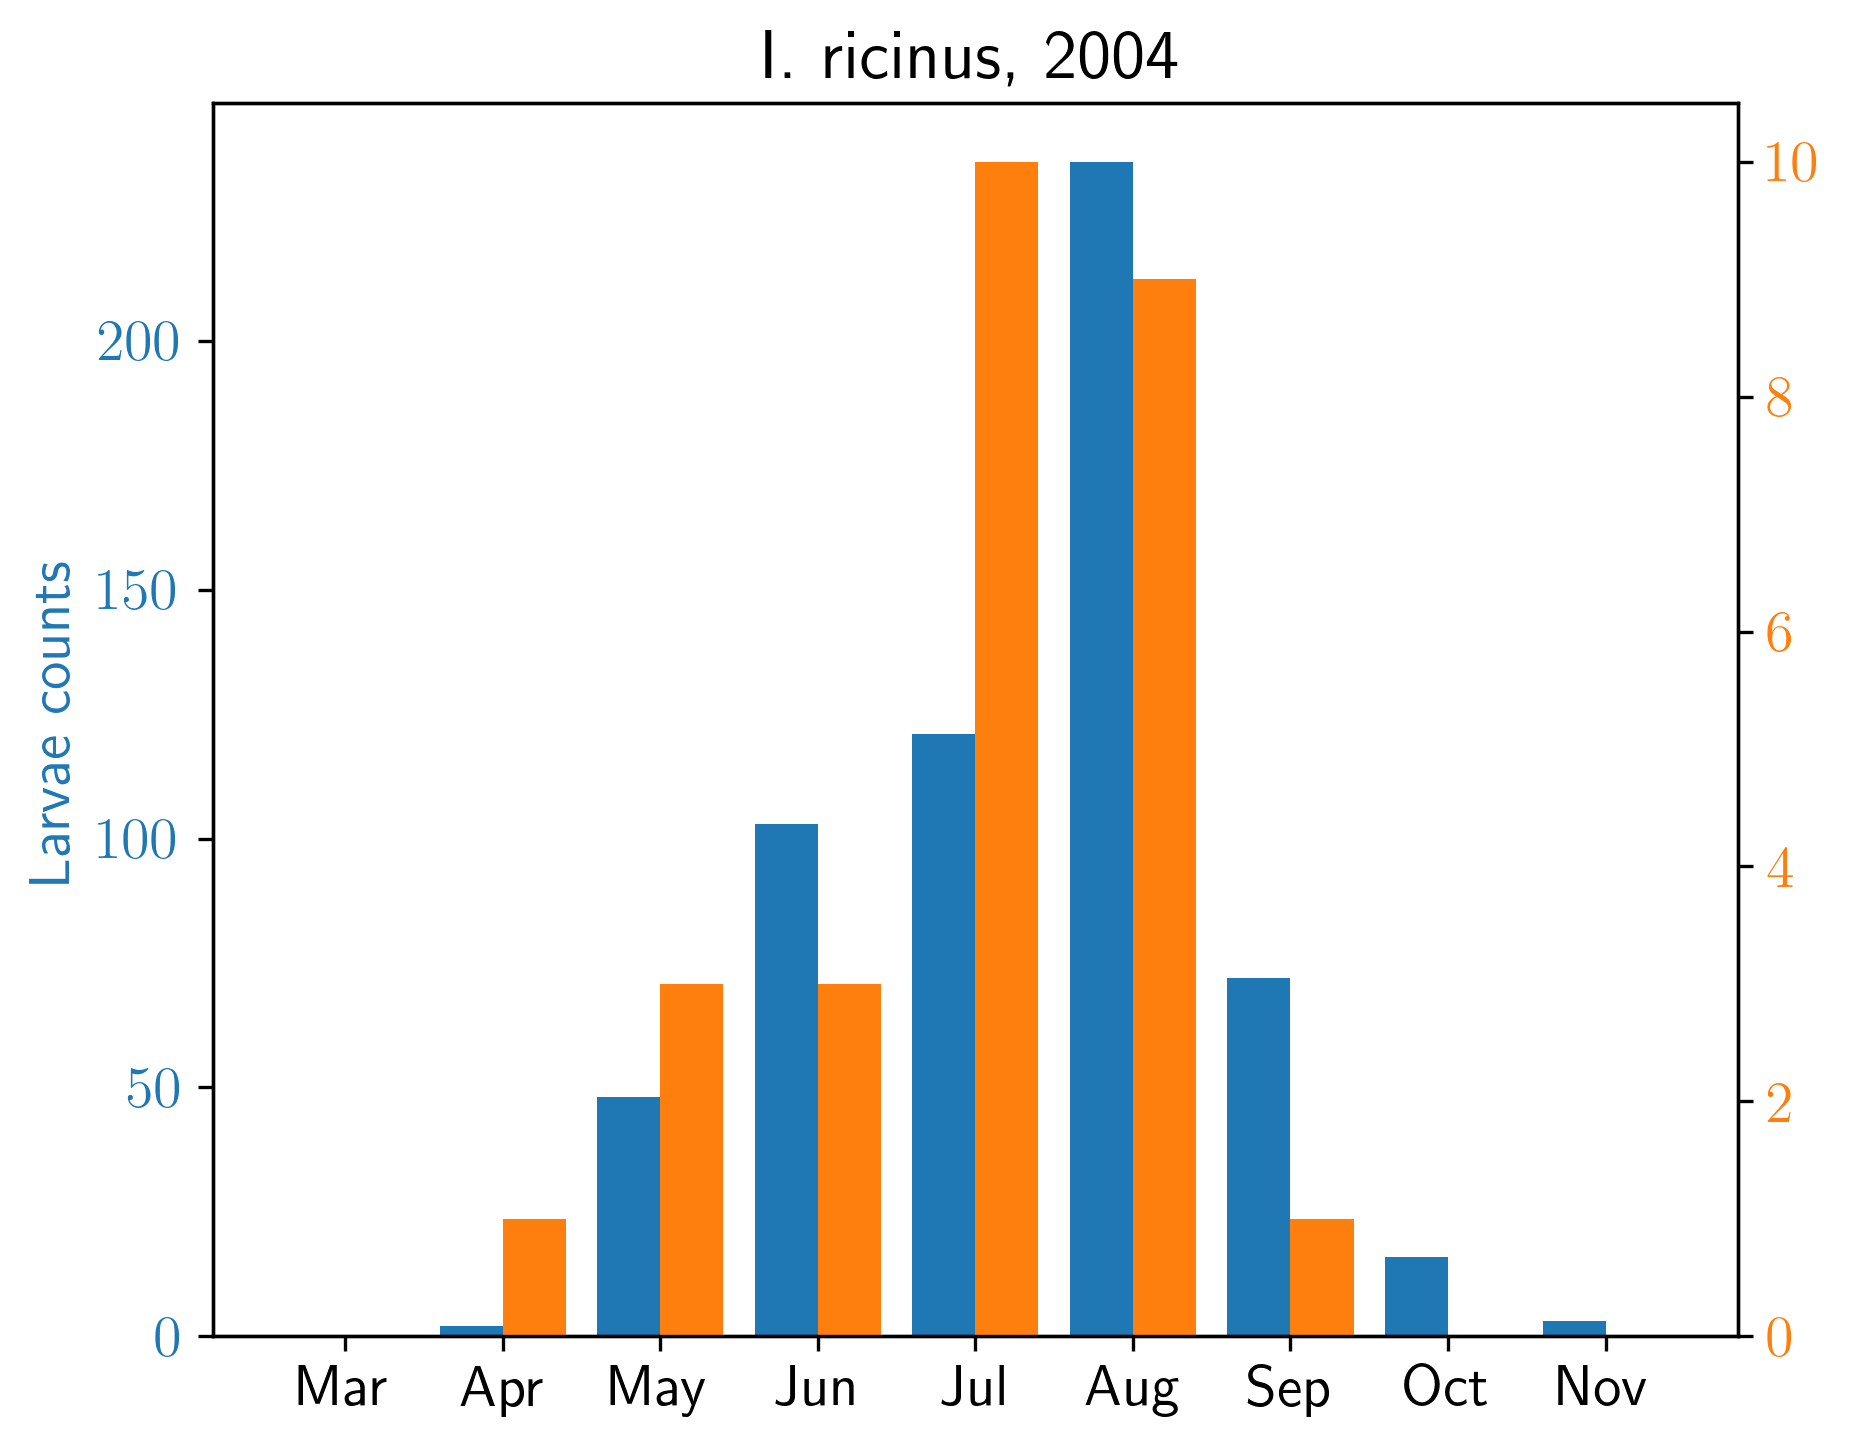
\includegraphics[width=.495\linewidth,valign=m]{I. ricinus, 2004} & 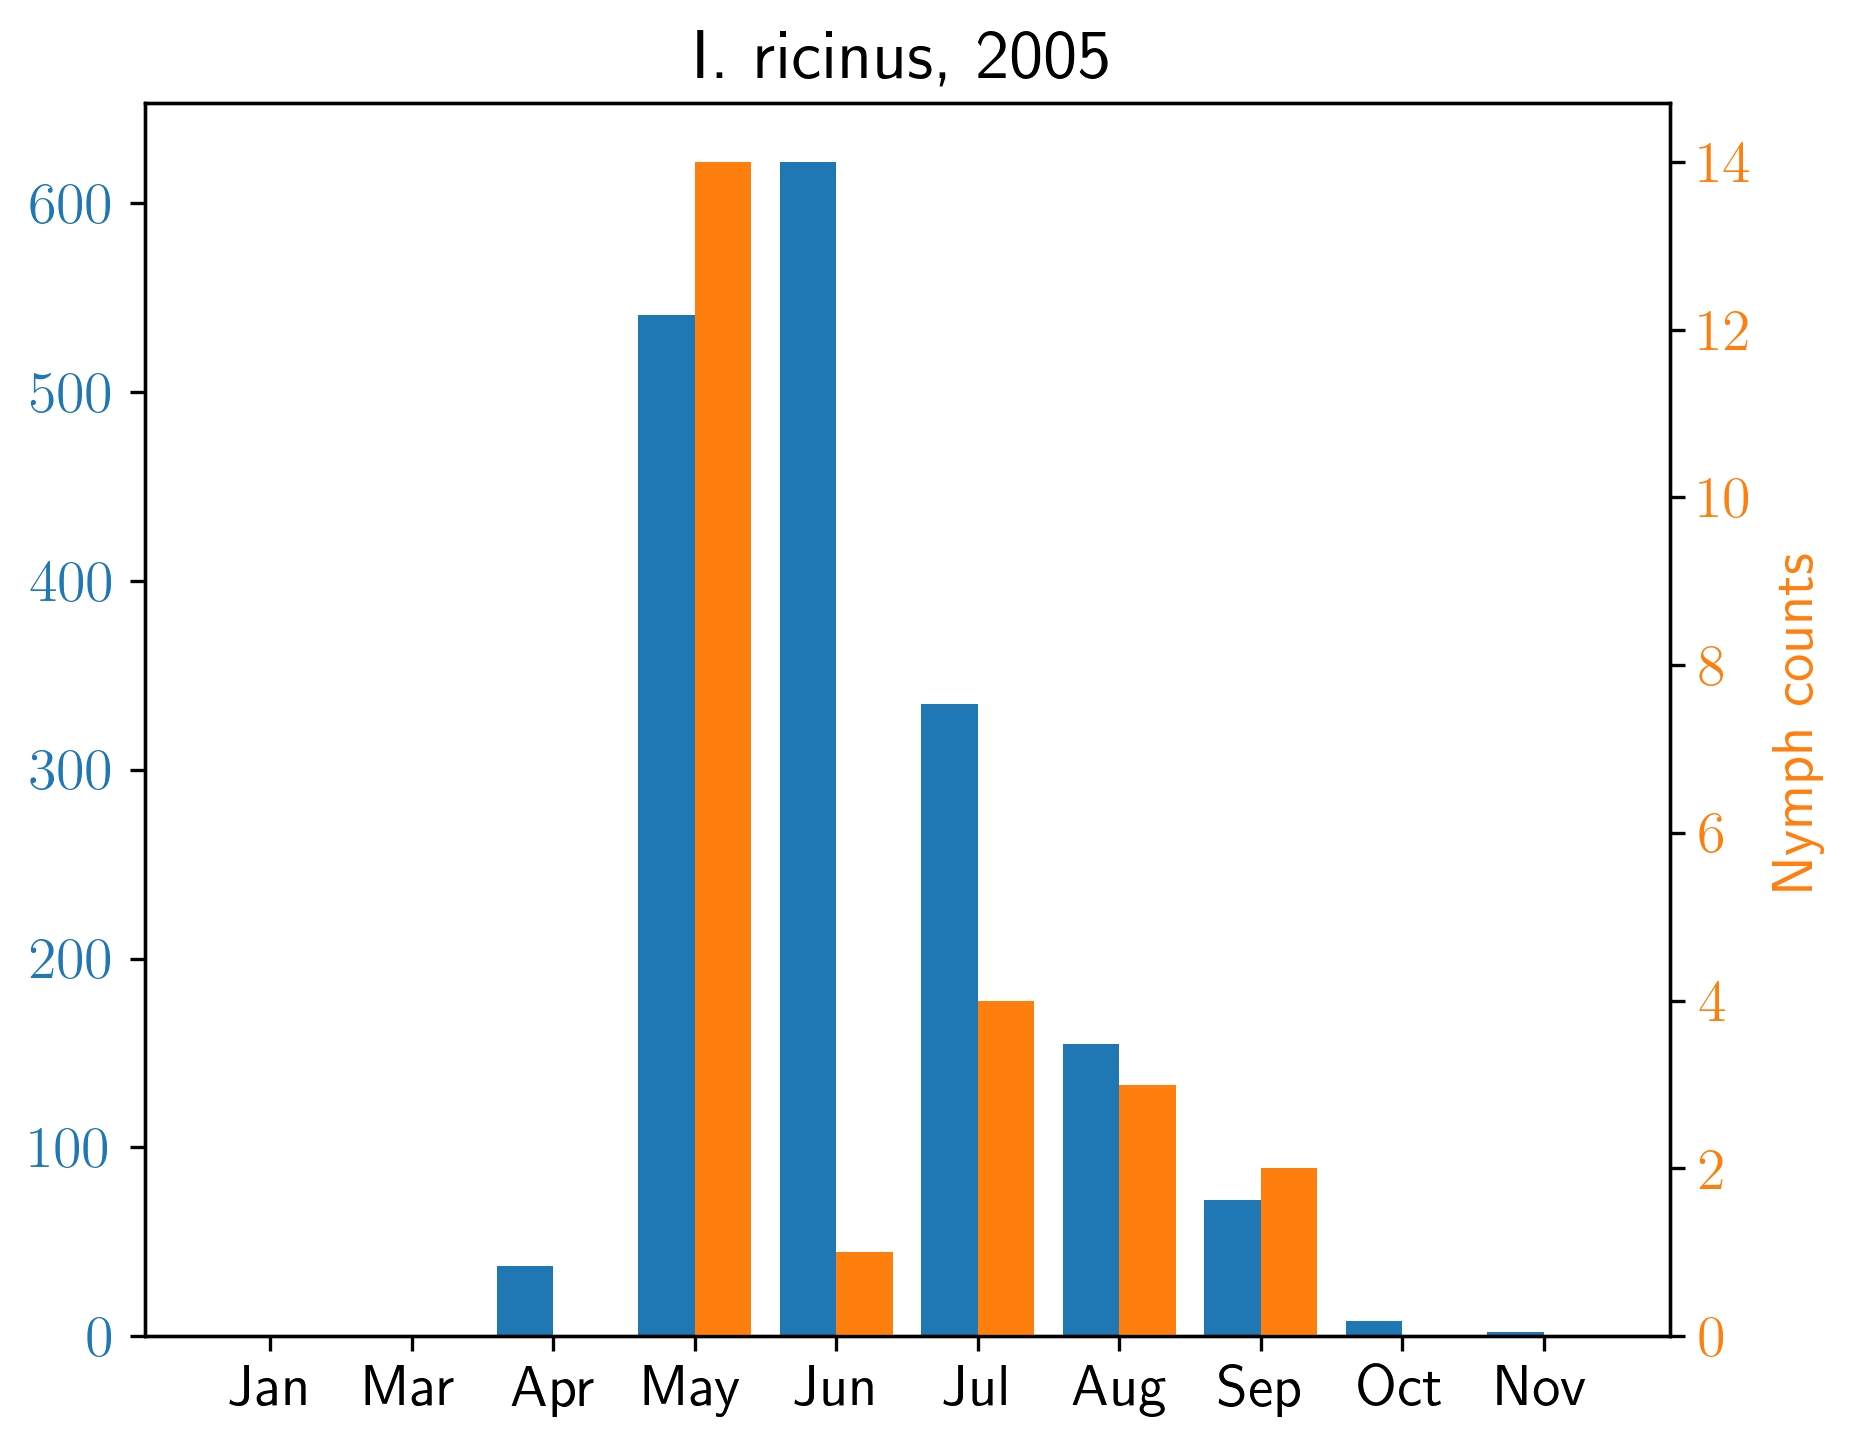
\includegraphics[width=.5\linewidth,valign=m]{I. ricinus, 2005} \\
		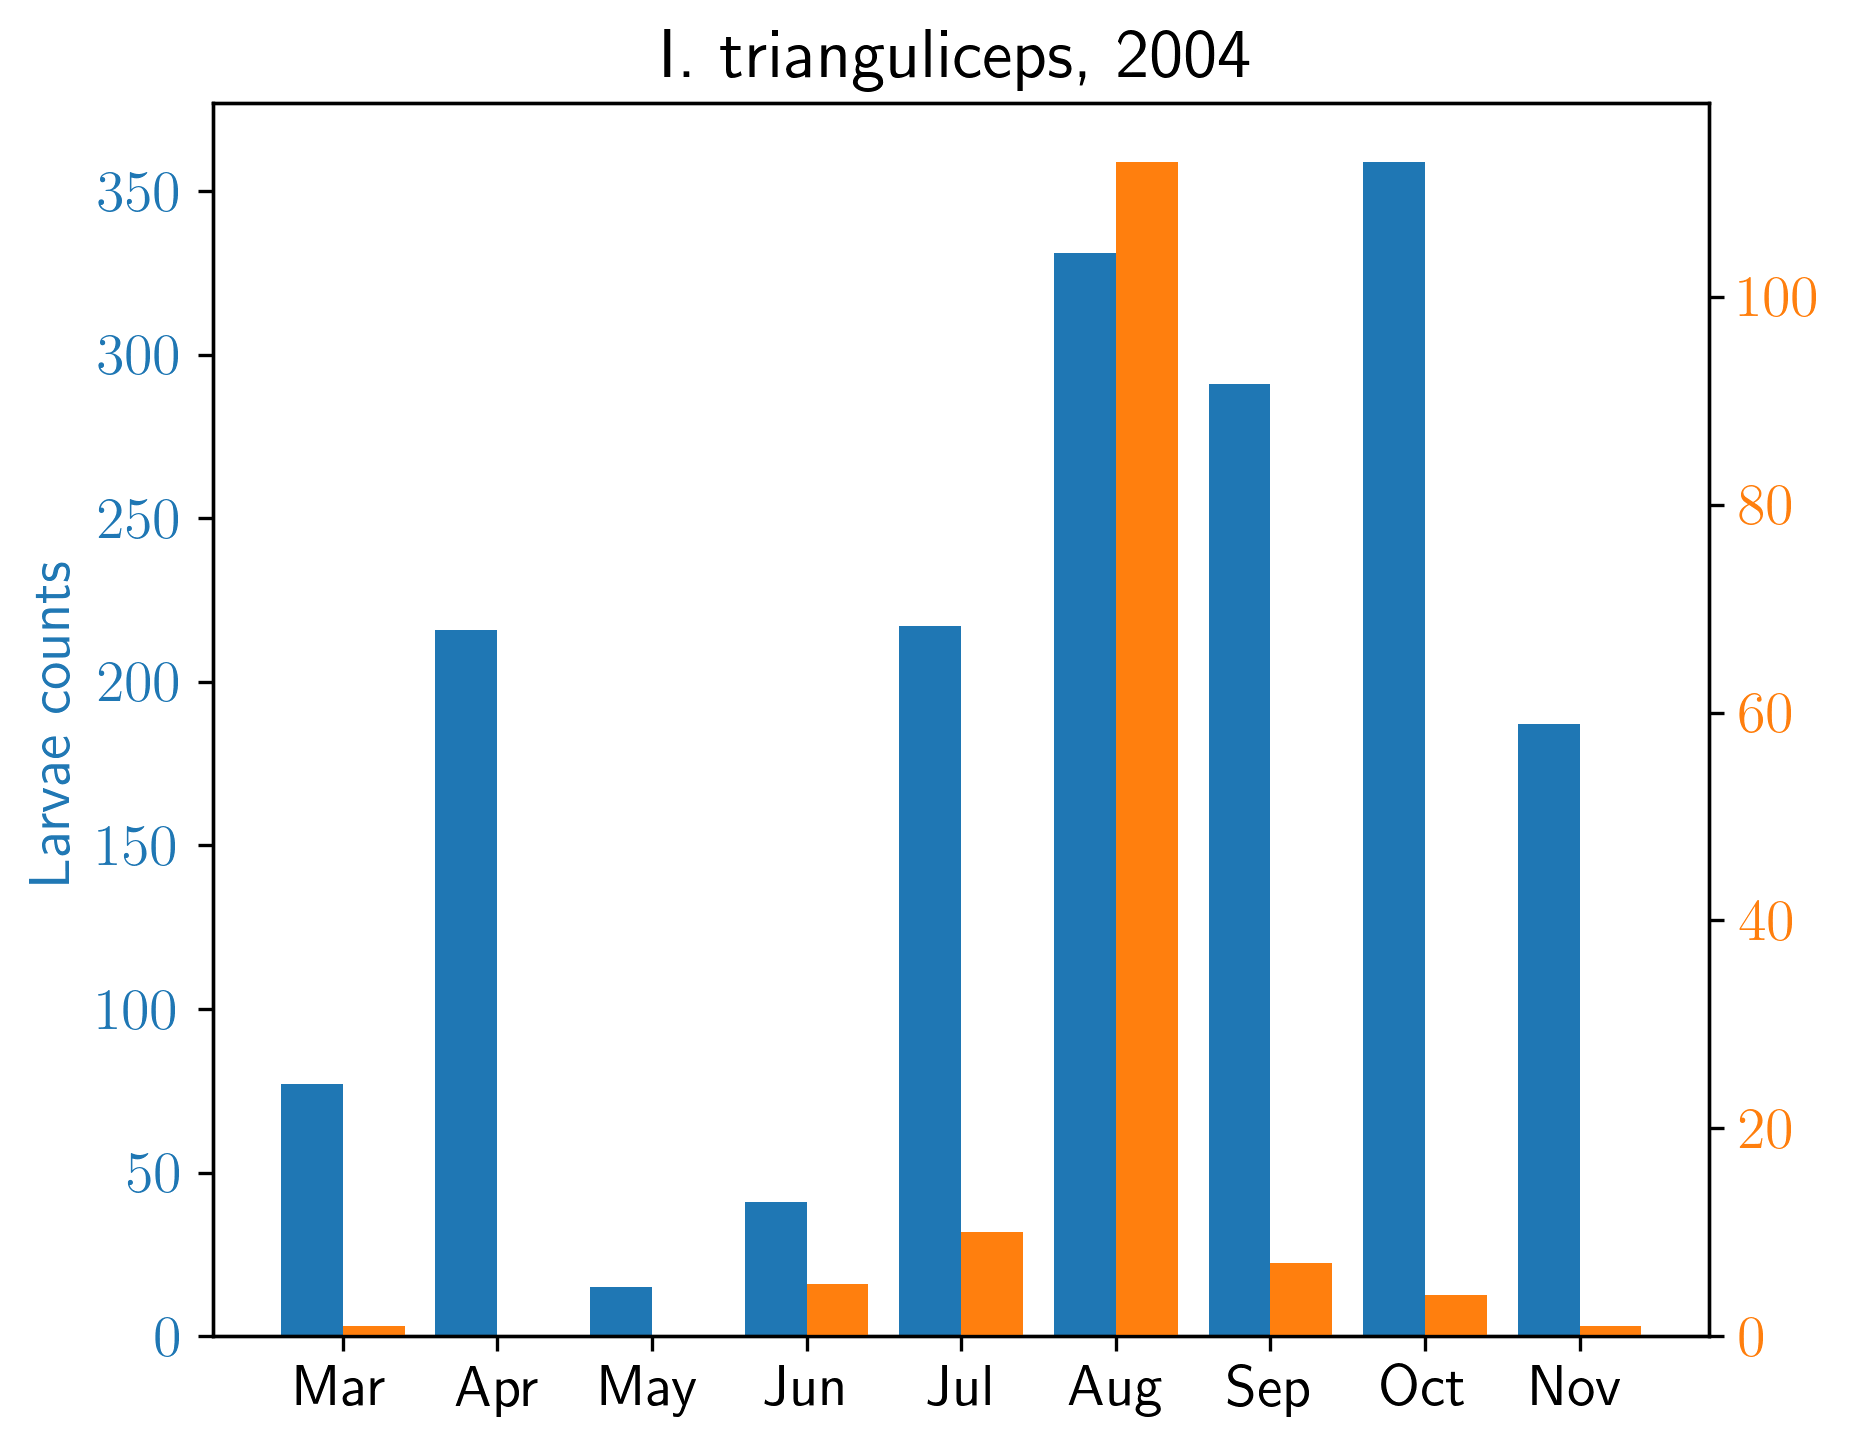
\includegraphics[width=.495\linewidth,valign=m]{I. trianguliceps, 2004} & 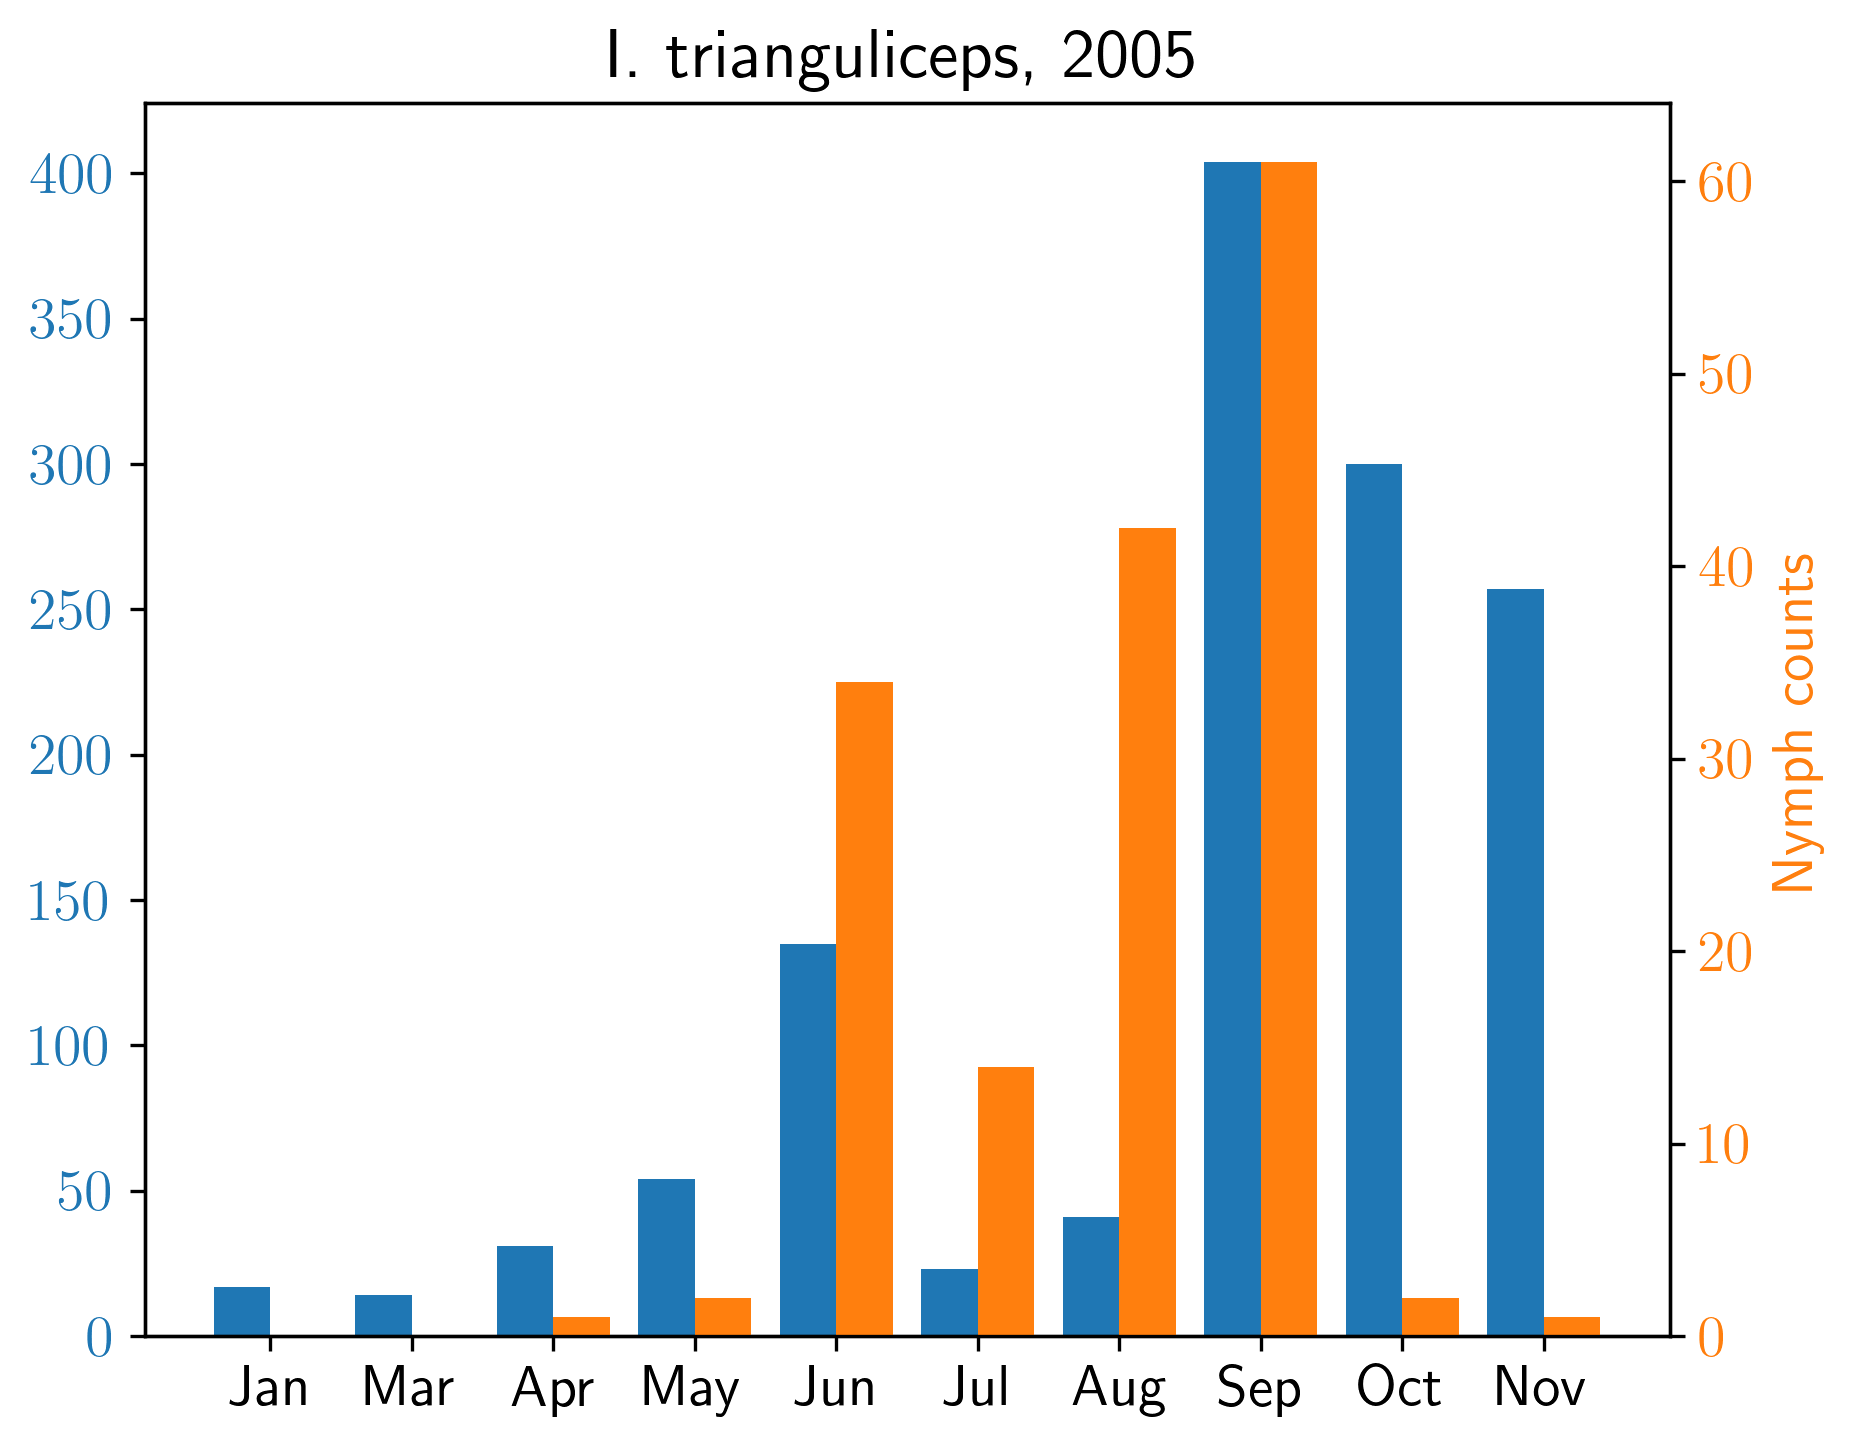
\includegraphics[width=.5\linewidth,valign=m]{I. trianguliceps, 2005} \\
	\end{tabular}
	\caption{ Seasonal nymphal and larval activity for \textit{I. trianguliceps} and \textit{I. ricinus} for 2004 and 2005. The data here shows the combined frequency of tick counts found on field vole and common shrew individuals.}
	\label{fig:kielder_seasonal}
	\end{mdframed}
\end{figure}

Overall counts of larval and nymphal burdens for both species of tick, and for the common shrew and field vole host species, are presented in Table \ref{tab:counts_kielder_overall}.

\begin{table}[]
	\begin{mdframed}[backgroundcolor=grey250,rightline=false,leftline=false,topline=false]
	\centering
	\begin{tabular}{|llrrrr|}
		\hline
		\multicolumn{6}{|c|}{\textbf{\begin{tabular}[c]{@{}c@{}}Co-aggregation data (count data) \\ Kielder Forest\end{tabular}}}                                                                               \\ \hline
		\multicolumn{2}{|l|}{\multirow{2}{*}{}}                                         & \multicolumn{2}{c|}{\textit{I. ricinus}}                  & \multicolumn{2}{c|}{\textit{I. trianguliceps}}            \\ \cline{3-6} 
		\multicolumn{2}{|l|}{}                                                          & \multicolumn{1}{l|}{Larvae} & \multicolumn{1}{l|}{Nymphs} & \multicolumn{1}{l|}{Larvae} & \multicolumn{1}{l|}{Nymphs} \\ \hline
		\multicolumn{1}{|l|}{\multirow{2}{*}{2004}} & \multicolumn{1}{l|}{Common shrew} & \multicolumn{1}{r|}{451}    & \multicolumn{1}{r|}{14}     & \multicolumn{1}{r|}{1302}   & 137                         \\ \cline{2-6} 
		\multicolumn{1}{|l|}{}                      & \multicolumn{1}{l|}{Field vole}   & \multicolumn{1}{r|}{150}    & \multicolumn{1}{r|}{13}     & \multicolumn{1}{r|}{432}    & 4                           \\ \hline
		\multicolumn{1}{|l|}{\multirow{2}{*}{2005}} & \multicolumn{1}{l|}{Common shrew} & \multicolumn{1}{r|}{314}    & \multicolumn{1}{r|}{0}      & \multicolumn{1}{r|}{512}    & 79                          \\ \cline{2-6} 
		\multicolumn{1}{|l|}{}                      & \multicolumn{1}{l|}{Field vole}   & \multicolumn{1}{r|}{1458}   & \multicolumn{1}{r|}{24}     & \multicolumn{1}{r|}{764}    & 78                          \\ \hline
	\end{tabular}
	\caption{Overall counts of nymphs and larvae, with several vertebrate host species removed due to low counts of ticks.}
	\label{tab:counts_kielder_overall}
	\end{mdframed}
\end{table}

This project makes the assumption that co-feeding is the only viable route of transmission, and that co-feeding transmission is passed from infectious nymph to larvae that are in close proximity. Furthermore, if we assume \textit{I. ricinus} and \textit{I. trianguliceps} carry pathogens for which the other tick species are not susceptible, then we can refine the data to include only the larvae that co-aggregate with nymphs of the same species, as in Table \ref{tab:counts_kielder_with_same_species_nymphs}. This means that larvae found on vertebrates without a nymphal burden of the same species were excluded.

%\begin{table}[h!]
%	\centering
%	\begin{tabular}{|llrrrr|}
%		\hline
%		\multicolumn{6}{|c|}{\textbf{\begin{tabular}[c]{@{}c@{}}Co-aggregation data (count data) \\ Kielder Forest\end{tabular}}}                                                                               \\ \hline
%		\multicolumn{2}{|l|}{\multirow{2}{*}{}}                                         & \multicolumn{2}{c|}{\textit{I. ricinus}}                  & \multicolumn{2}{c|}{\textit{I. trianguliceps}}            \\ \cline{3-6} 
%		\multicolumn{2}{|l|}{}                                                          & \multicolumn{1}{l|}{Larvae} & \multicolumn{1}{l|}{Nymphs} & \multicolumn{1}{l|}{Larvae} & \multicolumn{1}{l|}{Nymphs} \\ \hline
%		\multicolumn{1}{|l|}{\multirow{2}{*}{2004}} & \multicolumn{1}{l|}{Common shrew} & \multicolumn{1}{r|}{180}    & \multicolumn{1}{r|}{14}     & \multicolumn{1}{r|}{377}    & 137                         \\ \cline{2-6} 
%		\multicolumn{1}{|l|}{}                      & \multicolumn{1}{l|}{Field vole}   & \multicolumn{1}{r|}{8}     & \multicolumn{1}{r|}{13}     & \multicolumn{1}{r|}{1}     & 4                          \\ \hline
%		\multicolumn{1}{|l|}{\multirow{2}{*}{2005}} & \multicolumn{1}{l|}{Common shrew} & \multicolumn{1}{r|}{80}     & \multicolumn{1}{r|}{0}     & \multicolumn{1}{r|}{179}    & 79                          \\ \cline{2-6} 
%		\multicolumn{1}{|l|}{}                      & \multicolumn{1}{l|}{Field vole}   & \multicolumn{1}{r|}{242}    & \multicolumn{1}{r|}{24}     & \multicolumn{1}{r|}{14}     & 78                          \\ \hline
%	\end{tabular}
%	\caption{Counts of nymphs and larvae on vertebrates where one or more nymphs were found.}
%	\label{tab:counts_kielder_with_nymphs}
%\end{table}


\begin{table}[]
	\begin{mdframed}[backgroundcolor=grey250,rightline=false,leftline=false,topline=false]
	\centering
	\begin{tabular}{|llrrrr|}
		\hline
		\multicolumn{6}{|c|}{\textbf{\begin{tabular}[c]{@{}c@{}}Co-aggregation data (count data) \\ Kielder Forest\end{tabular}}}                                                                               \\ \hline
		\multicolumn{2}{|l|}{\multirow{2}{*}{}}                                         & \multicolumn{2}{c|}{\textit{I. ricinus}}                  & \multicolumn{2}{c|}{\textit{I. trianguliceps}}            \\ \cline{3-6} 
		\multicolumn{2}{|l|}{}                                                          & \multicolumn{1}{l|}{Larvae} & \multicolumn{1}{l|}{Nymphs} & \multicolumn{1}{l|}{Larvae} & \multicolumn{1}{l|}{Nymphs} \\ \hline
		\multicolumn{1}{|l|}{\multirow{2}{*}{2004}} & \multicolumn{1}{l|}{Common shrew} & \multicolumn{1}{r|}{48}     & \multicolumn{1}{r|}{14}     & \multicolumn{1}{r|}{369}    & 137                         \\ \cline{2-6} 
		\multicolumn{1}{|l|}{}                      & \multicolumn{1}{l|}{Field vole}   & \multicolumn{1}{r|}{7}      & \multicolumn{1}{r|}{13}     & \multicolumn{1}{r|}{1}      & 4                           \\ \hline
		\multicolumn{1}{|l|}{\multirow{2}{*}{2005}} & \multicolumn{1}{l|}{Common shrew} & \multicolumn{1}{r|}{0}      & \multicolumn{1}{r|}{0}      & \multicolumn{1}{r|}{179}    & 79                          \\ \cline{2-6} 
		\multicolumn{1}{|l|}{}                      & \multicolumn{1}{l|}{Field vole}   & \multicolumn{1}{r|}{190}    & \multicolumn{1}{r|}{24}     & \multicolumn{1}{r|}{9}      & 78                          \\ \hline
	\end{tabular}
	\caption{Counts of nymphs and counts of larvae that co-feed with nymphs of the same species.}
	\label{tab:counts_kielder_with_same_species_nymphs}
	\end{mdframed}
\end{table}

Based on low tick burden counts, we exclude several combinations but will investigate these combinations using the Kielder Forest data:
\begin{itemize}
    \item 2004: \textit{I. ricinus} found on common shrews.
    \item 2004: \textit{I. trianguliceps} found on common shrews.
    \item 2005: \textit{I. trianguliceps} found on common shrews.
    \item 2005: \textit{I. ricinus} found on field voles.
    \item 2005: \textit{I. trianguliceps} found on field voles.
\end{itemize}

There are several sensible reasons to separate these data into these 5 separate categories, rather than analysing all data together:

\begin{itemize}
    \item \textit{I. ricinus} is non-nidicolous while \textit{I. trianguliceps} is nidicolous, indicating different behaviour \cite{}.
    \item The pathogens transmitted by each tick species are frequently not the same pathogens \cite{}.
    \item An adult common shrew is larger than the adult field vole \cite{}, which implies the probability of nymphs and larvae co-feeding on a field vole, but in close enough proximity for co-feeding transmission to occur, is greater than for ticks that co-feed on common shrews. 
    \item The two species of vertebrate host might have different rates of attracting ticks.
    \item Yearly seasonal variation shown in Figure \ref{fig:kielder_seasonal} suggests that these ticks have peak activities at different times of the year.
\end{itemize}

Central to this project is the co-incident co-aggregation of juvenile ticks on vertebrate hosts. To check the data reflected this, we used the Spearman Correlation Coefficient to test the existence of a monotonic relationship; generally, the vertebrate hosts that have more nymphs should also have more larvae. 
We used the SciPy package in Python to perform the test. We found weak evidence of correlation for some host and tick combinations. The results presented in Table \ref{tab:spearman_kielder}.

\begin{table}[ht]
	\begin{mdframed}[backgroundcolor=grey250,rightline=false,leftline=false,topline=false]
	\centering
	\begin{tabular}{|lrrrr|}
		\hline
		\multicolumn{5}{|c|}{\textbf{\begin{tabular}[c]{@{}c@{}}Spearman (ranked) Correlation Analysis \\ Kielder Forest\end{tabular}}}         \\ \hline
		\multicolumn{1}{|l|}{\multirow{2}{*}{}}                                                      & \multicolumn{2}{c|}{\textit{I. ricinus}}                             & \multicolumn{2}{c|}{\textit{I. trianguliceps}}                        \\ \cline{2-5} 
		\multicolumn{1}{|l|}{}                                                                       & \multicolumn{1}{l|}{statistic}    & \multicolumn{1}{l|}{p-value} & \multicolumn{1}{l|}{statistic}     & \multicolumn{1}{l|}{p-value} \\ \hline
		\multicolumn{1}{|l|}{Common shrew}                                                           & \multicolumn{1}{r|}{0.13401} & \multicolumn{1}{r|}{$\sim$0} & \multicolumn{1}{r|}{0.24473}  & $\sim$0                      \\ \hline
		\multicolumn{1}{|l|}{Field vole}                                                             & \multicolumn{1}{r|}{0.22757} & \multicolumn{1}{r|}{$\sim$0} & \multicolumn{1}{r|}{-0.03027} & 0.10164                      \\ \hline
		\multicolumn{1}{|l|}{\begin{tabular}[c]{@{}l@{}}Common shrew \\ and field vole\end{tabular}} & \multicolumn{1}{r|}{0.19450} & \multicolumn{1}{r|}{$\sim$0} & \multicolumn{1}{r|}{0.12317}  & $\sim$0                      \\ \hline
	\end{tabular}
	\caption{The ranked correlations between nymphs and larvae, obtained by analysing the Kielder Forest data provided by Bown et al. }
	\label{tab:spearman_kielder}
	\end{mdframed}
\end{table}

Assuming confidence of $ 0.95 $, then the pvalue $ > 0.05 $ of \textit{I.trianguliceps} on field voles means we cannot reject the null hypothesis that there does not exist a monotonic relationship between the counts of larvae and nymphs for that combination of tick and host species. This pair of tick and vertebrate host species also has the lowest overall number of larvae, indicating low levels of co-aggregation. It is interesting that later in this project, we show co-feeding transmission between \textit{I. trianguliceps} that co-feed on \textit{Field Voles} will not allow for a pathogen's survival.

\subsection{Tick burden heterogeneity} 

Some vertebrate hosts attract many more ticks than others, and measuring that heterogeneity has been addressed or estimated in many studies \cite{}. Of particular interest is research from Perkins et al in 2003 \cite{Perkins_2003}, which quantified inequality of hosts' co-feeding transmission potentials by plotting Lorenz curves, and then calculating a Gini coefficient to describe the overall inequality. This project will also use Lorenz curves and Gini coefficients to quantify the heterogeneity of tick burdens for particular populations of vertebrate hosts. While this thesis takes inspiration from the work of Perkins et al \cite{Perkins_2003}, we use a different calculation inspired by the work of Johnstone-Robertson et al \cite{JohnstoneRobertson2020}.

A limitation of using the formula presented by Perkins et al is that burdens of ticks in different life stages are grouped together in the term $ v_i^2 $. However, this project makes the simplifying assumption that co-feeding transmission is from infected nymph to nearby larvae only. Given that simplifying assumption, the Perkins calculation is unsuitable since it will not reflect that co-feeding transmission will not occur when either the larval or nymphal burdens for a particular vertebrate host are $ 0 $. Therefore, this project seeks another method to measure the inequalities in transmission potentials that vertebrate hosts have, due to heterogeneity in co-aggregation observed on those hosts. We use a modified version of the Johnstone-Robertson formula \eqref{JohnstoneRobertsonR0Estimate} since it addresses the above-mentioned complaint.

In the Johnstone-Robertson paper, an important nuance is that $ k_{in} $ and $ k_{out} $ are respectively the nymphal and larval burdens of a host during its lifetime; to apply the calculation of $ R_0 $ to co-feeding transmission, a term $ \nu_{ln} $ is needed to consider temporal and spatial requirements. But, if we use tick burden data collected in field surveys (as with the Kielder Forest data) then we can guarantee that the temporal requirement for co-feeding transmission to occur - that there must be co-incident co-aggregation - is satisfied.

So, let:

\begin{description}[leftmargin=1cm, style=nextline]
	\item[$ b_n $] be the nymphal burden observed on an individual vertebrate host, which is analogous to $ k_{in} $, except that $ b_n $ only applies at the time of data collection.
	\item[$ b_l $] be the larval burden observed, which is analogous to $ k_{out} $.
	\item[$ m $] be the number of vertebrate hosts.
\end{description}

The modified version of \eqref{JohnstoneRobertsonR0Estimate} is now:
 
\begin{align} 
	R_0 \propto \frac{\langle b_n b_l \rangle}{\langle b_l \rangle} &= \frac{(1/m)\sum_{a=1}^m (b_n b_l)_a}{(1/m)\sum_{a=1}^m (b_n)_a} \nonumber \\ 
																	&= \frac{\sum_{a=1}^m (b_n b_l )_a}{\sum_{a=1}^m (b_l)_a} \nonumber \\ 
																	&= \frac{(b_n b_l)_1}{\sum_{a=1}^m (b_l)_a} + \frac{(b_n b_l)_2}{\sum_{a=1}^m (b_l)_a} + ... + \frac{(b_n b_l)_m}{\sum_{a=1}^m (b_l)_a} \label{JohnstoneRobertsonR0Cumulative}
\end{align}

The goal is to obtain a cumulative estimate of vertebrate hosts' contributions to total transmission potentials, but without first having to find $ R_0 $, as did the example set by Perkins et al. We can order the vertebrates by the product $ b_n b_l $ in descending order, with $ a=1 $ denoting the vertebrate with the largest relative transmission potential. Then, we remove groups of vertebrates that have the most transmission potentials, following the Perkins et al example. The cumulative effect of removing subsequently larger whole-number percentages of vertebrate hosts is shown in Figures \ref{fig:lorenz_2004_iricinus_SA}, \ref{fig:lorenz_2004_itrianguliceps_SA}, \ref{fig:lorenz_2005_itrianguliceps_SA}, \ref{fig:lorenz_2005_iricinus_FV}, \ref{fig:lorenz_2005_itrianguliceps_FV}. In those figures, the cumulative totals for tick aggregation (total numbers of nymph and larvae) are plotted next to the cumulative transmission potential of calculated by using \eqref{JohnstoneRobertsonR0Cumulative}. Each curve is found by removing subsequently larger proportions of the vertebrate host populations, starting with 1\%, then 2\%, and so on. The shape of each Lorenz curve is useful as a visual aide for understanding the inequality in transmission potentials. We also use those to calculate Gini coefficients, which are reported in Table \ref{tab:kielderGINI}.

\begin{figure}[]
	\begin{mdframed}[backgroundcolor=grey250,rightline=false,leftline=false,topline=false]
	\centering
	\begin{tabular}{ll}
		\includegraphics[width=.48\linewidth,valign=m]{lorenz_aggregation_SA_2004_I.Ricinus} & \includegraphics[width=.48\linewidth,valign=m]{lorenz_JR_SA_2004_I.Ricinus} \\
	\end{tabular}
	\caption{Aggregation (left) and cumulative transmission potential (right) of \textit{common shrews} that were found with \textit{I.  ricinus} in \textit{2004} in the Kielder Forest data.}
	\label{fig:lorenz_2004_iricinus_SA}
	\end{mdframed}
\end{figure}

\begin{figure}[]
	\begin{mdframed}[backgroundcolor=grey250,rightline=false,leftline=false,topline=false]
	\centering
	\begin{tabular}{ll}
		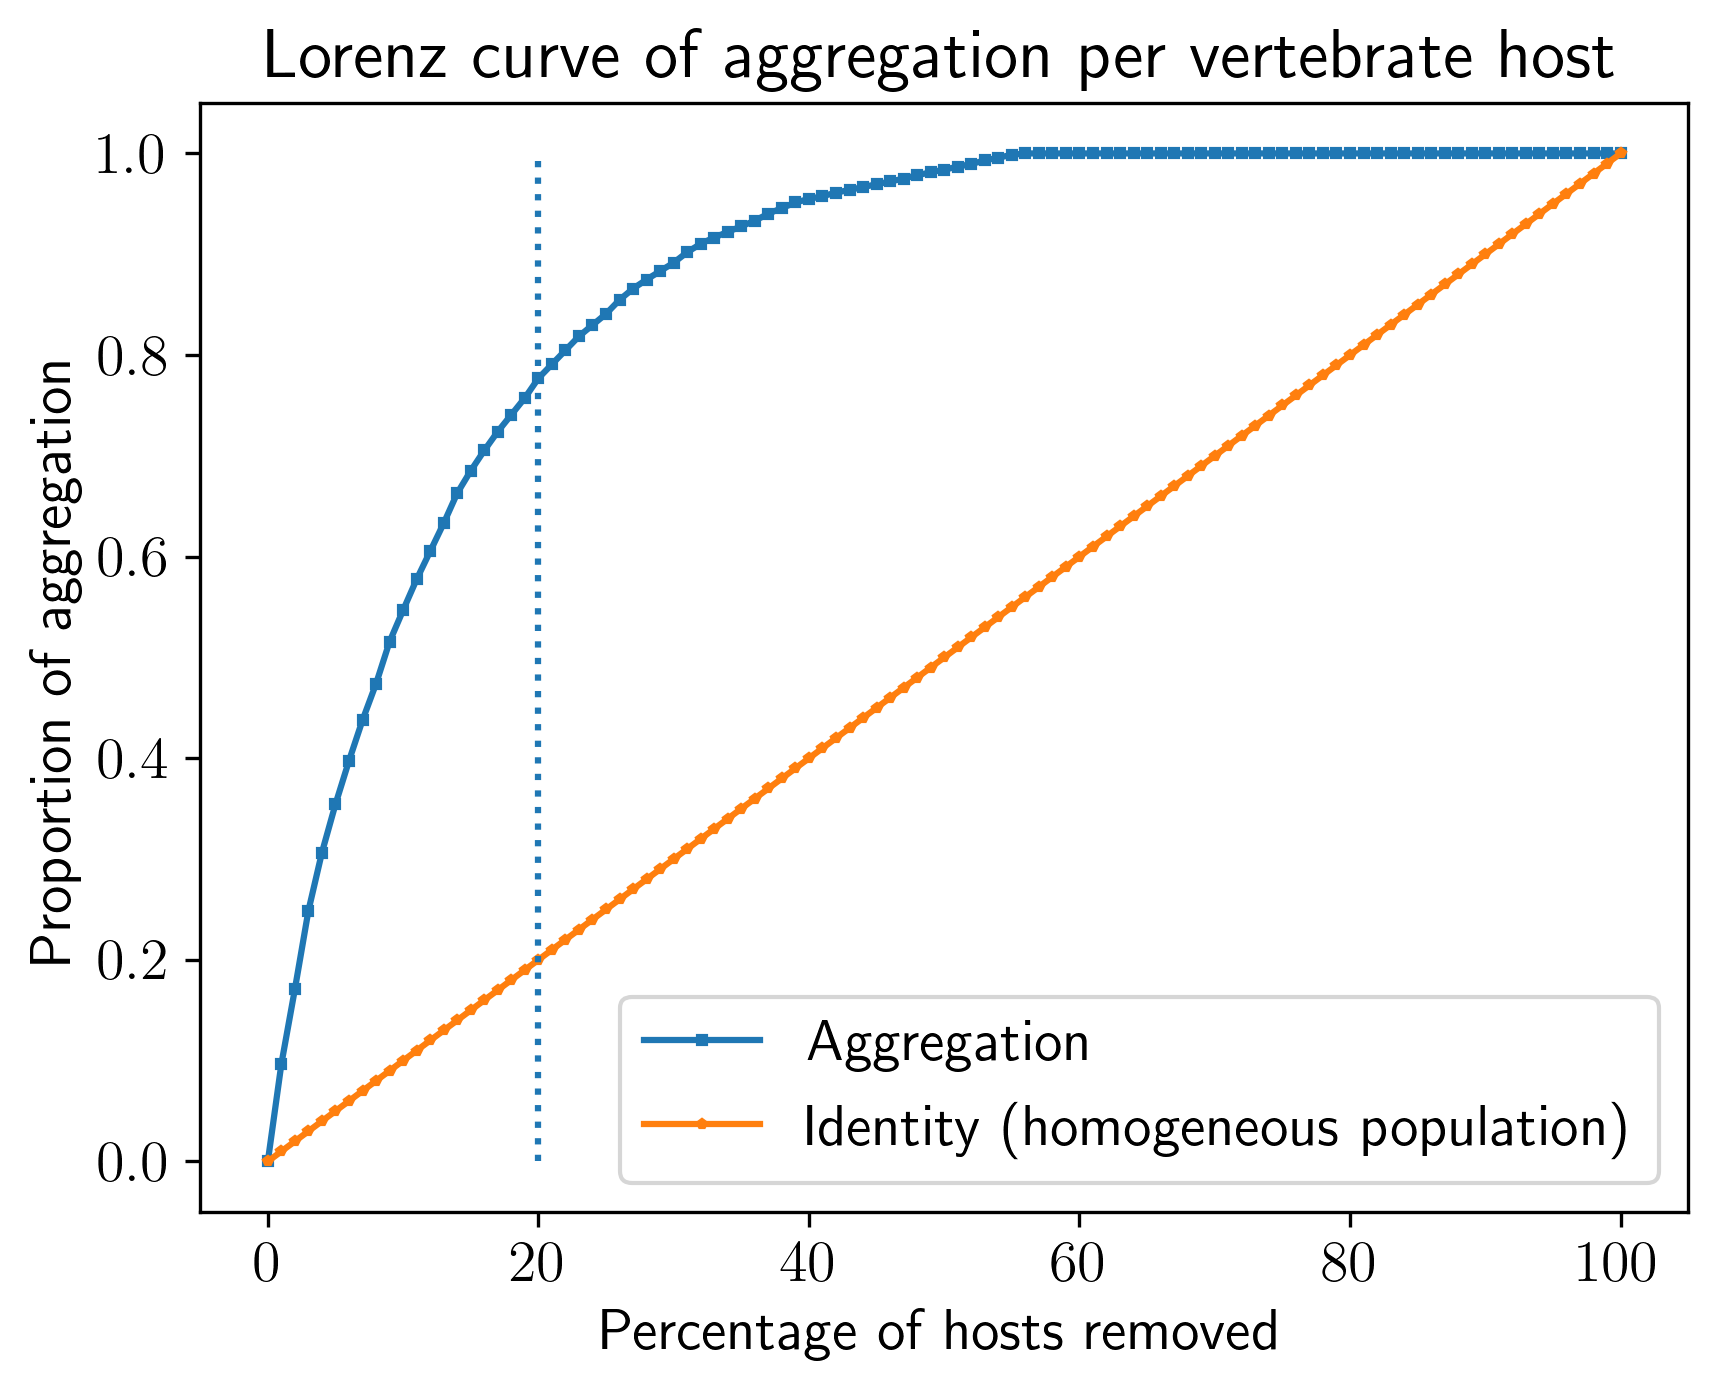
\includegraphics[width=.48\linewidth,valign=m]{lorenz_aggregation_SA_2004_I.Trianguliceps} & 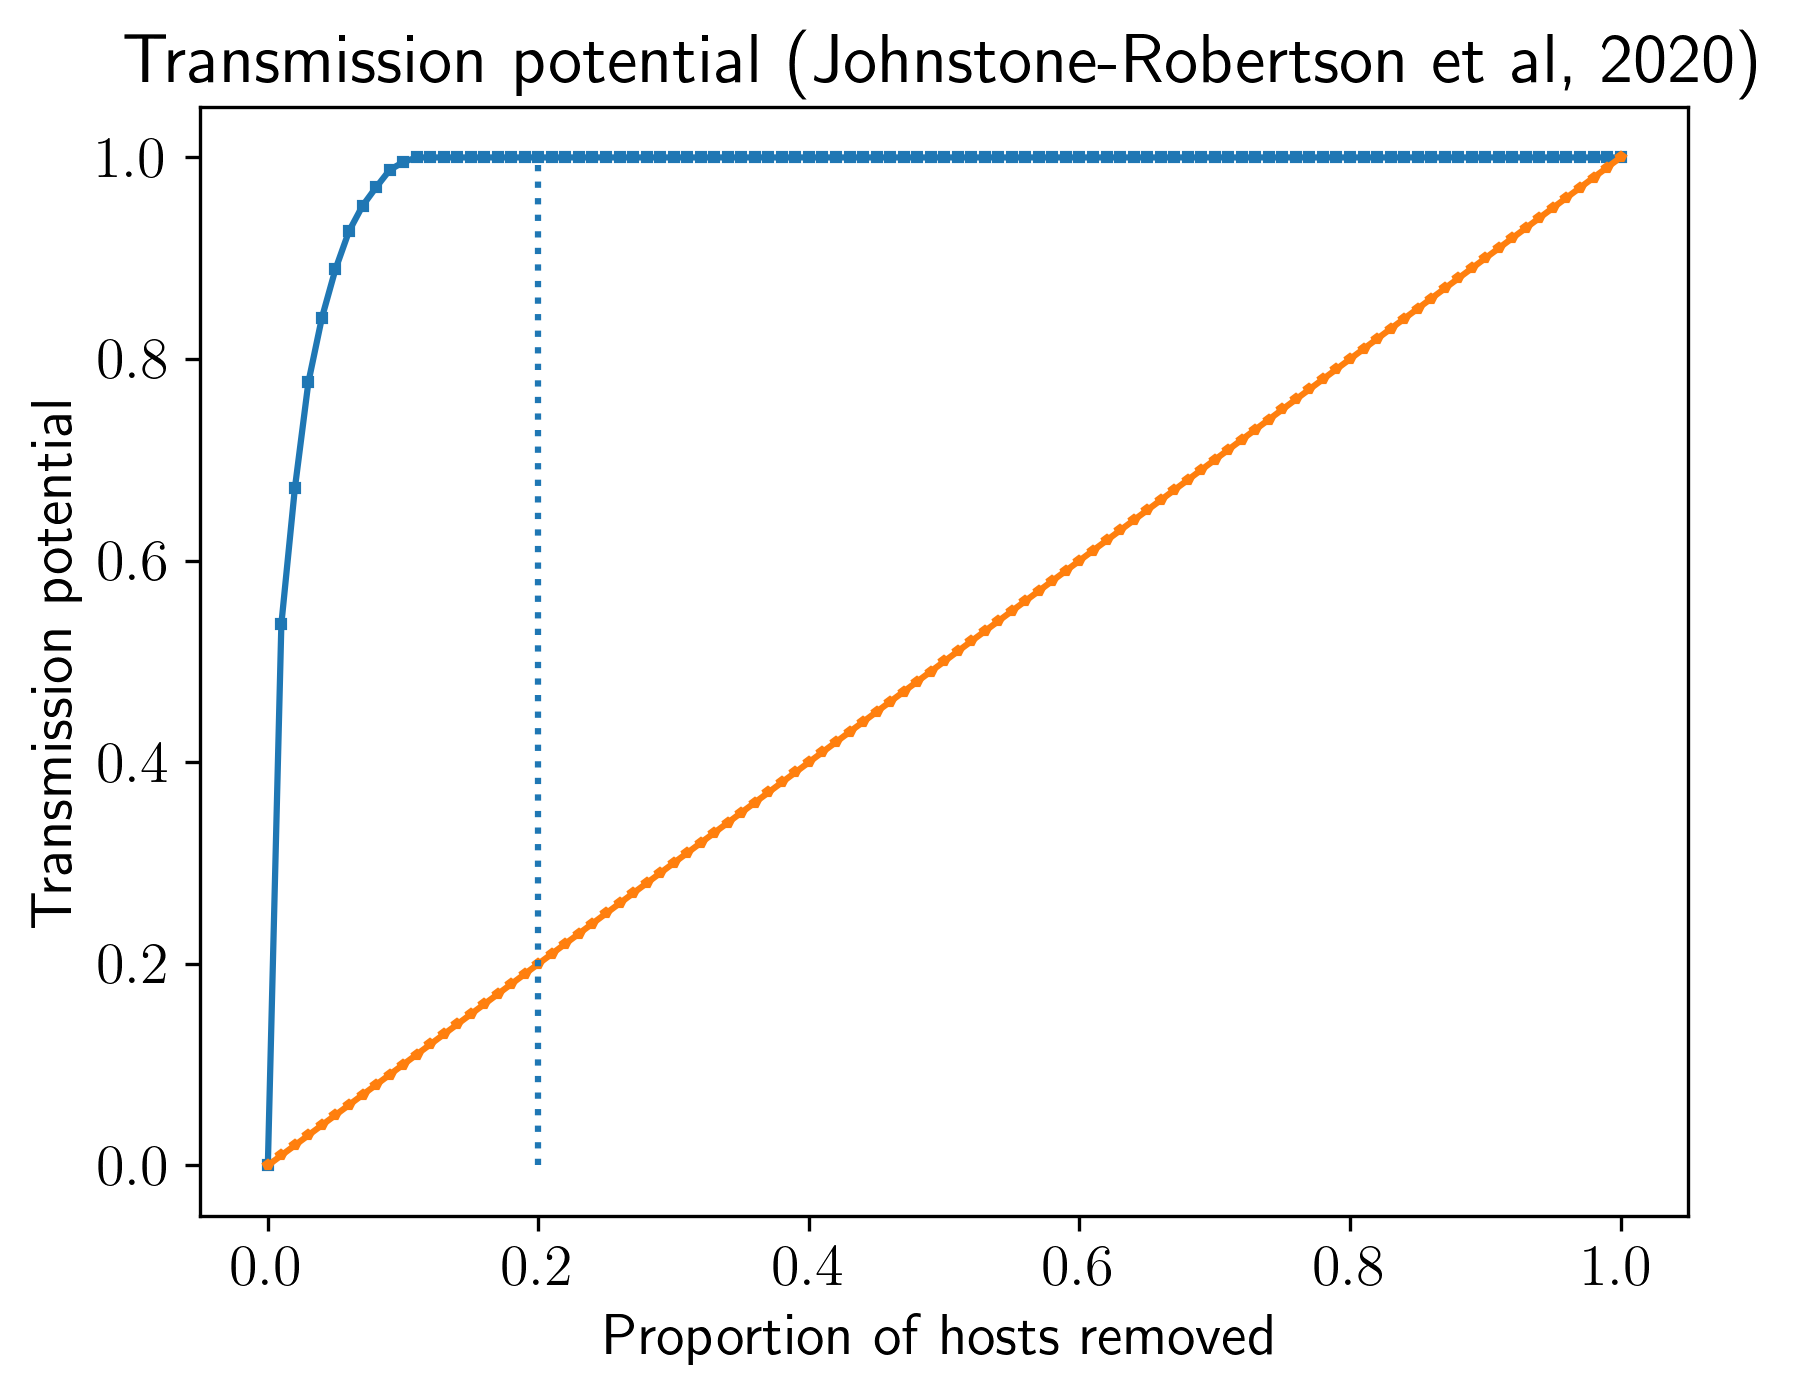
\includegraphics[width=.48\linewidth,valign=m]{lorenz_JR_SA_2004_I.Trianguliceps} \\
	\end{tabular}
	\caption{Aggregation (left) and cumulative transmission potential (right) of \textit{common shrews} that were found with \textit{I. trianguliceps} in \textit{2004} in the Kielder Forest data.}
	\label{fig:lorenz_2004_itrianguliceps_SA}
	\end{mdframed}
\end{figure}

\begin{figure}[]
	\begin{mdframed}[backgroundcolor=grey250,rightline=false,leftline=false,topline=false]
	\centering
	\begin{tabular}{ll}
		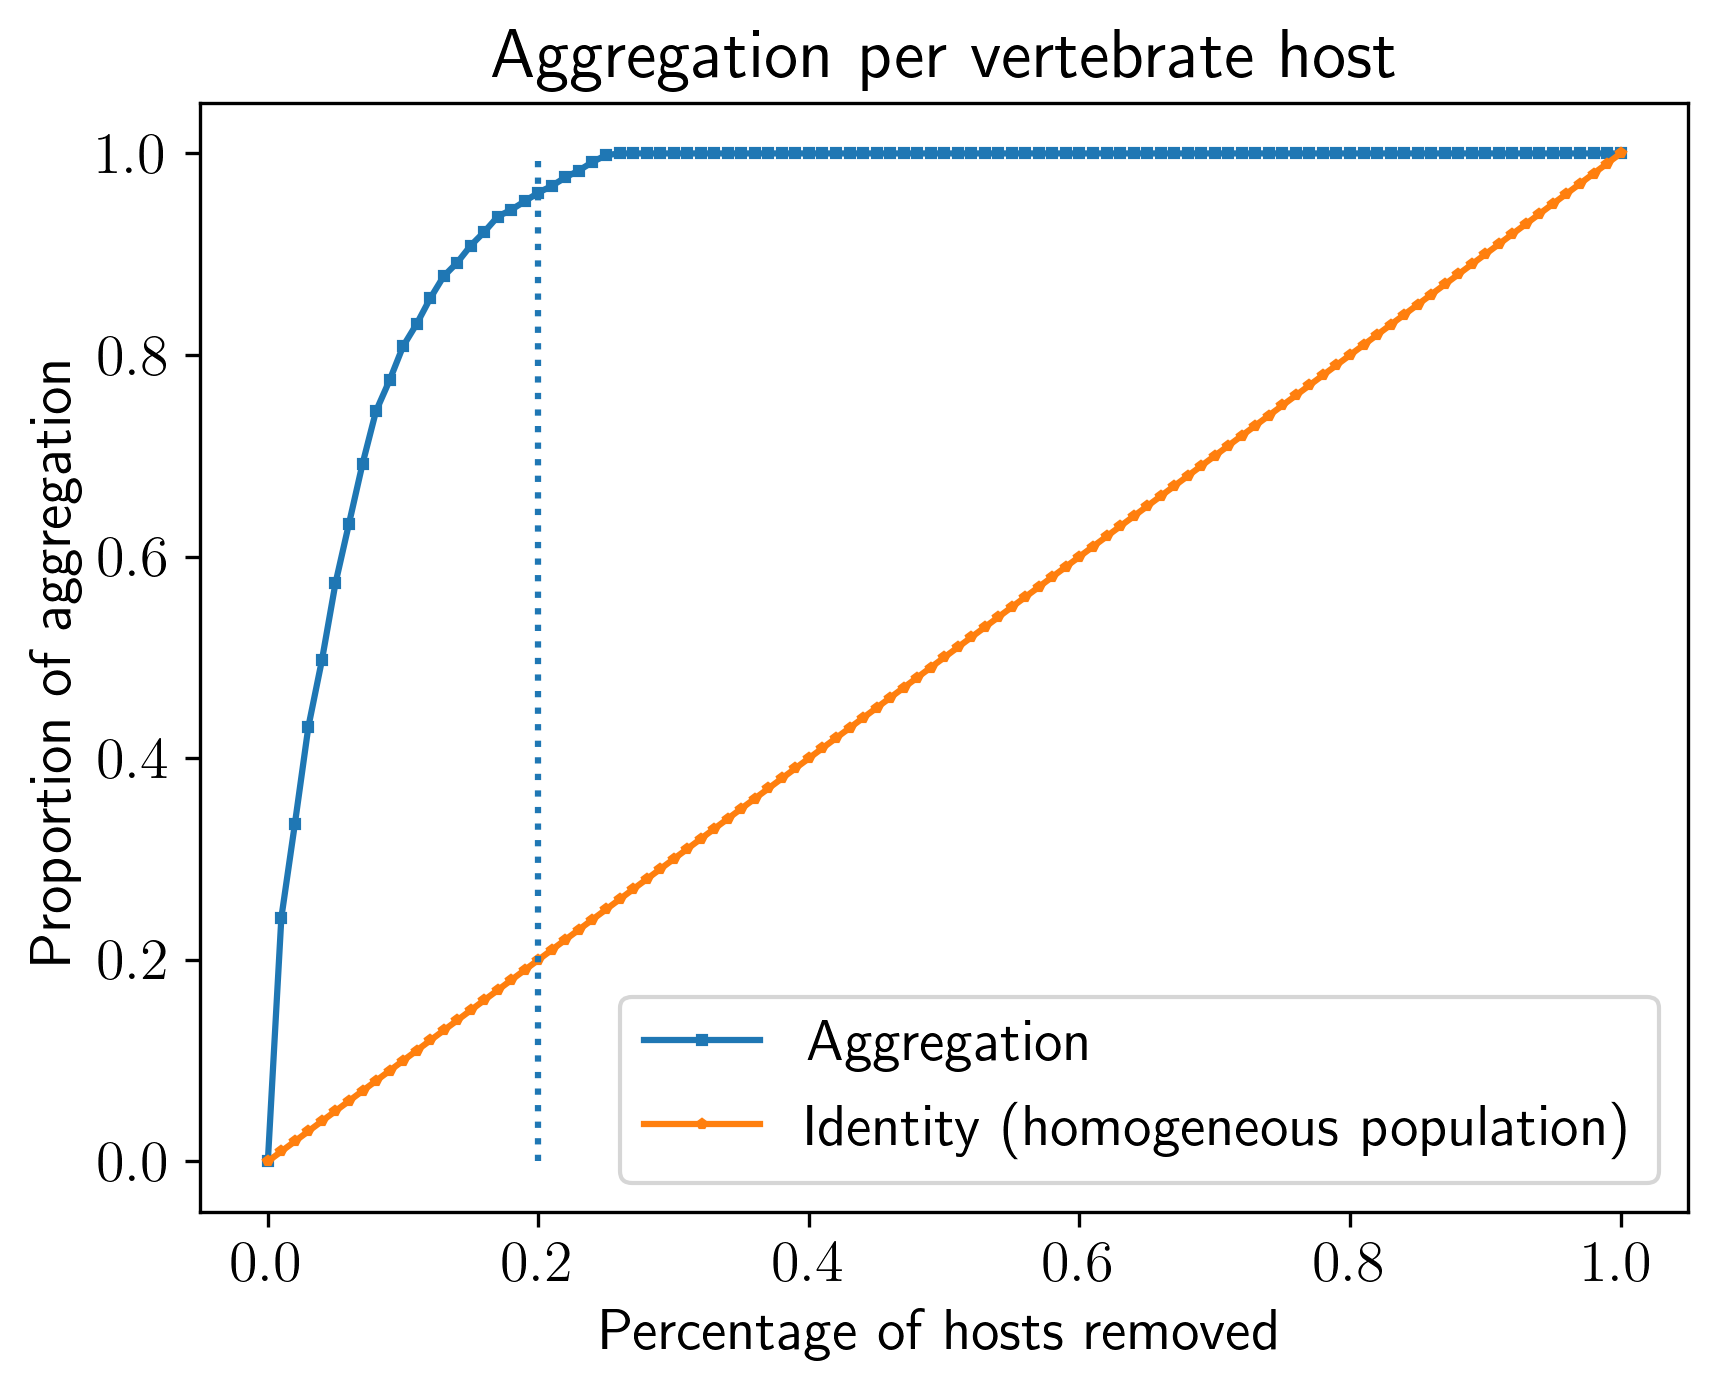
\includegraphics[width=.48\linewidth,valign=m]{lorenz_aggregation_SA_2005_I.Trianguliceps} & 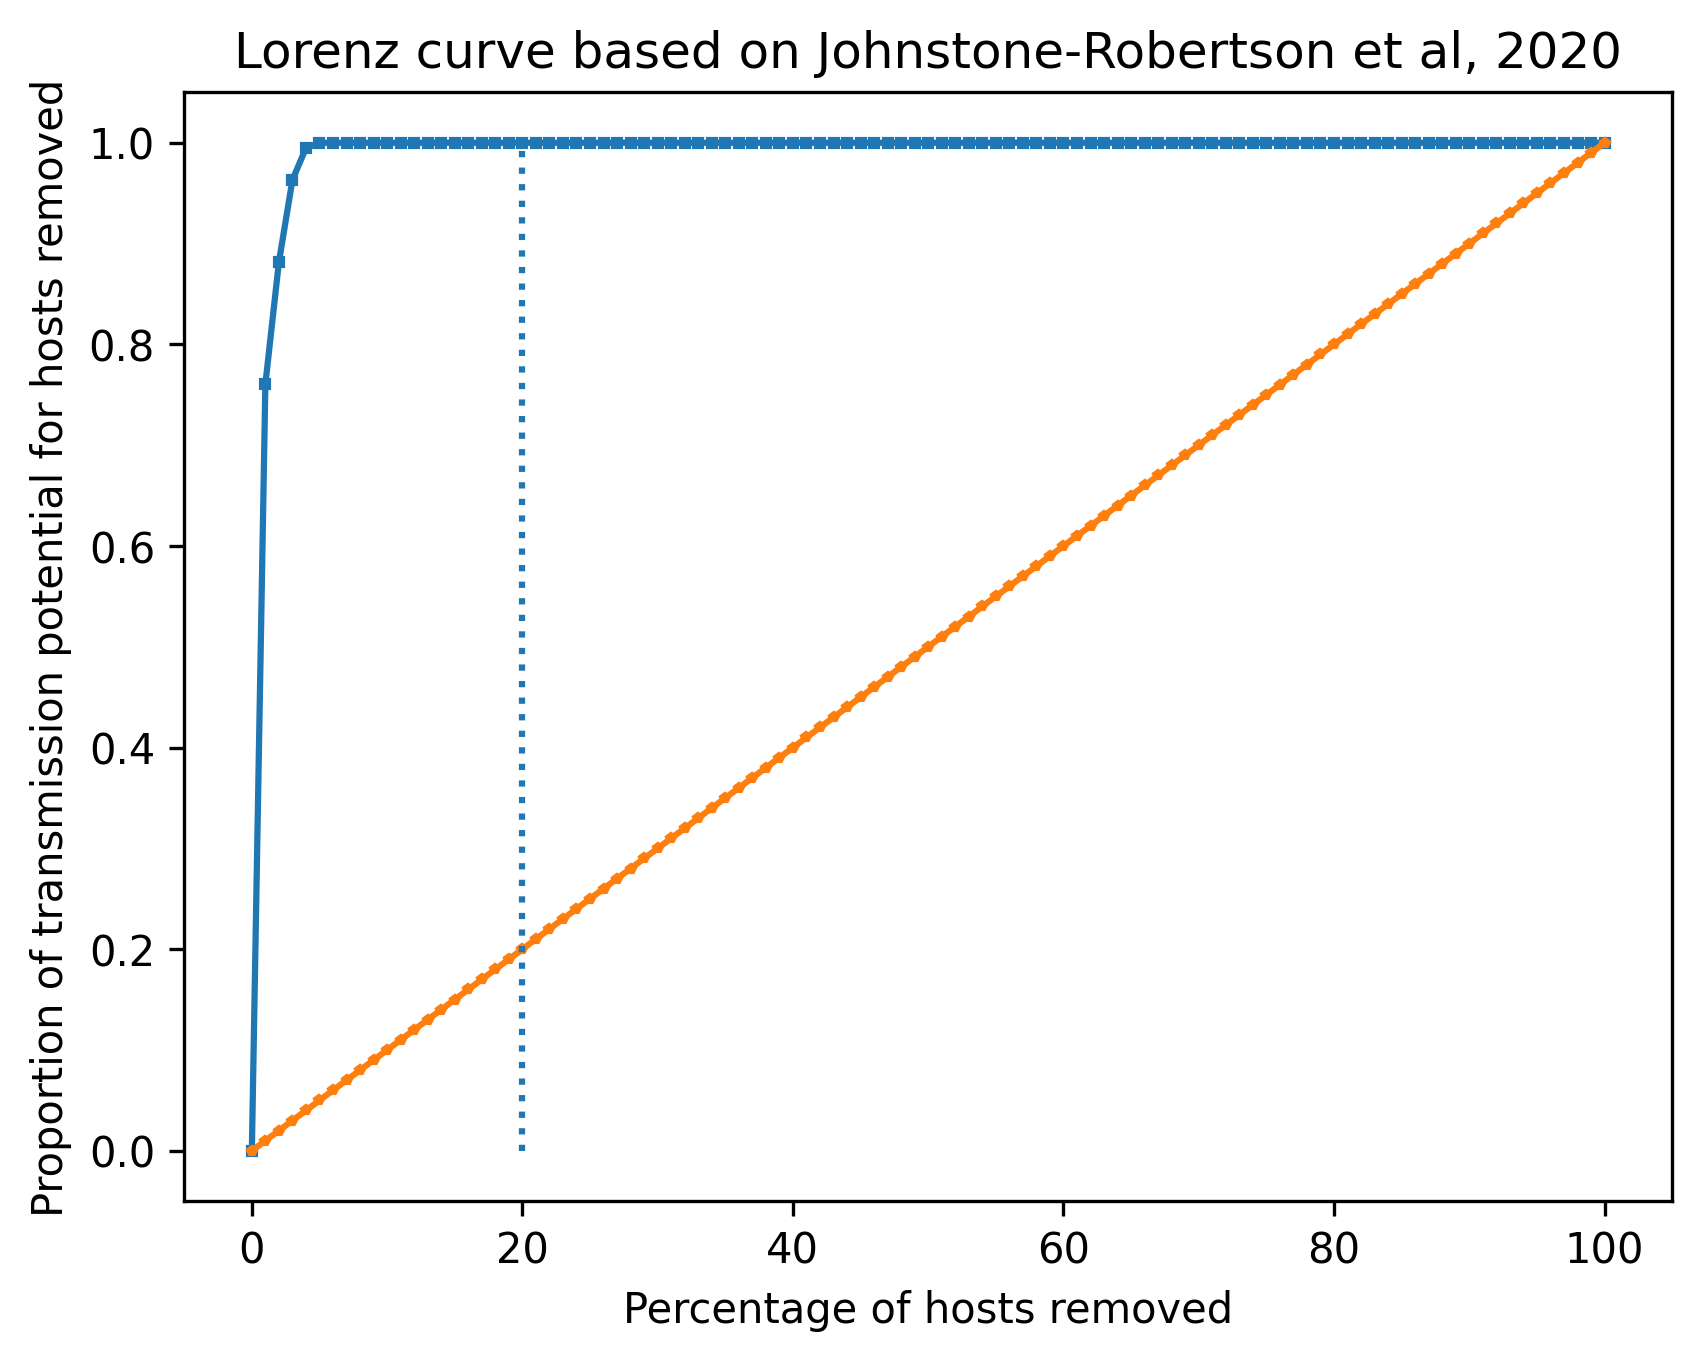
\includegraphics[width=.48\linewidth,valign=m]{lorenz_JR_SA_2005_I.Trianguliceps} \\
	\end{tabular}
	\caption{Aggregation (left) and cumulative transmission potential (right) of \textit{common shrews} that were found with \textit{I. trianguliceps} in \textit{2005} in the Kielder Forest data.}
	\label{fig:lorenz_2005_itrianguliceps_SA}
	\end{mdframed}
\end{figure}

\begin{figure}[]
	\begin{mdframed}[backgroundcolor=grey250,rightline=false,leftline=false,topline=false]
	\centering
	\begin{tabular}{ll}
		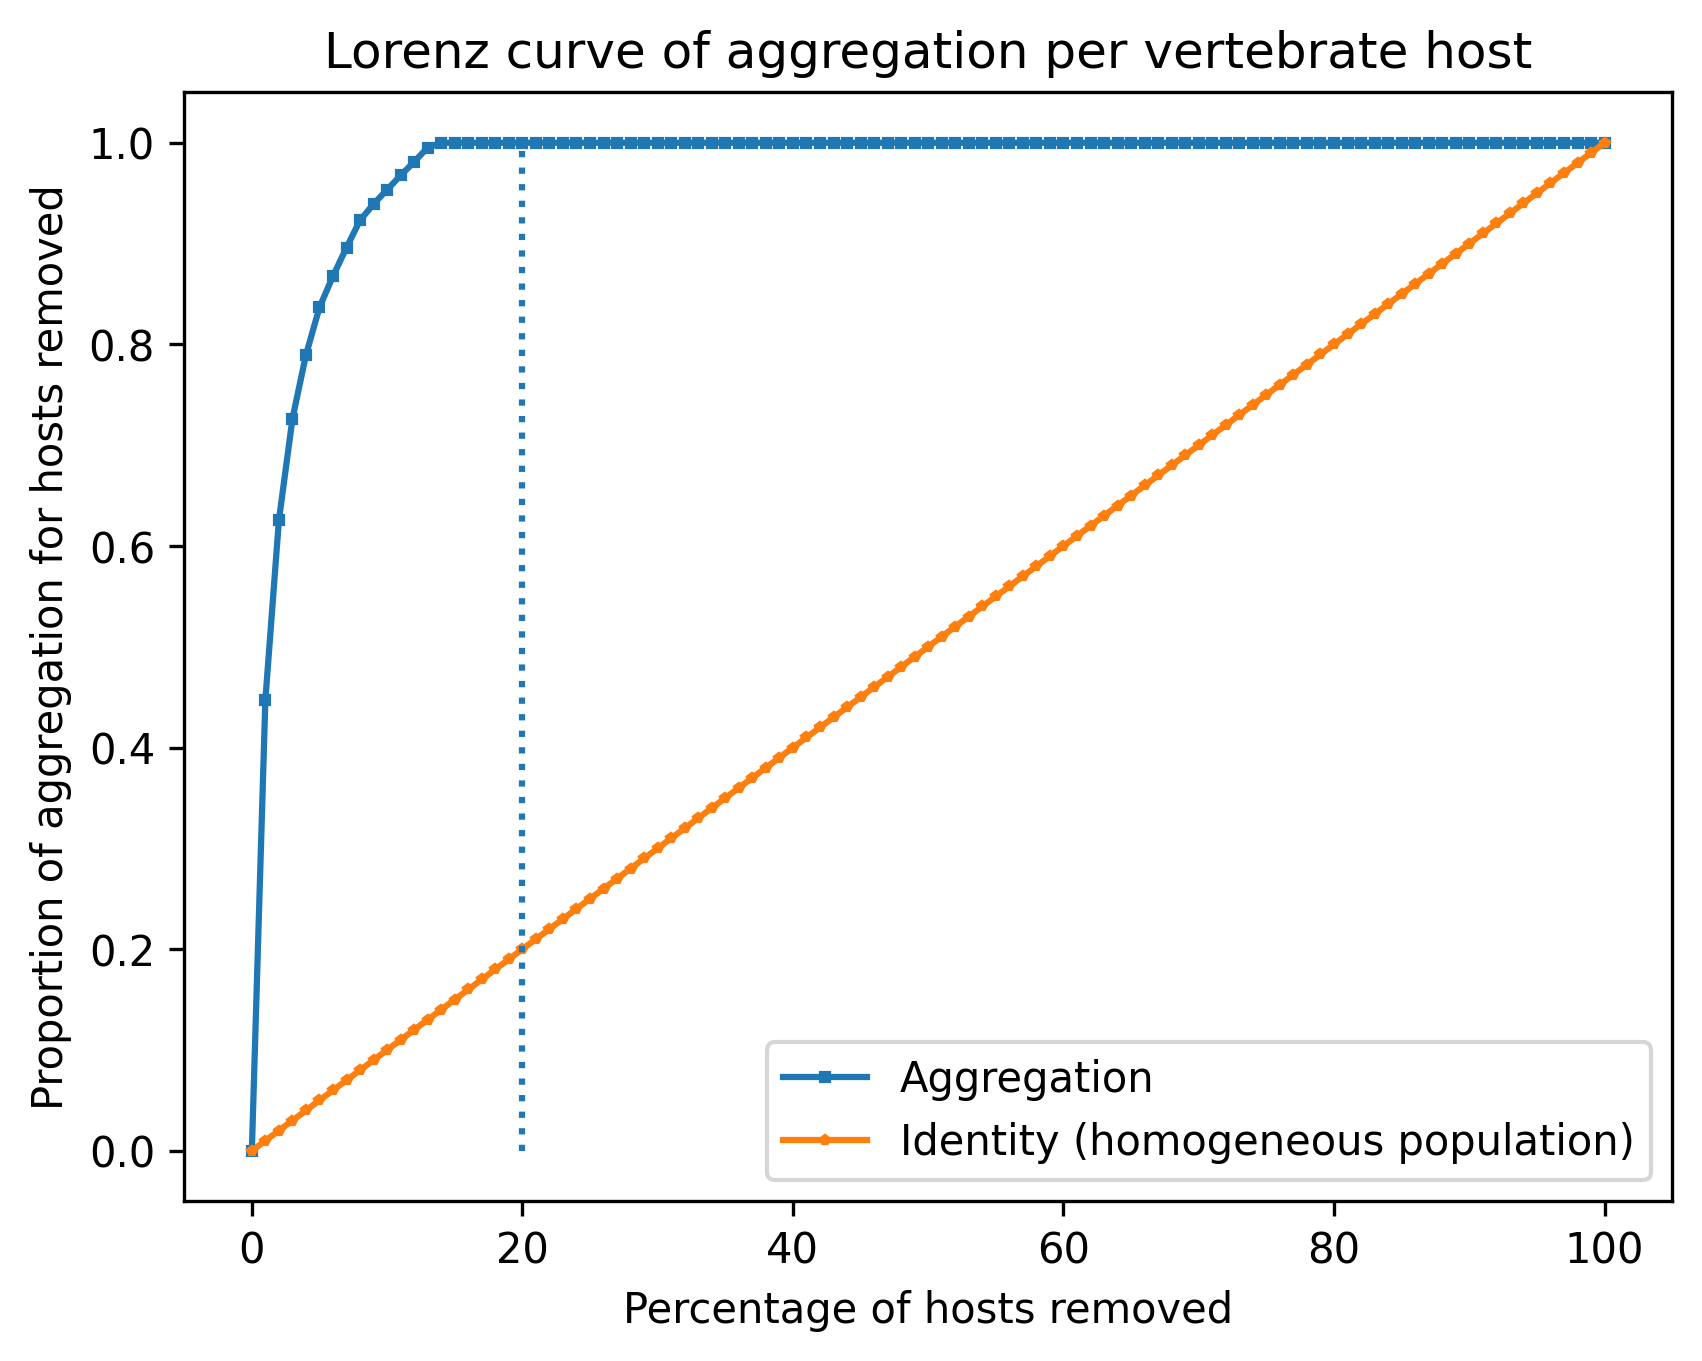
\includegraphics[width=.48\linewidth,valign=m]{lorenz_aggregation_FV_2005_I.Ricinus} & 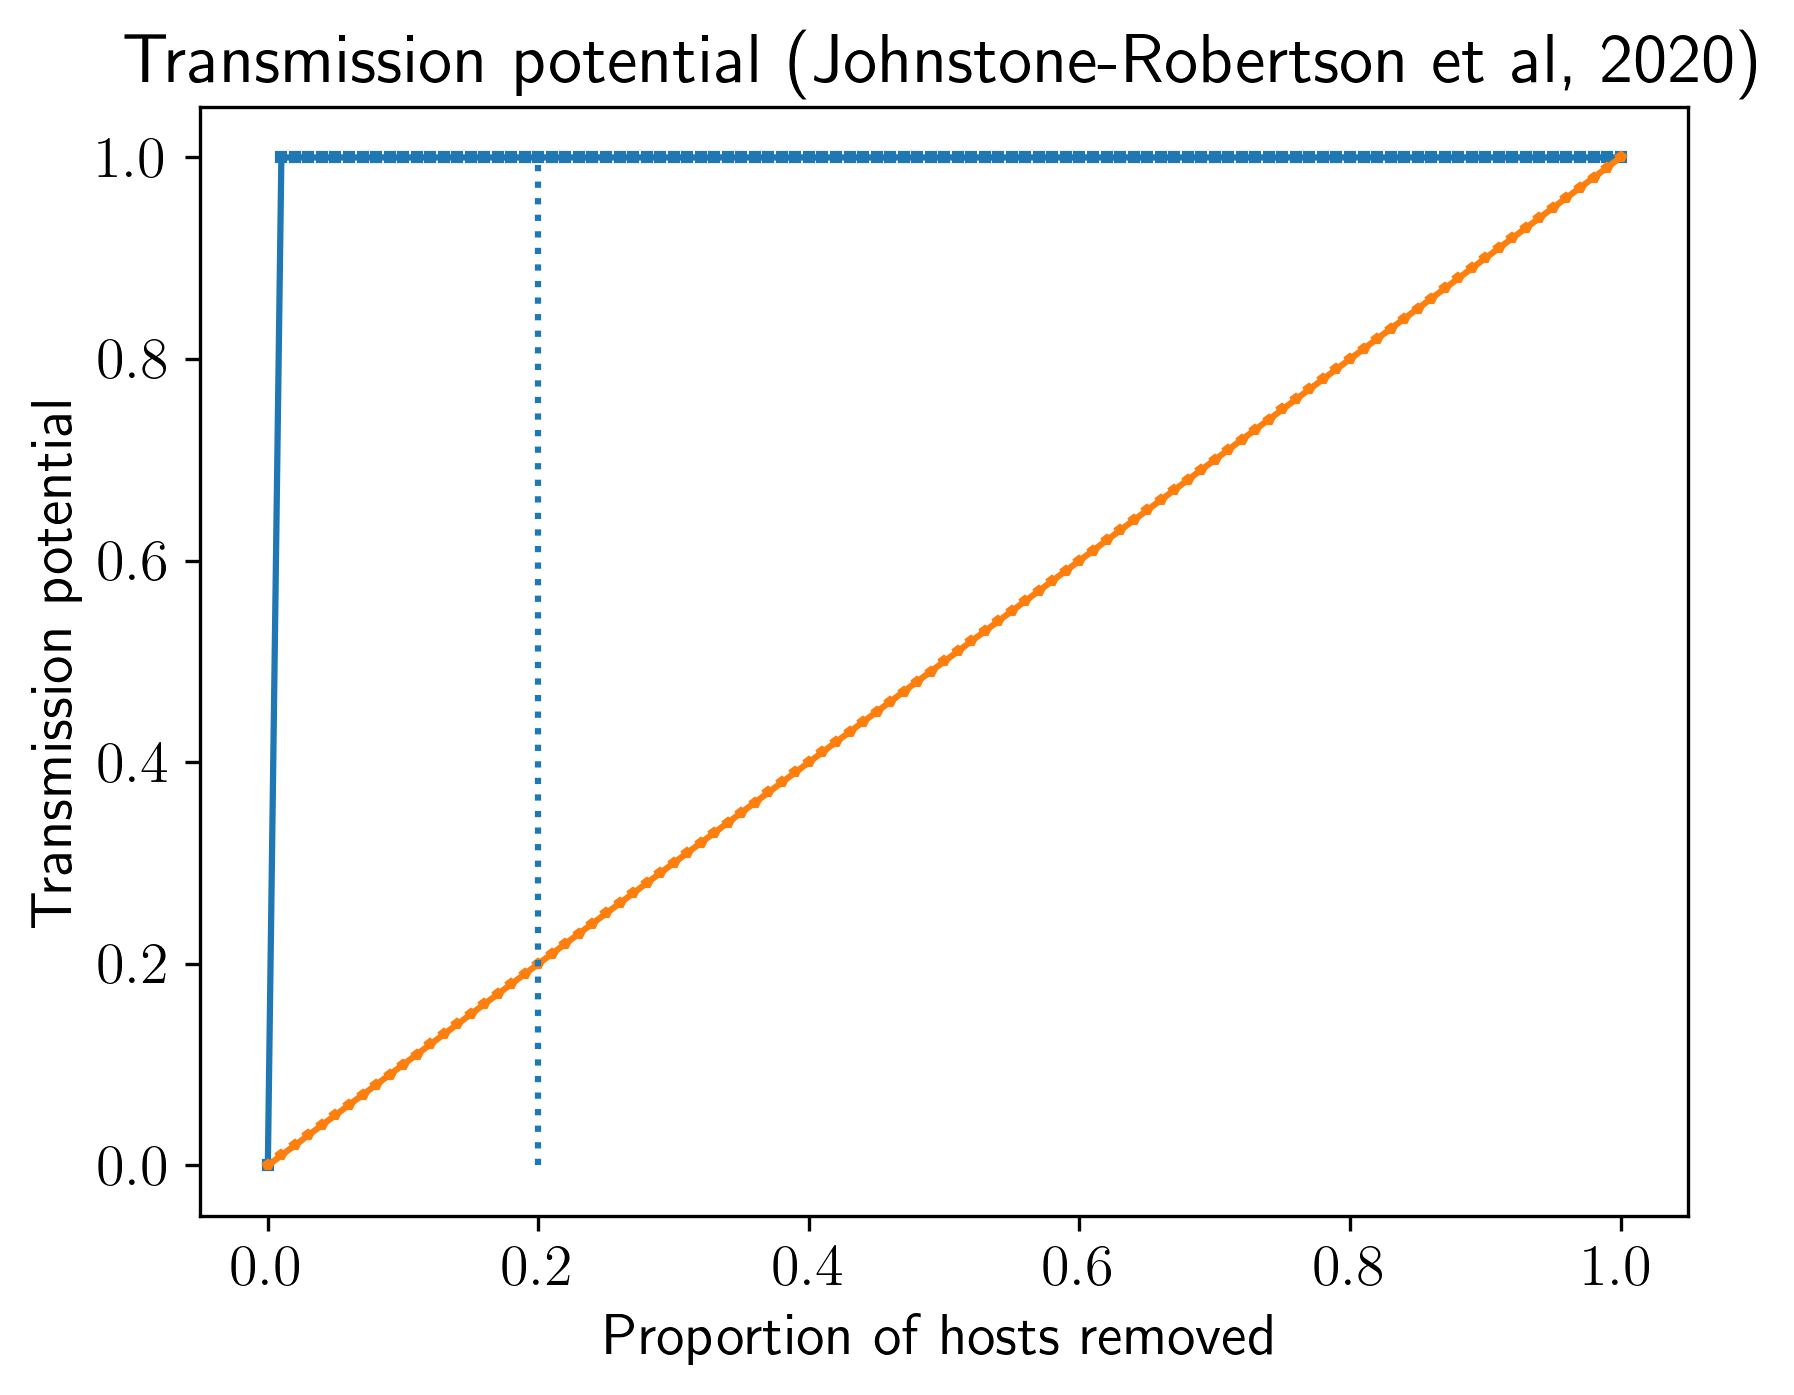
\includegraphics[width=.48\linewidth,valign=m]{lorenz_JR_FV_2005_I.Ricinus} \\
	\end{tabular}
	\caption{Aggregation (left) and cumulative transmission potential (right) of \textit{field voles} that were found with \textit{I. ricinus} in \textit{2005} in the Kielder Forest data.}
	\label{fig:lorenz_2005_iricinus_FV}
	\end{mdframed}
\end{figure}

\begin{figure}[]
	\begin{mdframed}[backgroundcolor=grey250,rightline=false,leftline=false,topline=false]
	\centering
	\begin{tabular}{ll}
		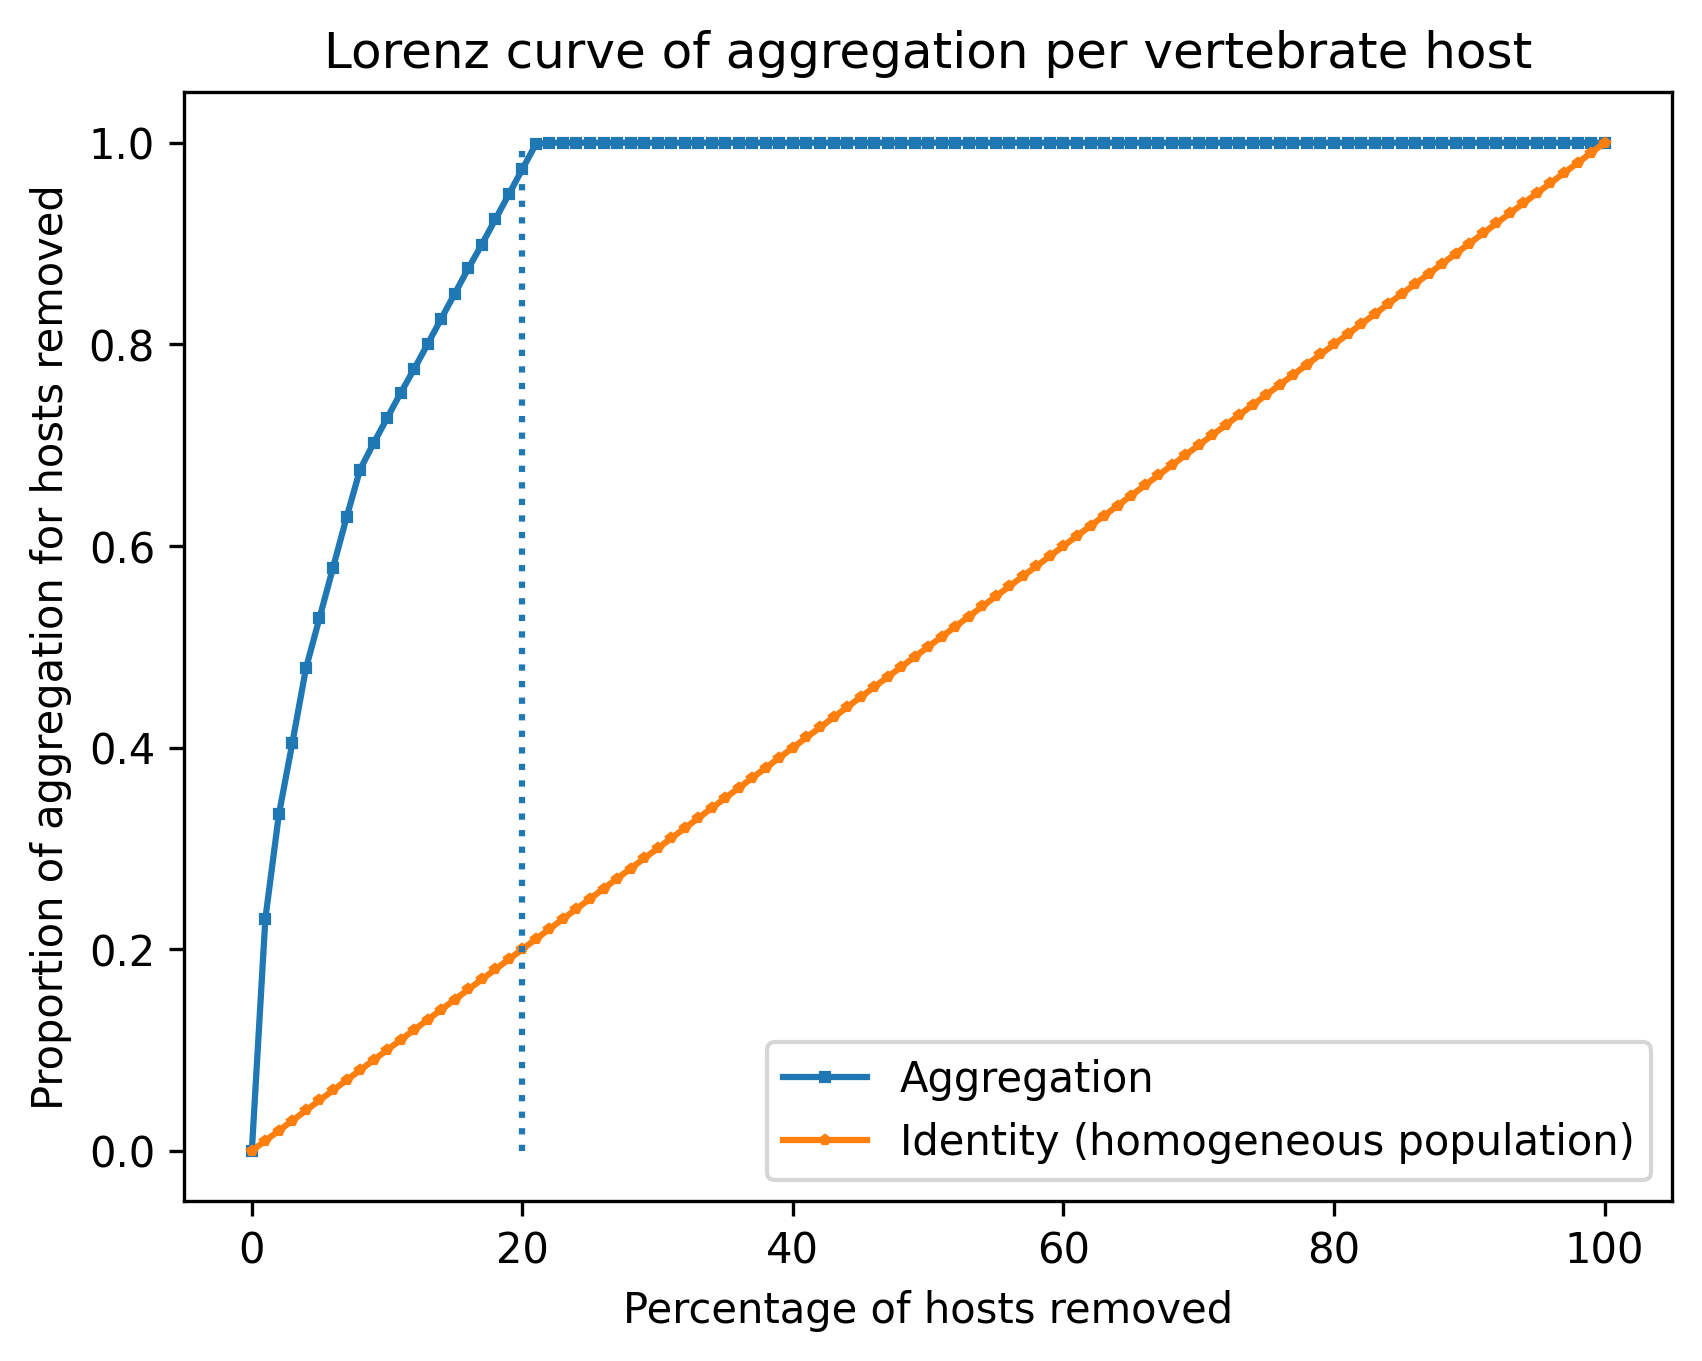
\includegraphics[width=.48\linewidth,valign=m]{lorenz_aggregation_FV_2005_I.Trianguliceps} & 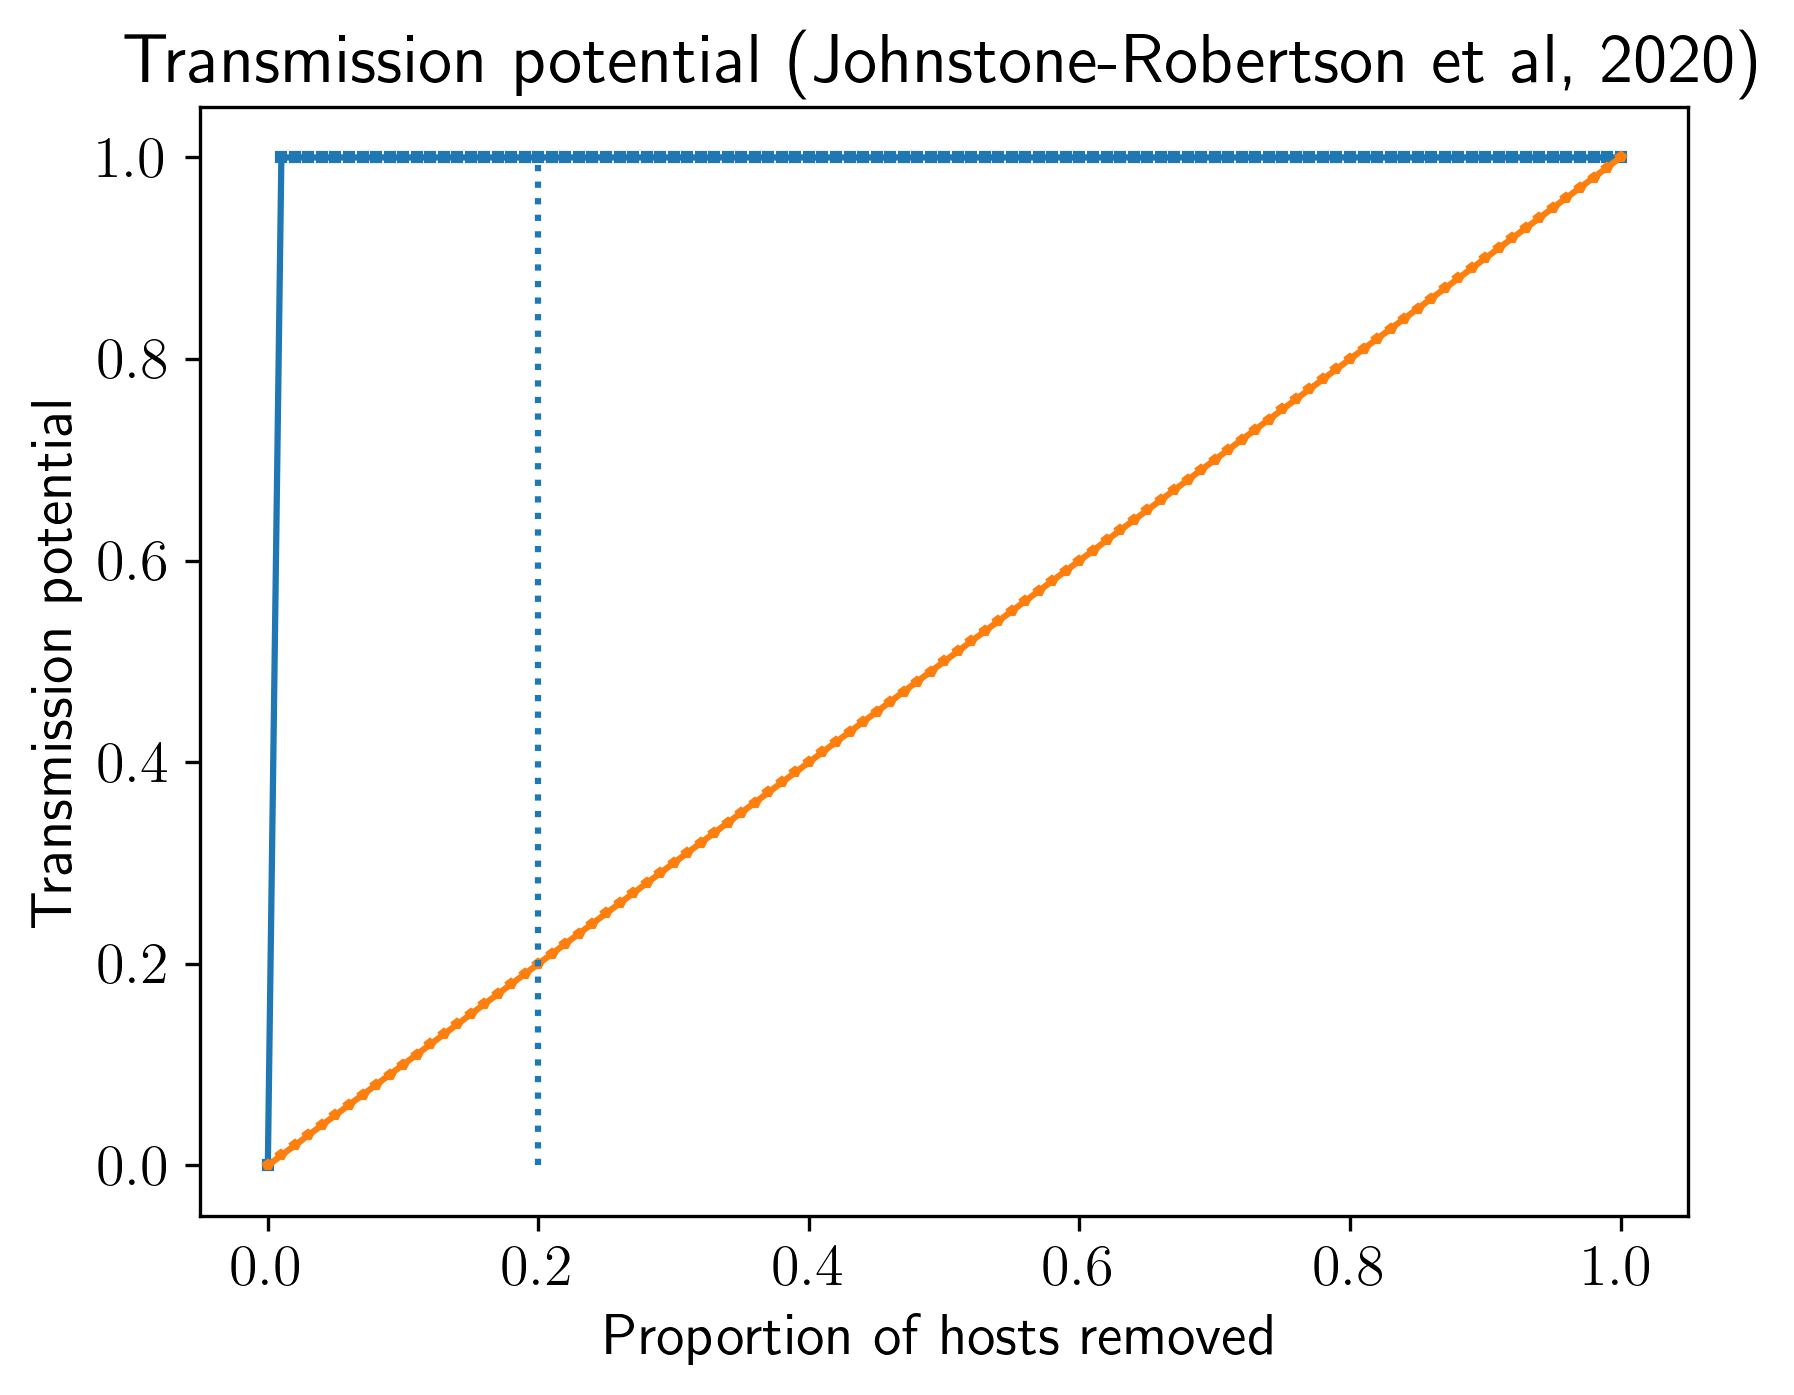
\includegraphics[width=.48\linewidth,valign=m]{lorenz_JR_FV_2005_I.Trianguliceps} \\
	\end{tabular}
	\caption{Aggregation (left) and cumulative transmission potential (right) of \textit{field voles} that were found with \textit{I. trianguliceps} in \textit{2005} in the Kielder Forest data.}
	\label{fig:lorenz_2005_itrianguliceps_FV}
	\end{mdframed}
\end{figure}

To find the Gini coefficient for each subset of data, we calculate the area between each Lorenz curve and the identity function. Since the identity function represents an idealised homogeneous population, where every vertebrate host has the same magnitude of tick immature burdens, then the Gini coefficient summarises the total amount of inequality present in the Kielder Forest data. 

As expected, aggregation counts follow the 80:20 rule somewhat, which is commonly reported for tick aggregation and parasite aggregation more generally \cite{}. Also as expected, co-feeding transmission potential is even more heterogeneous, which matches the finding by Perkins et al \cite{}. However, the heterogeneity for co-feeding transmission potentials in the Kielder Forest data is greater than the finding by Perkins et al: Figures \ref{fig:lorenz_2005_iricinus_FV} and \ref{fig:lorenz_2005_itrianguliceps_FV} show that just 1\% of vertebrate hosts were responsible for all transmission potential of field voles in 2005, for \textit{I.ricinus} and \textit{I.trianguliceps}.

\begin{table}[ht]
	\begin{mdframed}[backgroundcolor=grey250,rightline=false,leftline=false,topline=false]
	\centering
	\begin{tabular}{|l|l|l|r|r|}
		\hline
		\textbf{Tick species}     & \textbf{Host species} & \textbf{Year} & \multicolumn{1}{c|}{\textbf{Aggregation}} & \multicolumn{1}{c|}{\textbf{\begin{tabular}[c]{@{}c@{}}Transmission \\ potential\end{tabular}}} \\ \hline
		\textit{I. trianguliceps} & \textit{Common shrew} & 2004          & 0.747                                     & 0.963                                                                                           \\ \hline
		\textit{I. trianguliceps} & \textit{Common shrew} & 2005          & 0.885                                     & 0.984                                                                                           \\ \hline
		\textit{I. trianguliceps} & \textit{Field vole}   & 2005          & 0.869                                     & 0.993                                                                                           \\ \hline
		\textit{I. ricinus}       & \textit{Common shrew} & 2004          & 0.871                                     & 0.989                                                                                           \\ \hline
		\textit{I. ricinus}       & \textit{Field vole}   & 2005          & 0.95                                      & 0.993                                                                                           \\ \hline
	\end{tabular}
	\caption{Gini coefficients for each of the five subsets of data, for total counts of immature tick aggregation (left) and for co-feeding transmission potentials (right), both derived from larval burdens collected in the Kielder Forest.}
	\label{tab:kielderGINI}
	\end{mdframed}
\end{table}

\clearpage

\section{Reproducing the results by Lloyd-Smith et al, 2005}

Before we follow the example set by Lloyd-Smith et al \cite{LloydSmith2005}, it will be useful to re-implement parts of their work. Their work included using a stochastic simulation of pathogen transmissions, and numerical approximation to predict the probability that a chain of transmissions becomes extinct, for some pathogen and population with $ R_0, k $ that could be determined. They also used many interesting visualisations, which we can make use of later in this project.

Figures \ref{fig:gamma(R0,R0/k)}, \ref{fig:probabilityOfExtinction}, \ref{fig:firstGenerationToReach100Offspring} are reproduced versions of the charts shared by Lloyd-Smith et al. These illustrate the effect of individual reproductive number $ v $. A link to the code to generate these charts is shared in the appendix. To produce each chart, when $ k = \infty $, we used $ 10^b $ where $ b $ is the largest integer such that $ 10^b $ did not produce numerical errors.

Figure \ref{fig:firstGenerationToReach100Offspring} highlights the effect of superspreaders. We first use a stochastic simulation that randomly draws the individual reproductive number $ v $ from the $ Gamma\left(R_0, \frac{R_0}{k}\right) $ distribution. Then numbers of offspring are randomly drawn from a Poisson Mixture: $ Poisson(v) $. That means there are two sources of randomness in the simulations presented in Figure \ref{fig:firstGenerationToReach100Offspring}. We record the number of generations required before a generation with 100 offspring is found. We also record the rate of outbreaks that survive 10,000 generations. A low value for $ k $ implies a heterogeneous population where few individuals infect many others. Inversely, $ k = \infty $ implies a homogeneous population where each individual infects (close to) $ R_0 $ others. For low values of $ k $, the related low survival rate (along the second vertical axis) combined with the smaller average and smaller spread in the number of generations before a generation with 100 offspring is found, indicates that when $ k $ is small an outbreak either explodes in numbers quickly or not at all.

By comparing Figures \ref{fig:probabilityOfExtinction} and \ref{fig:firstGenerationToReach100Offspring}, we can see that when $ R_0=1.5 $, then the extinction probability $ q $ is roughly the complement of the survival rate. That is not surprising, but it is interesting and encouraging to see.

\begin{figure}[]
	\begin{mdframed}[backgroundcolor=grey250,rightline=false,leftline=false,topline=false]
    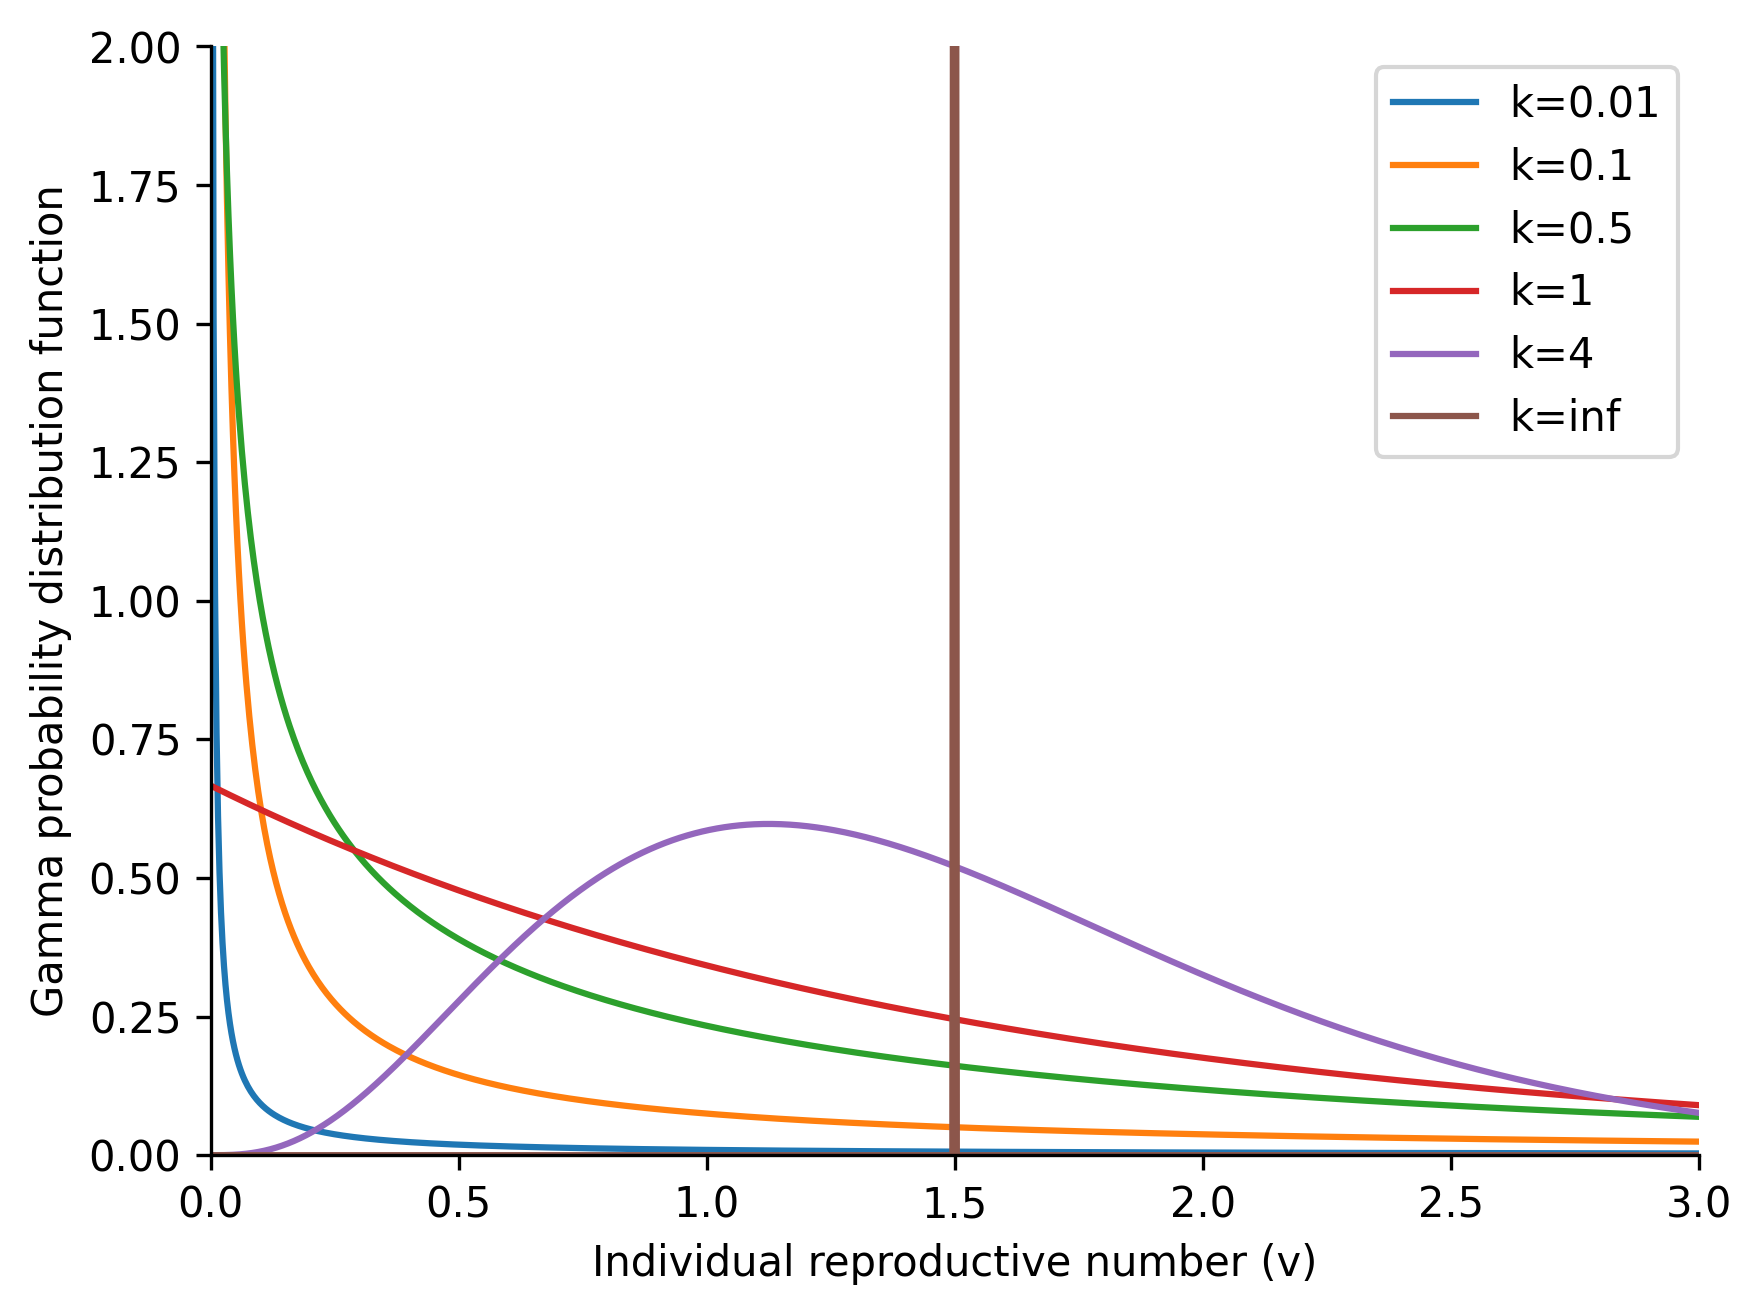
\includegraphics[width=0.48\textwidth, center]{2a_gamma.png}
    \caption{The individual reproductive number $ v \sim \text{Gamma}(R_0, \frac{R_0}{k}) $. This chart shows the effect of fixing $ R_0=1.5 $ and allowing $ k $ to vary. Note that for $ k = \infty $, we used $ k=10^7 $.}
    \label{fig:gamma(R0,R0/k)}
	\end{mdframed}
\end{figure}

\begin{figure}[]
	\begin{mdframed}[backgroundcolor=grey250,rightline=false,leftline=false,topline=false]
    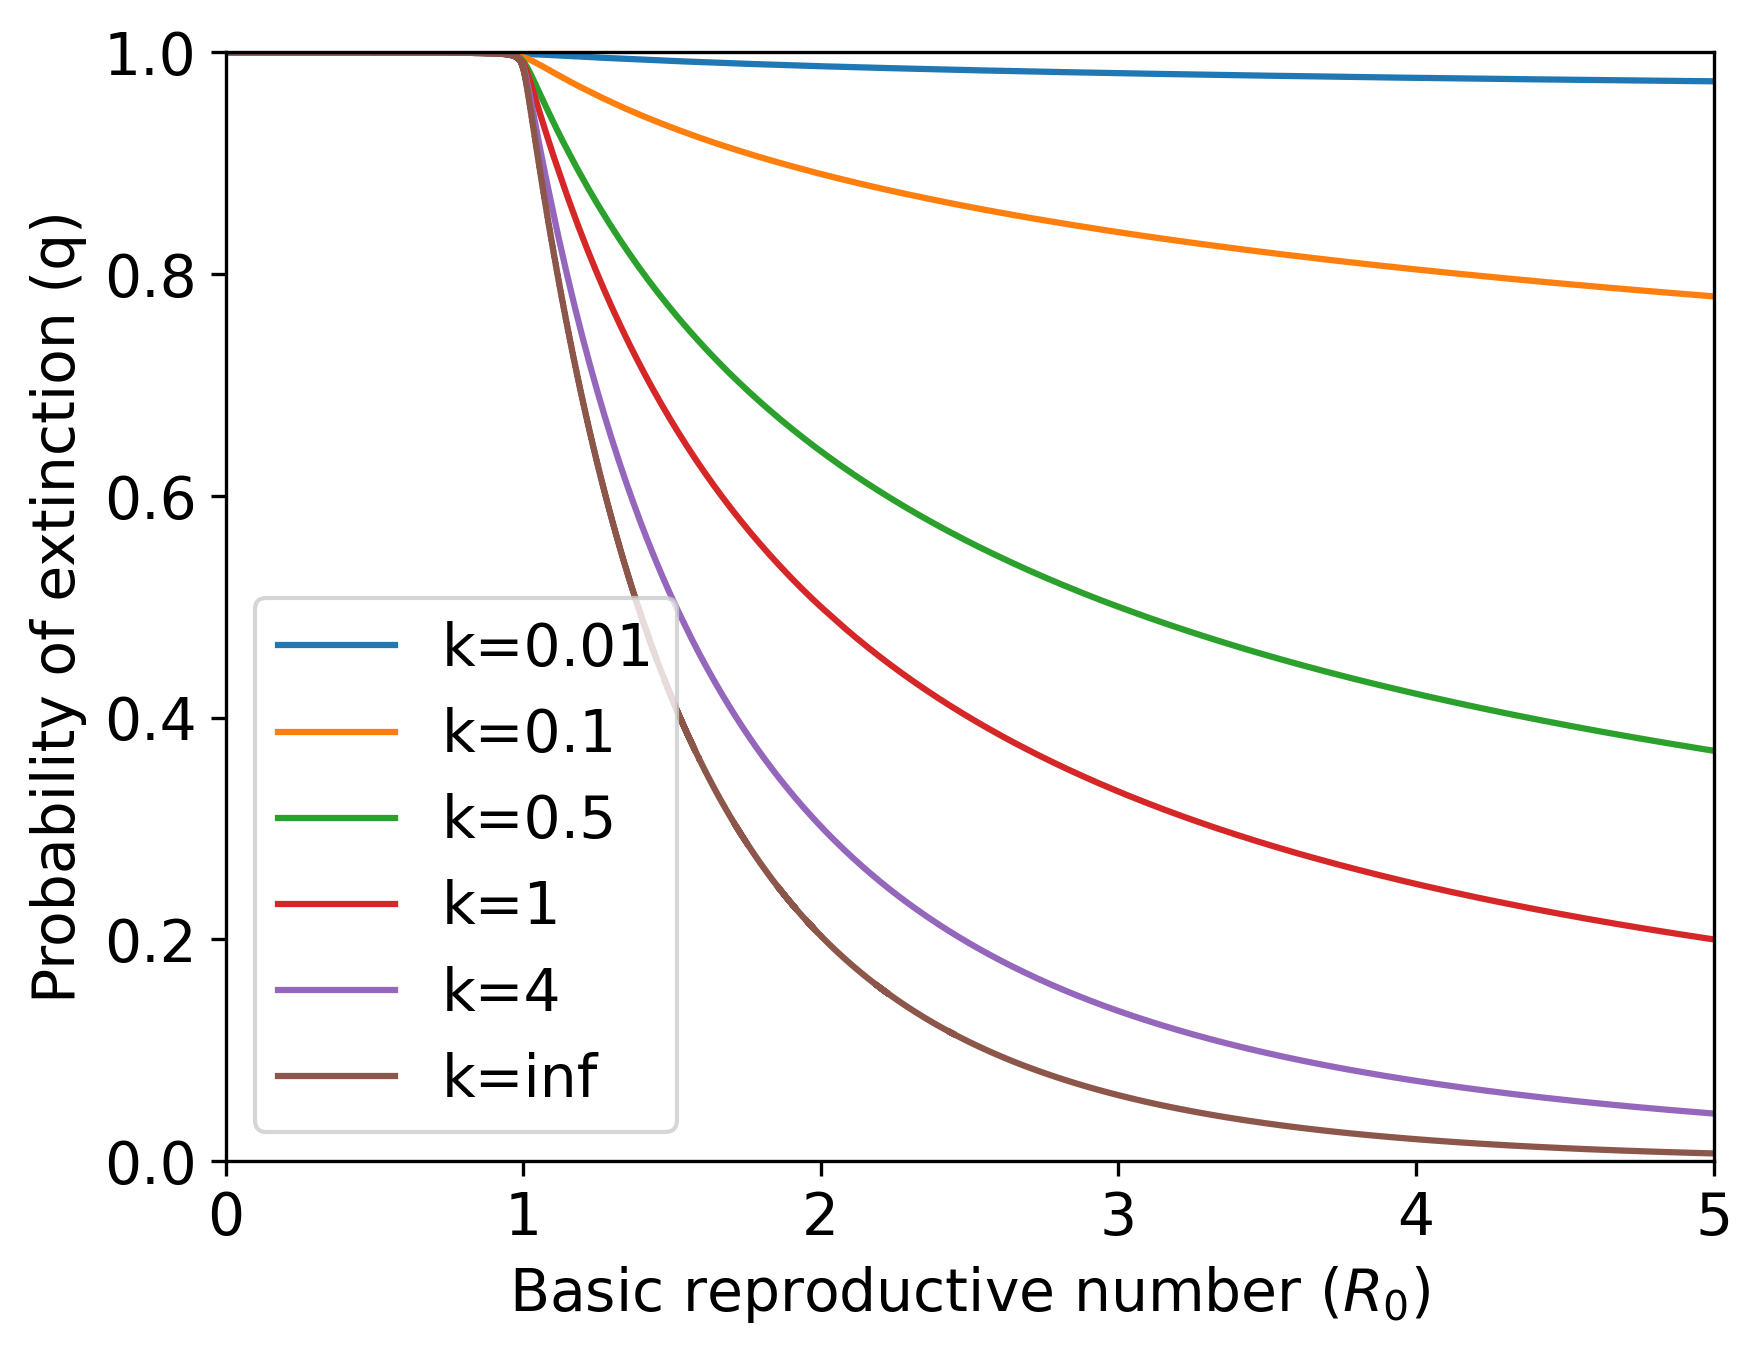
\includegraphics[width=0.48\textwidth, center]{2b_probabilityOfExtinction.png}
    \caption{If $ Z \sim \text{Poisson}(v) $, then the resulting Poisson Mixture is a negative binomial distribution, which is a candidate offspring distribution. The probability that a chain of transmissions becomes extinct for a combination of $R_0$ and $ k $, after the introduction of a single infected individual, is found by fixed point iteration over the negative binomial distribution's probability generating function. Each simulation generates a random value for $ v \sim \text{Gamma}(R_0, \frac{R_0}{k})$. Note that for $ k = \infty $, we used $ k=10^{12} $. The vertical dotted line is $ R_0=1.5$ that we use in Figure \ref{fig:firstGenerationToReach100Offspring}.}
    \label{fig:probabilityOfExtinction}
	\end{mdframed}
\end{figure}

\begin{figure}[]
	\begin{mdframed}[backgroundcolor=grey250,rightline=false,leftline=false,topline=false]
    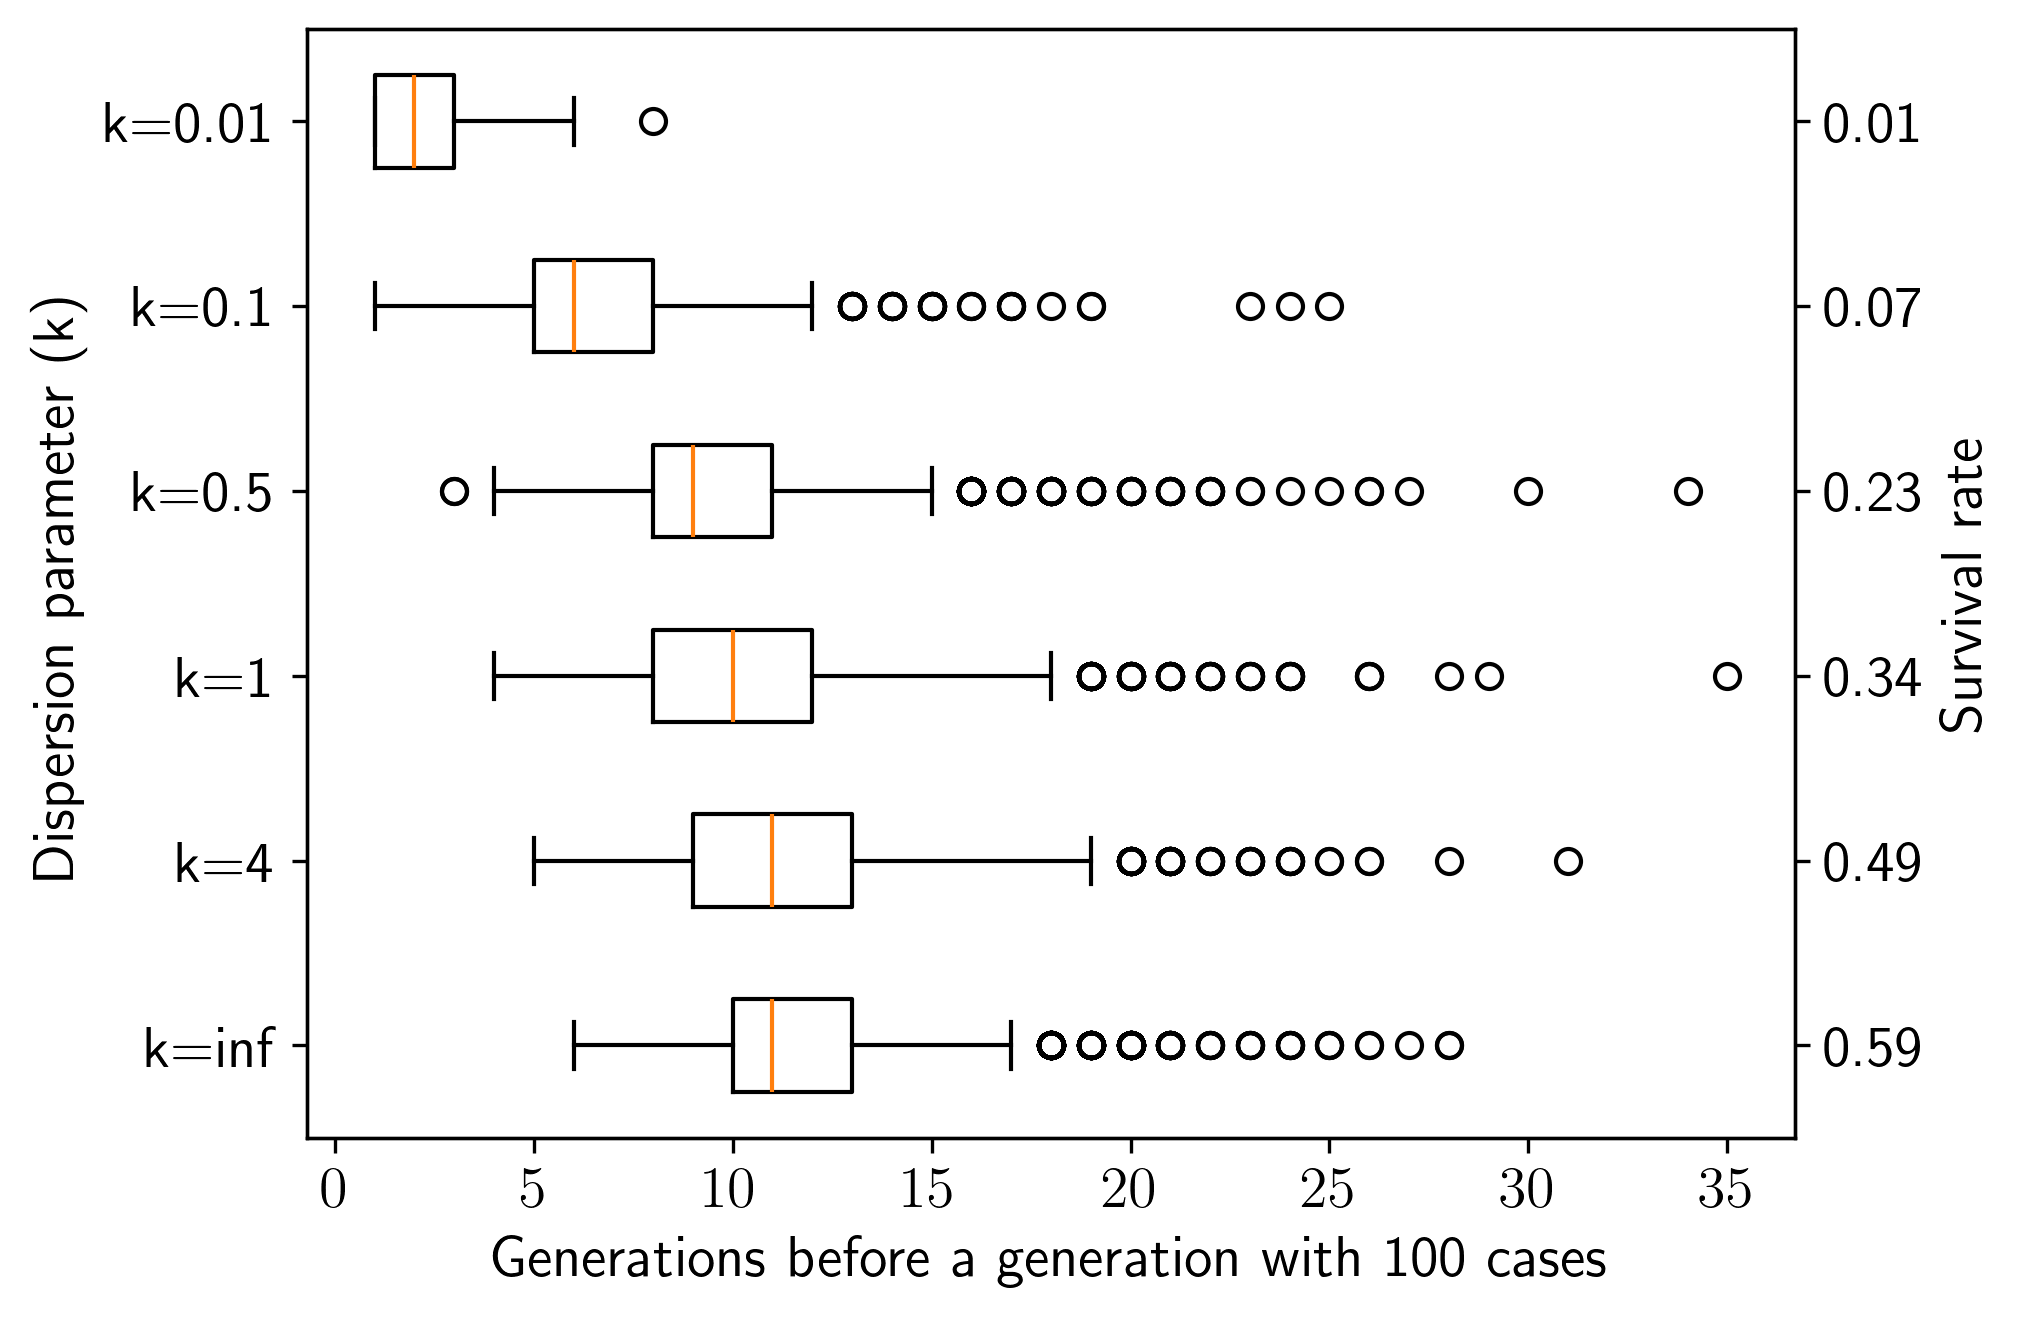
\includegraphics[width=0.48\textwidth, center]{2c_firstGenerationReach100Offspring.png}
    \caption{Lloyd-Smith et al used a simulation, with the first generation to reach 100 offspring used as an arbitrary benchmark. Boxes represent the interquartile ranges for how many generations were required before a single generation contained 100 offspring, given different values of $ k $ and a fixed $ R_0=1.5 $. Note that for $ k = \infty $, we used $ k=10^7 $. The values along the right vertical axis are the proportion of outbreaks that survived 10,000 generations.}
    \label{fig:firstGenerationToReach100Offspring}
	\end{mdframed}
\end{figure}

Lloyd-Smith et al noted that if $ v \sim \text{Gamma} $ and if there is a Poisson mixture $ Z \sim \text{Poisson}(v) $, then that Poisson mixture simplifies to a negative binomial distribution. If $ Z $ is also the offspring distribution of a GWBP, then we can use the probability generating function of that negative binomial distribution to approximate the probability that a chain of transmissions becomes extinct. By first reparameterising the negative binomial distribution, we can express the probability generating function (as Lloyd-Smith et al did) in terms of $ R_0, k $. The derivation for that particular probability generating function is presented in \eqref{NegBinom_PGF}. By using the more general result of convergence presented in \eqref{BranchingProcessRecurrence}, we can approximate the probability of extinction by fixed point iteration, which is the process that Figure \ref{fig:probabilityOfExtinction} shows for different combinations of $ R_0, k $.

In this honours project we use count data of larvae per nymph. Before we can find the offspring distribution's parameters $ R_0 $ and $ k $, for use in a branching process analysis, we must introduce a method to derive a transmission network from the larval count data. For our purposes, $ v $ is already represented in the larval count data. We also test the negative binomial distribution is a good fit to the data.

\newpage

\section{Reparameterisation of the negative binomial distribution}

While the work by Lloyd-Smith et al, presented above, uses the negative binomial distribution, it remains to be seen that it is the best fit for our tick larval count data. To test it, we first need to derive the same parameterisation that Lloyd-Smith et al used. Then, it will be a candidate for the offspring distribution. Other candidate discrete distributions are the Poisson and geometric distributions; later in this project, we fit all distributions to the same data and then compare goodness-of-fit for each.

Commonly, the negative binomial distribution is presented as:

\begin{equation}\label{NegBinom}
	Z \sim NB(x | p, k) = \left(\begin{matrix}x+k-1 \\ x \end{matrix}\right) \space p^k q^x, \space \space \space \space \space x \in \mathbb{N}
\end{equation}

But, a more convenient parameterisation uses the sample mean $ m $ and dispersion parameter $ k $ as parameters \cite{Rice2007}. This is possible with $ p = \frac{k}{m+k} $:

\begin{equation}\label{NegBinomReparam}
    Z \sim NB(x | m, k) = \frac{\Gamma(x+k)}{x!\Gamma(k)} \space \left(1+\frac{m}{k}\right)^{-k} \space \left(\frac{m}{m+k}\right)^x, \space \space \space \space \space x \in \mathbb{N}
\end{equation}

Before fitting the distribution to some data the sample mean $ m $ can already be found from the data itself. Finding the dispersion parameter $ k $ is achievable with maximum likelihood estimation (MLE). Since the parameters $ m, k $ have asymptotically orthogonal limits \cite{LloydSmith2005}, then we can find $ k $ via MLE without doing so for $ m $, which is useful since $ m $ is known.

Lloyd-Smith et al fit the reparameterised negative binomial distribution to contact trace data, where the sample mean for each dataset is $ m=R_0 $. An important nuance is that to find $ R_0 $ from counts of larvae per nymph, since we do not have contact trace data, another step is required to account for stochasticity in transmission. In this thesis $ m $ is the sample mean of larvae per nymph counts and $ m \ne R_0 $, but we derive an expression for finding $ R_0 $ in a later section.

In this project, we tested the standard negative binomial distribution, available in Python's Scipy package, against the reparameterisation \eqref{NegBinomReparam} by fitting both distributions to the same data. Results indicate a similar fit. A link to the code is available in the appendix.

Below, we derive the probability generating function for the negative binomial distribution \eqref{NegBinom}, and then perform a change of variables, as in \eqref{NegBinomReparam}. Note the definition of a probability generating function given in \eqref{BranchingProcessPGF} is employed below.

\begin{align}
	g(z) &= \sum_{x=0} \left(\begin{matrix}x+k-1 \\ x  \end{matrix}\right) \space p^k q^x z^x \nonumber \\ 
	     &= p^k \sum_{x=0} \left(\begin{matrix}x+k-1 \\ x \end{matrix}\right) \space (qz)^x \nonumber \\
	     &= p^k (1-qz)^{-k} \label{NegBinomTheorem} \\
	     &= \left(\frac{k}{m+k}\right)^k \left(1-\frac{m}{m+k}z\right)^{-k} \nonumber \\ 
	     &= \left(1 + \frac{m}{k}(1-z)\right)^{-k} \label{NegBinom_PGF}
\end{align}

Above, \eqref{NegBinomTheorem} is a result of the negative binomial theorem. The equation on line (\ref{NegBinom_PGF}) is the final form of the probability generating function, for use with numerical approximation later in this project.

\newpage

\section{Determining the offspring distribution's parameters}

Given the scenario where a single infected tick is introduced to a population of vertebrate hosts for the first time, there is no guarantee that the tick will infect any other tick. Even if it did, those infected ticks might not infect any others for a number of reasons. There is no reason to think that all ticks will share the same individual reproductive number $ v $. Deterministic compartment models are not appropriate for estimating the probability that a chain of transmissions in a TBD network becomes extinct in the first stages of an outbreak due to their underlying assumption of homogeneous populations in each compartment. Since the infected compartment in such a model must be small at the start of an outbreak, then that compartment can not be said to be homogeneous in any meaningful way.

To calculate the probability that a chain of TBD transmissions becomes extinct, we can use a single-type GWBP analysis similar to the example set by Lloyd-Smith and others used in their 2005 paper \cite{LloydSmith2005}. To do that, however, we first require a candidate for the offspring distribution.

\subsection{A process to find parameters \texorpdfstring{$ R_0 $}{R0} and \texorpdfstring{$ k $}{k}}

Lloyd-Smith and others estimated $ R_0 $ and then found an estimate for $ k $ by using contact-tracing network data. In our case, we do not have contact-trace data. We instead have empirical data for the co-aggregation of larvae and nymphs on individual vertebrate hosts and co-aggregation does not mean that each pair of larva and nymph was a transmission. Instead, we can use a stochastic process to simulate a transmission network based on the empirical data in the sense that each pair of co-feeding larva and nymph is a potential transmission.

Let us note some characteristics of diseases where \textit{Ixodidae} tick species are the vectors:
\begin{itemize}
	\item Since an \textit{Ixodidae} larva will take one blood meal before it moults into a nymph, then the only way for an that larva to be infectious when it takes its blood meal would be if it was already infected via transovarial transmission.
	\item Given that ticks die during and between their life stages, then larvae will be relatively common, nymphs less common, and adults less common still \cite{Randolph1998}.
	\item Adult ticks tend to feed on larger vertebrates, whereas immature ticks (larvae and nymphs) frequently feed on small vertebrate hosts \cite{Herrmann2015, Randolph1998}.
	\item Since immature ticks prefer to feed on smaller vertebrate hosts, then they are more likely to feed in close proximity.
	\item Nymph-to-nymph co-feeding transmission is rare \cite{VOORDOUW2014}.
\end{itemize}

So, if a TBD was to spread through a population of ticks via co-feeding transmission, in the absence of transovarial and systemic transmission, then the majority of infections would pass from nymphs to larvae. Each larva would need to moult into a nymph and then successfully find another host before it could then pass the pathogen onto larvae that it co-aggregates with. During moulting the pathogen would need to survive transstadially as each infected larva becomes an infectious nymph. The ticks that co-aggregate would need to feed close enough for the transmission to occur.

Then, let us introduce these terms:

\begin{description}[leftmargin=1cm, style=nextline]
    \item[$ c $] be the contact rate, or the probability that a larva and infectious nymph co-feed close enough for transmission to occur.
    \item[$ v $] be the probability of transmission, since individual variation means not every infectious nymph has the same capability to transmit the disease.
    \item[$ \sigma $] be the probability that a larvae survives to become a nymph (moulting success).
    \item[$ \tau $] be the probability that transstadial transmission occurs.
\end{description}

Then for each larvae that co-feeds with an infectious nymph, the probability that it becomes an infectious nymph is found by:

\begin{equation} \label{alphaDef}
    \alpha = c v \sigma \tau
\end{equation}

$ \alpha $ will depend on the species of tick, the pathogen being transmitted, the vertebrate host ticks feed on, seasonal variation and perhaps other factors.

The network thinking by Johnstone-Robertson et al, in their 2020 paper \cite{JohnstoneRobertson2020}, is important for this project. Their superimposition of tick-to-tick transmission onto the tick-host contact network is the inspiration for the following idea: we can use count data of larvae per nymph to generate a nymph-larvae contact network for each nymph. The definitions below are placed into context in Figure \ref{fig:coaggregation_diagram}, which serves as a visual aide in understanding how we intend to find estimates for $ R_0 $ and $ k $.

Let:

\begin{description}[leftmargin=1cm, style=nextline]
    \item[$ X $] be a vector of the out degree for each nymph's larval contact network.
	\item[$ n $] be the count of nymphs.
    \item[$ Z $] be a vector for how many larvae become infectious nymphs. This is offspring data to which we will fit an offspring distribution. Note that $ X $ and $ Z $ have the same number of elements $ n $ (count of nymphs) and $ X_i \ge Z_i $ for all $ i...n $. 
\end{description}

\begin{figure}[ht]
	\begin{mdframed}[backgroundcolor=grey250,rightline=false,leftline=false,topline=false]
	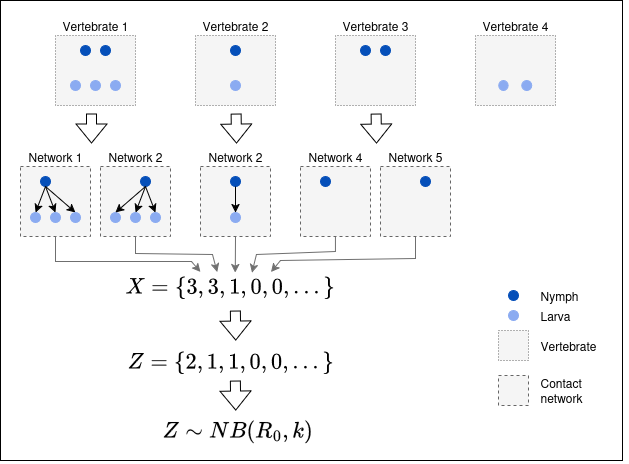
\includegraphics[width=1\textwidth, center]{coaggregation_data_diagram_mk3.drawio.png}
	\caption{A toy example of how we find the parameters for the offspring distribution. Each nymph has its own contact network with larvae. The out degree for each nymph is the number of larvae that it co-feeds with. A stochastic step is applied to the vector $ X $ to determine the number of larvae that become infectious nymphs, which is a vector $ Z $. $ R_0 $ and $ k $ are then found by fitting the reparameterised negative binomial distribution to $ Z $ as the offspring distribution.}
	\label{fig:coaggregation_diagram}
	\end{mdframed}
\end{figure}

This section has talked about using the negative binomial distribution for the offspring distribution. Several discrete distributions could be the best choice: geometric, Poisson and negative binomial distributions could all fit. The negative binomial distribution is often a good fit to parasite aggregation data, and, Lloyd-Smith et al showed this was the best fit for several disease transmission networks; we can expect that the negative binomial distribution will be the best fit. Later, we test the negative binomial distribution's goodness-of-fit against the Poisson and geometric distributions.

\subsection{Avoiding simulation of the offspring distribution to find \texorpdfstring{$ R_0 $}{R0}}

Conceptually, to find an offspring distribution we could i) fit a discrete distribution to $ X $ ii) draw random values from $ X $, iii) for each value drawn, apply a Bernoulli trial of $ \alpha $ to find $ Z $, iv) fit a distribution to $ Z $ to determine $ R_0 $ and $ k $. This sections shows that $ k $ can be found without the stochastic step to generate $ Z $. 

Let:

\begin{description}[leftmargin=1cm, style=nextline]
	\item[$ m = \frac{1}{n} \sum_i^n L_i $] be the mean of $ X $.
	\item[$ X \sim \text{NB}(m, k) $] be the co-aggregation distribution, fit to $ X $. This is the reparameterised negative binomial distribution (\ref{NegBinomReparam}).
	$ X_i $ is the number of larvae that are found to co-feed with a nymph of index $ i $.
	\item[$ I_{i,j} \sim \text{Bern}(p=\alpha) $] be a Bernoulli trial, or, a coin flip for each nymph of index $ i $ and for each larvae that it co-aggregates with, indexed by $ j \in 1:X_i $. This is a step where an infectious nymph generates a new infectious nymph in a branching process.
	\item[$ R_0 $] be the basic reproductive number. This is also the mean value of the offspring data $ Z $.
	\item[$ Z \sim \text{NB}(R_0, k) $] be the offspring distribution. This can be achieved by  simulating offspring data $ Z $ using $ X, \alpha $ and then fitting the distribution to it.
\end{description}

To get the expected number of new infectious nymphs per current infectious nymph, dependent on the number of larvae that each infectious nymph co-feeds with, the number of new infections is a series of Bernoulli trials, where $ X_i $ is the number of trials. This is otherwise known as a binomial experiment:

\begin{align}
    I_i &= \sum_j^{X_i} I_{i,j} \nonumber \\
    I_i &\sim \text{Binom}(X_i,\alpha)\label{BinomialExperiment}
\end{align}

The expected value of the binomial distribution in \eqref{BinomialExperiment} is $ \mu_i = X_i \alpha $, which is the expected number of new infections for the nymph of index $ i $.

Then to determine $ R_0 $, which is the expected number of new infections in an offspring distribution, this is:

\begin{align}
    R_0 &= \frac{1}{n} \sum_i^n \mu_i \nonumber \\
    R_0 &= \frac{1}{n} \sum_i^n L_i \alpha \nonumber \\
    R_0 &= \alpha \frac{1}{n} \sum_i^n L_i \nonumber \\
    R_0 &= \alpha m \label{FindingR0FromCoaggregationMean}
\end{align}

Since the reparameterised negative binomial distribution has parameters with asymptotically orthogonal limits, then $ k $ will not vary between the distributions fitted to $ X $ and $ Z $. This implies that we can obtain the parameters of $ Z $, $ R_0 $ and $ k $, directly from the distribution fitted to $ X $.

\subsection{Goodness of fit tests for distributions fit to co-aggregation data \texorpdfstring{$ X $}{X}} 

Before using the reparameterised negative binomial distribution (\ref{NegBinomReparam}) for determining the probability of extinction with a single-type GWBP, we can check which distribution fits the co-aggregation data $ X $ best. Candidate distributions are the negative binomial, Poisson and geometric distributions. We compared the fitted distributions visually, and then by using the Akaike Information Criterion (AIC) \cite{LloydSmith2005}.

For the visual analysis of each subset of Kielder Forest data, we calculated the error of each fitted distribution by finding the difference between its cumulative density function (CDF) and the data's empirical cumulative density function (eCDF) for the independent variable $ x $ of each function. These are presented in the results section, in Figures: \ref{fig:CDF_2004_iricinus_SA}, \ref{fig:CDF_2004_itrianguliceps_SA}, \ref{fig:CDF_2005_iricnus_FV}, \ref{fig:CDF_2005_itrianguliceps_FV}, \ref{fig:CDF_2005_itrianguliceps_SA}.

\begin{figure}[]
	\begin{mdframed}[backgroundcolor=grey250,rightline=false,leftline=false,topline=false]
	\centering
	\begin{tabular}{ll}
		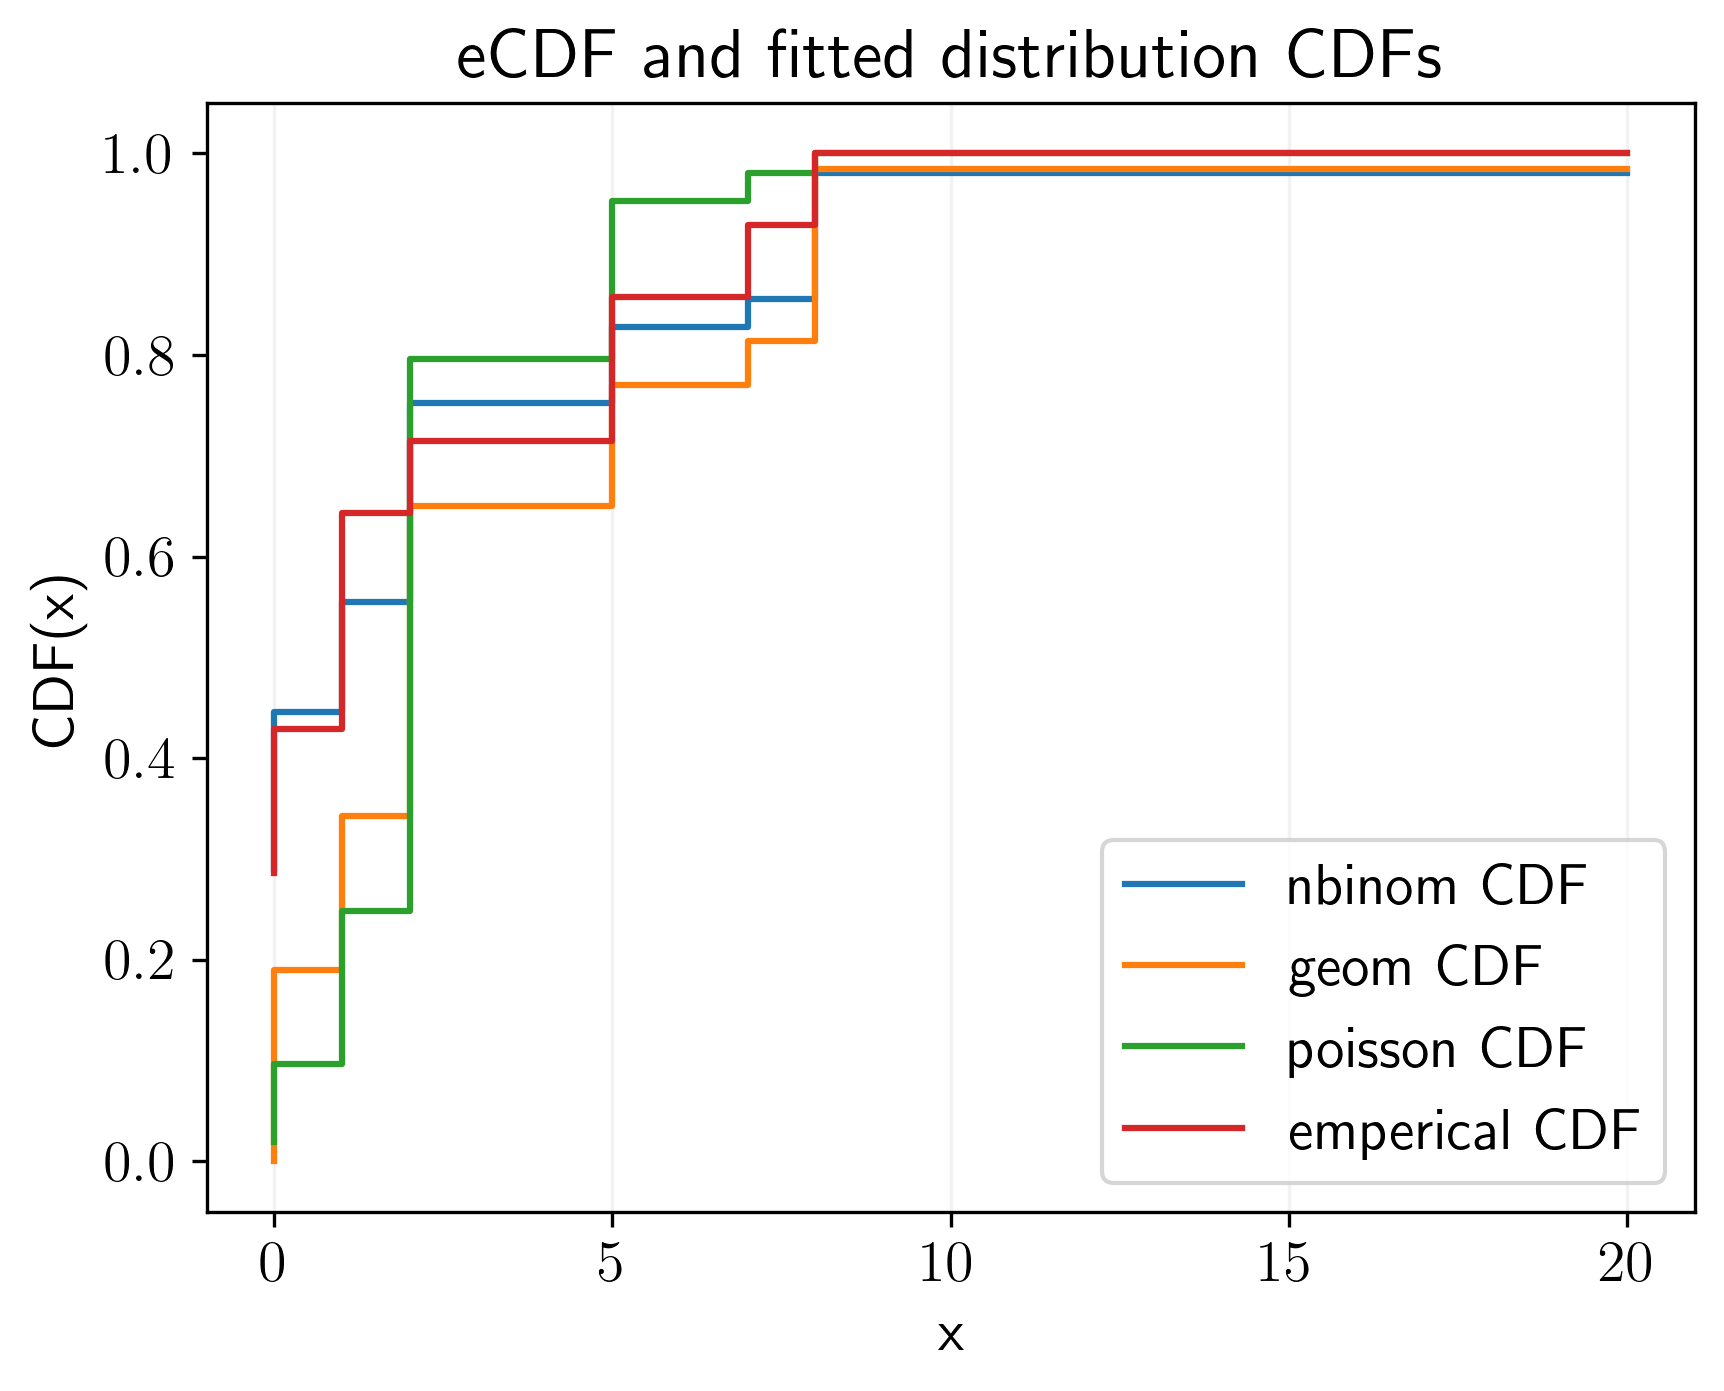
\includegraphics[width=.48\linewidth,valign=m]{CDF_compare_2004_I.ricinus_SA} & 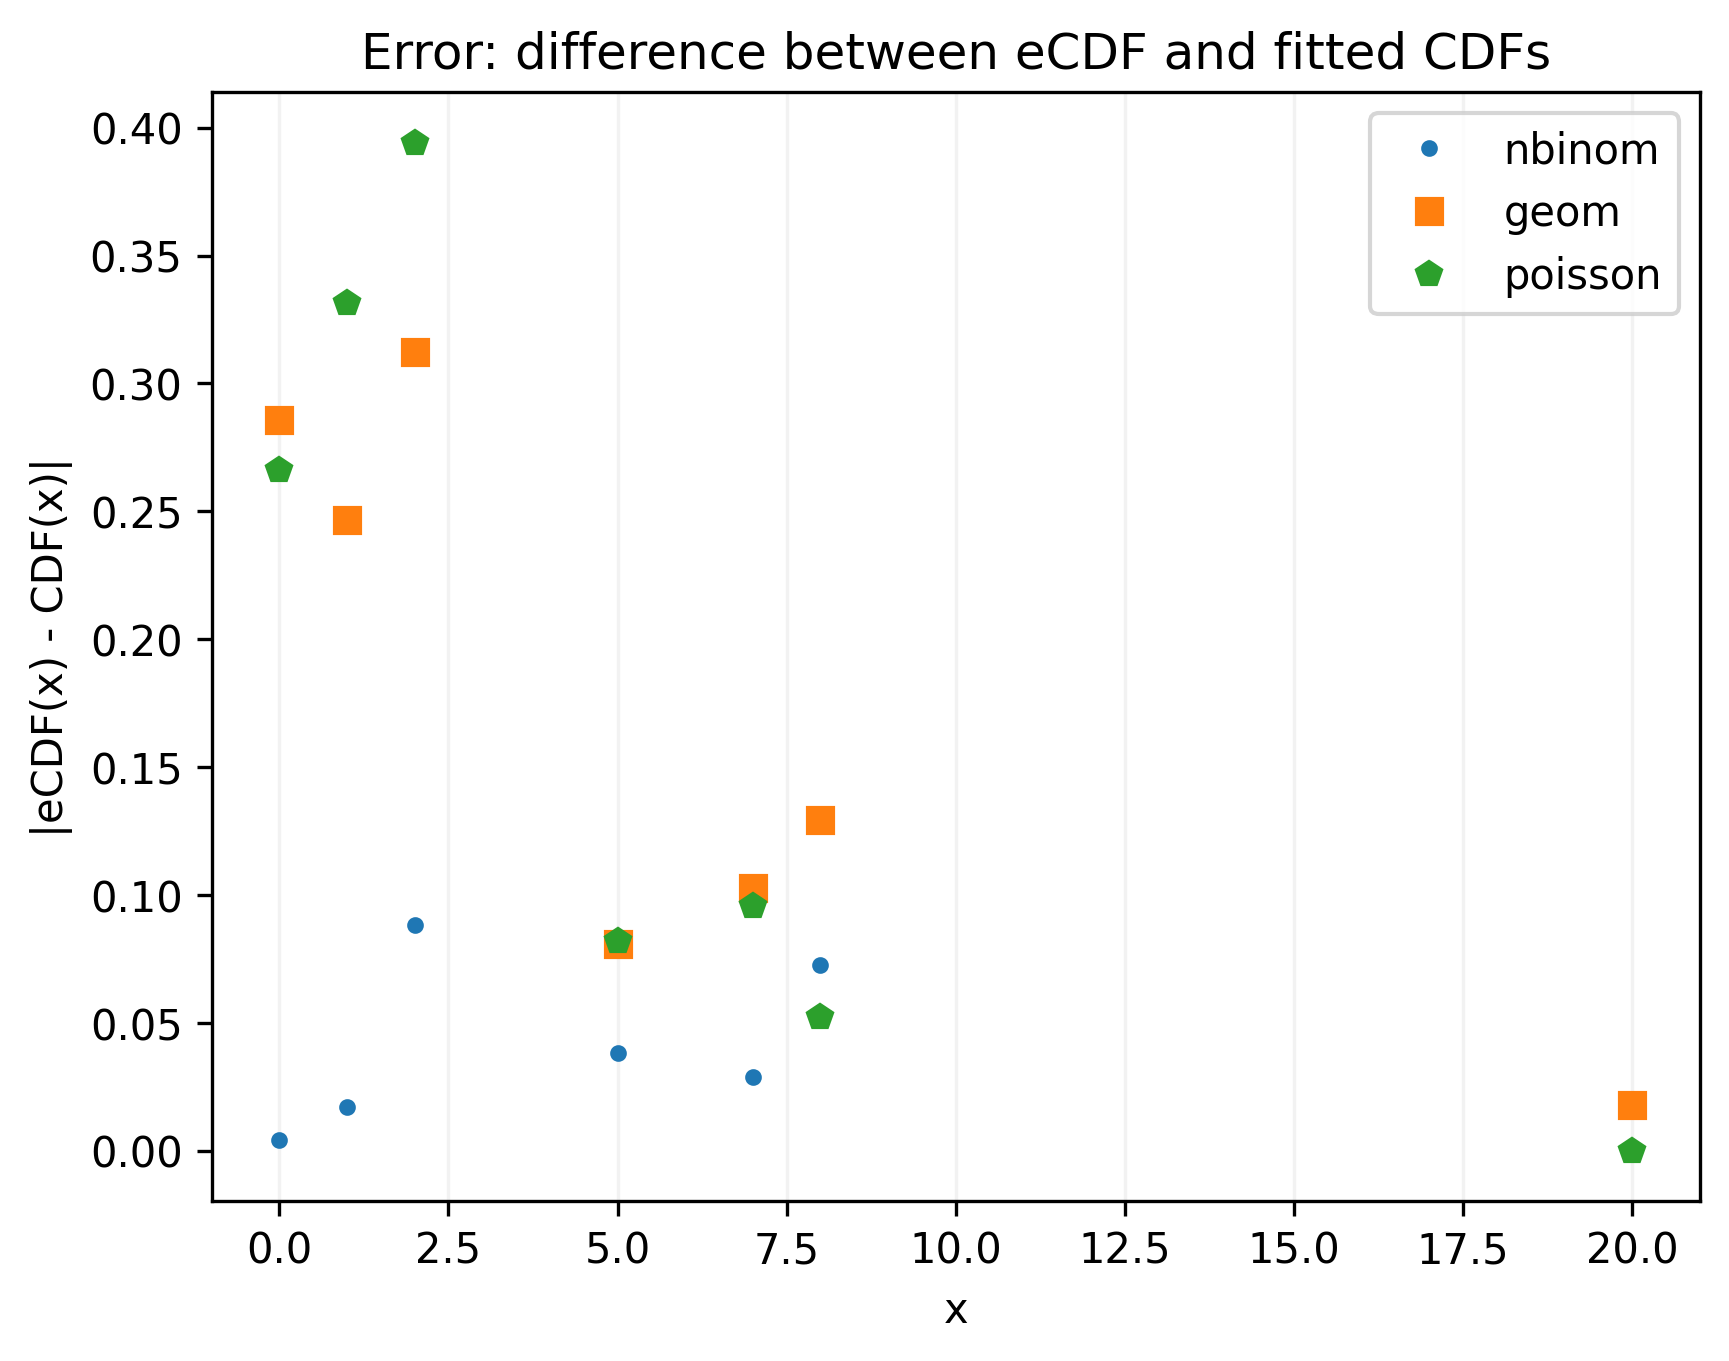
\includegraphics[width=.48\linewidth,valign=m]{CDF_errors_2004_I.ricinus_SA}
	\end{tabular}
	\caption{Discrete probability distributions fitted to the co-aggregation data $ X $ for \textit{I. ricinus} found on \textit{common shrews} in \textit{2004}.}
	\label{fig:CDF_2004_iricinus_SA}
	\end{mdframed}
\end{figure}

\begin{figure}[]
	\begin{mdframed}[backgroundcolor=grey250,rightline=false,leftline=false,topline=false]
	\centering
	\begin{tabular}{ll}
		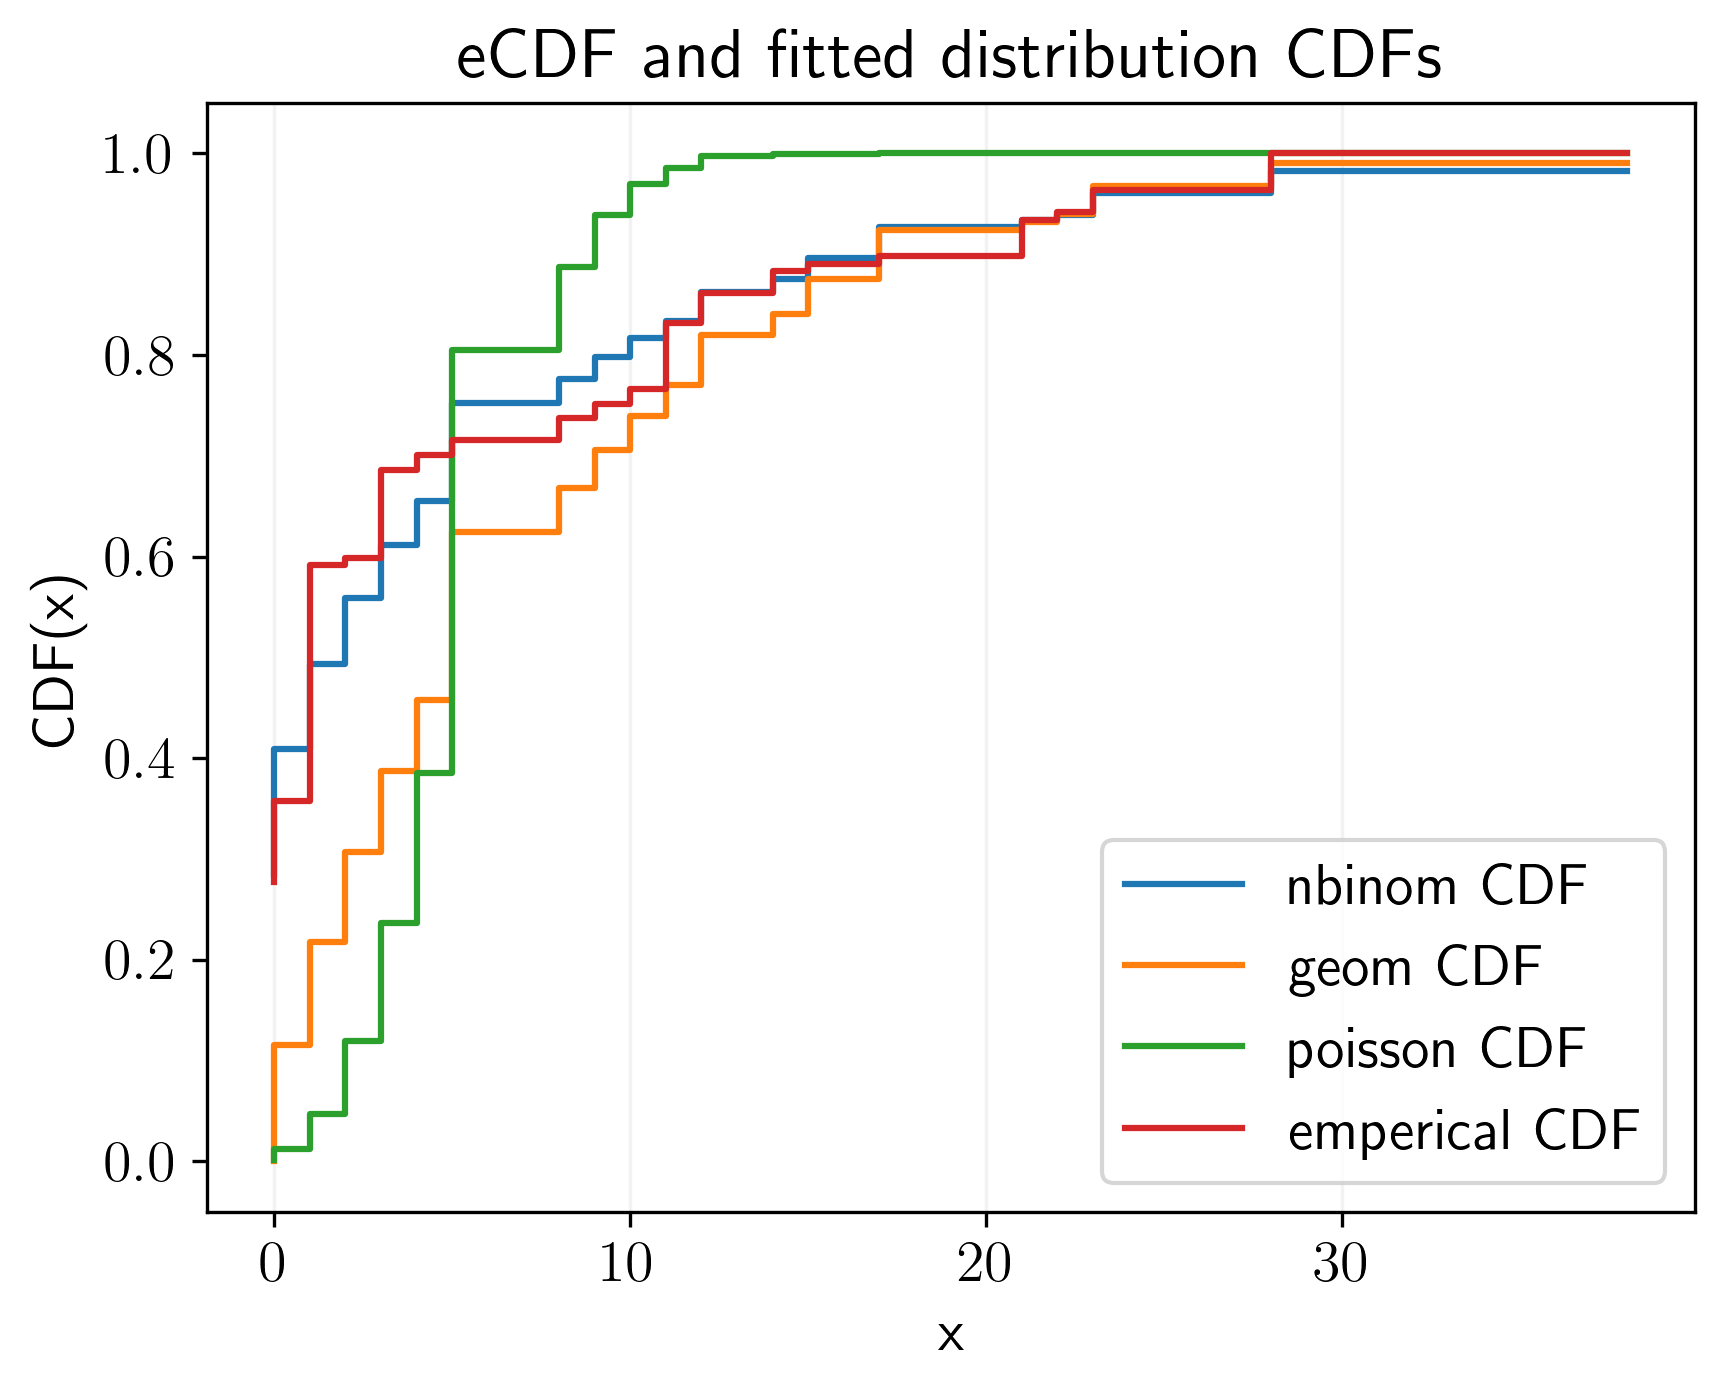
\includegraphics[width=.48\linewidth,valign=m]{CDF_compare_2004_I.trianguliceps_SA} & 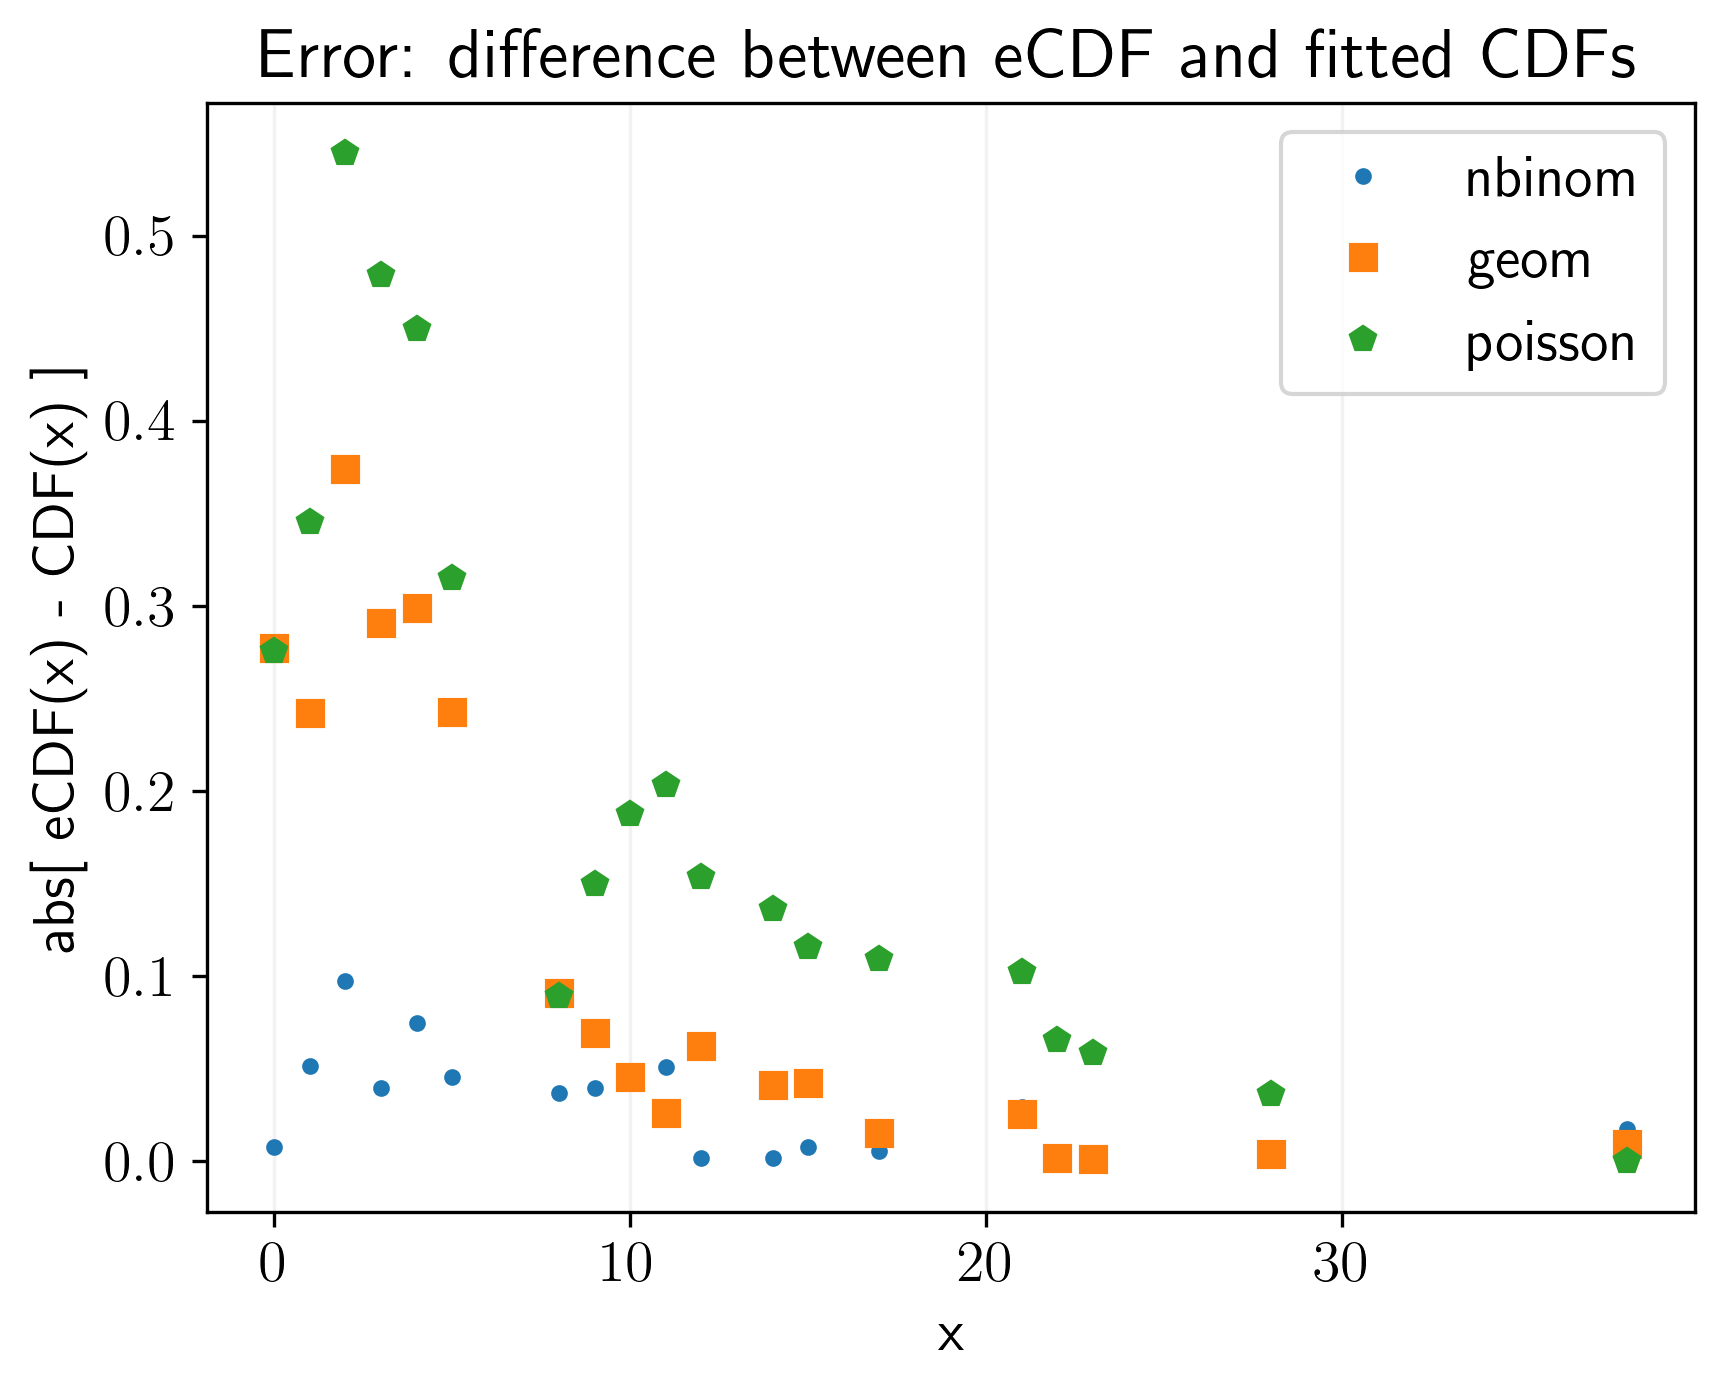
\includegraphics[width=.48\linewidth,valign=m]{CDF_errors_2004_I.trianguliceps_SA}
	\end{tabular}
	\caption{Discrete probability distributions fitted to the co-aggregation data $ X $ for \textit{I. trianguliceps} found on \textit{common shrews} in \textit{2004}.}
	\label{fig:CDF_2004_itrianguliceps_SA}
	\end{mdframed}
\end{figure}

\begin{figure}[]
	\begin{mdframed}[backgroundcolor=grey250,rightline=false,leftline=false,topline=false]
	\centering
	\begin{tabular}{ll}
		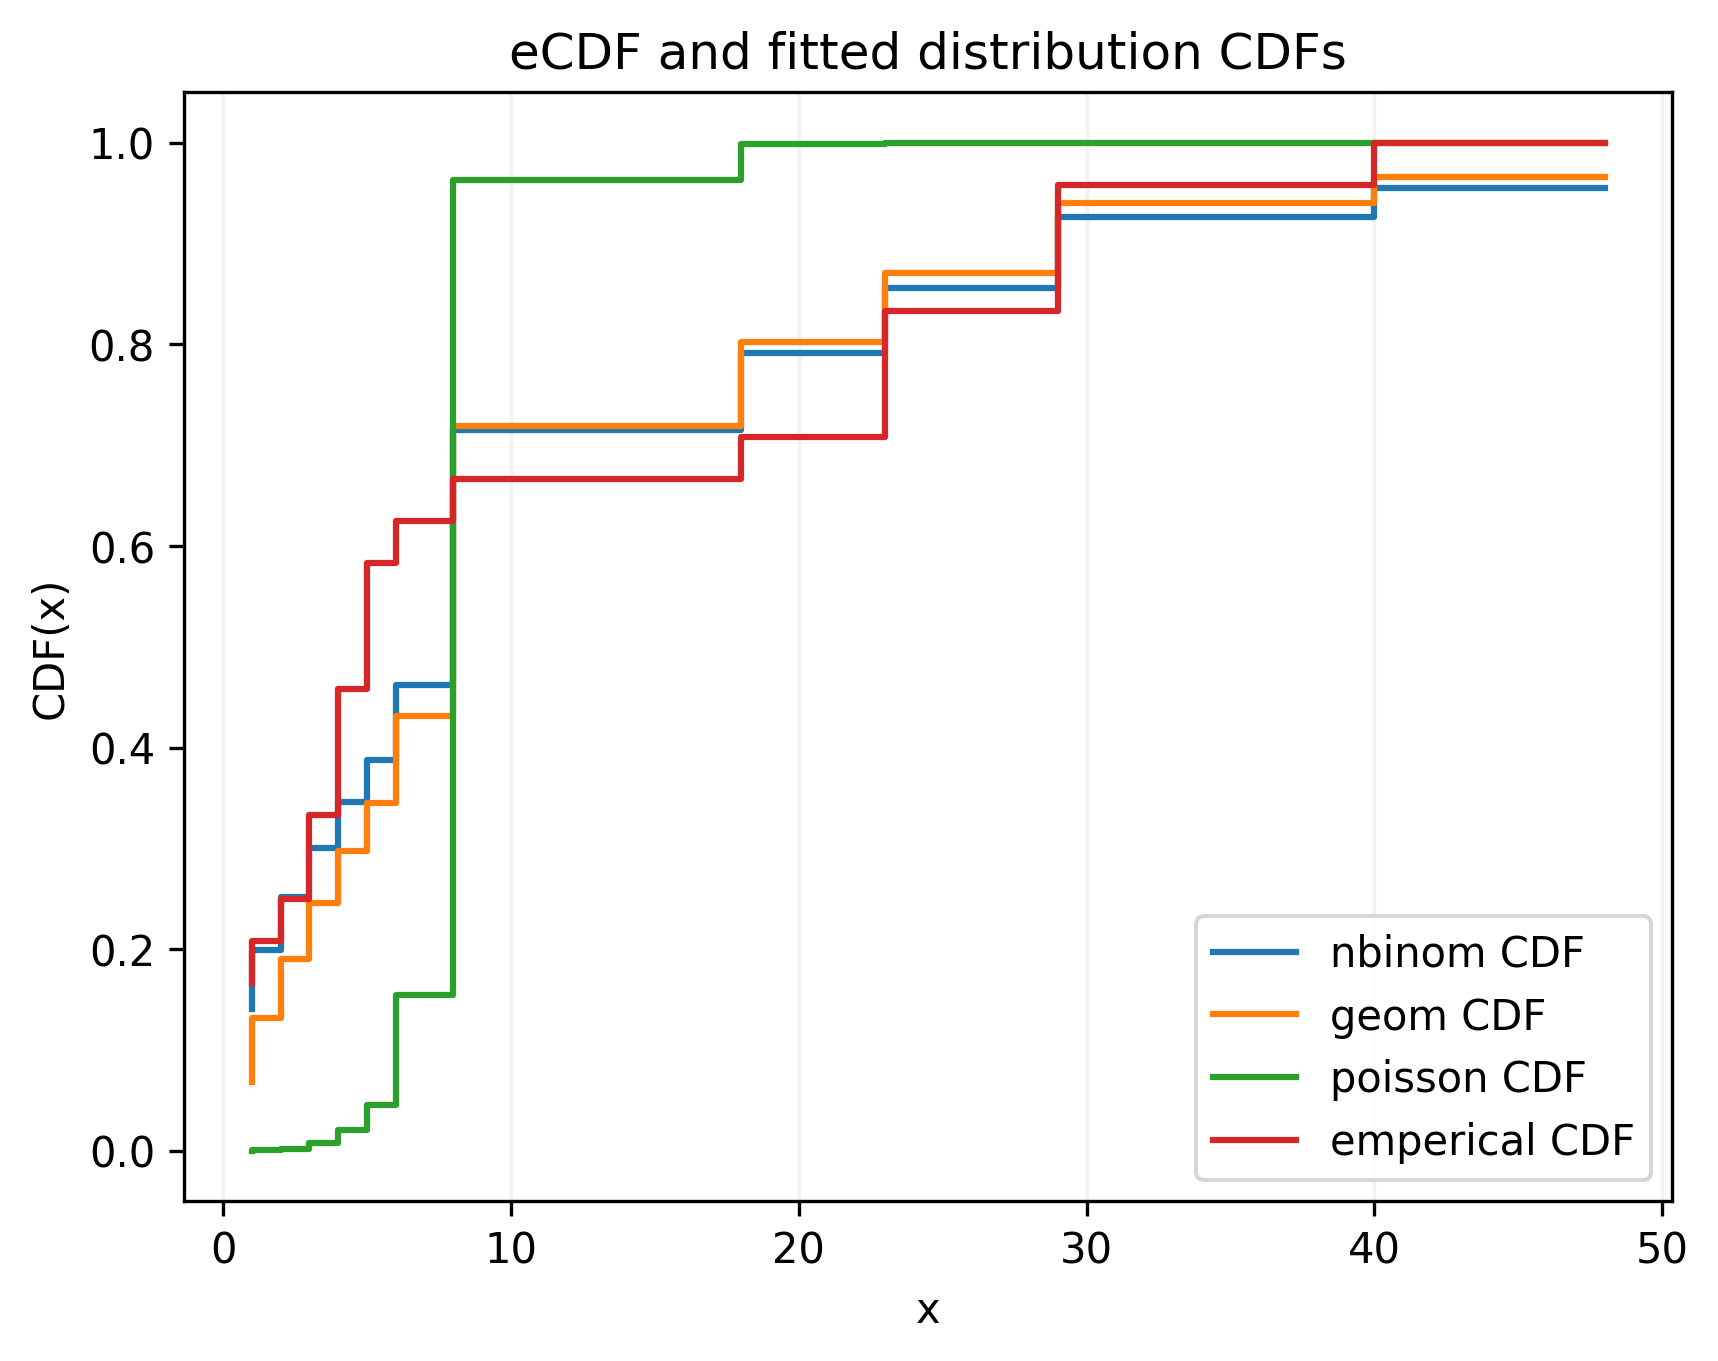
\includegraphics[width=.48\linewidth,valign=m]{CDF_compare_2005_I.ricinus_FV} & 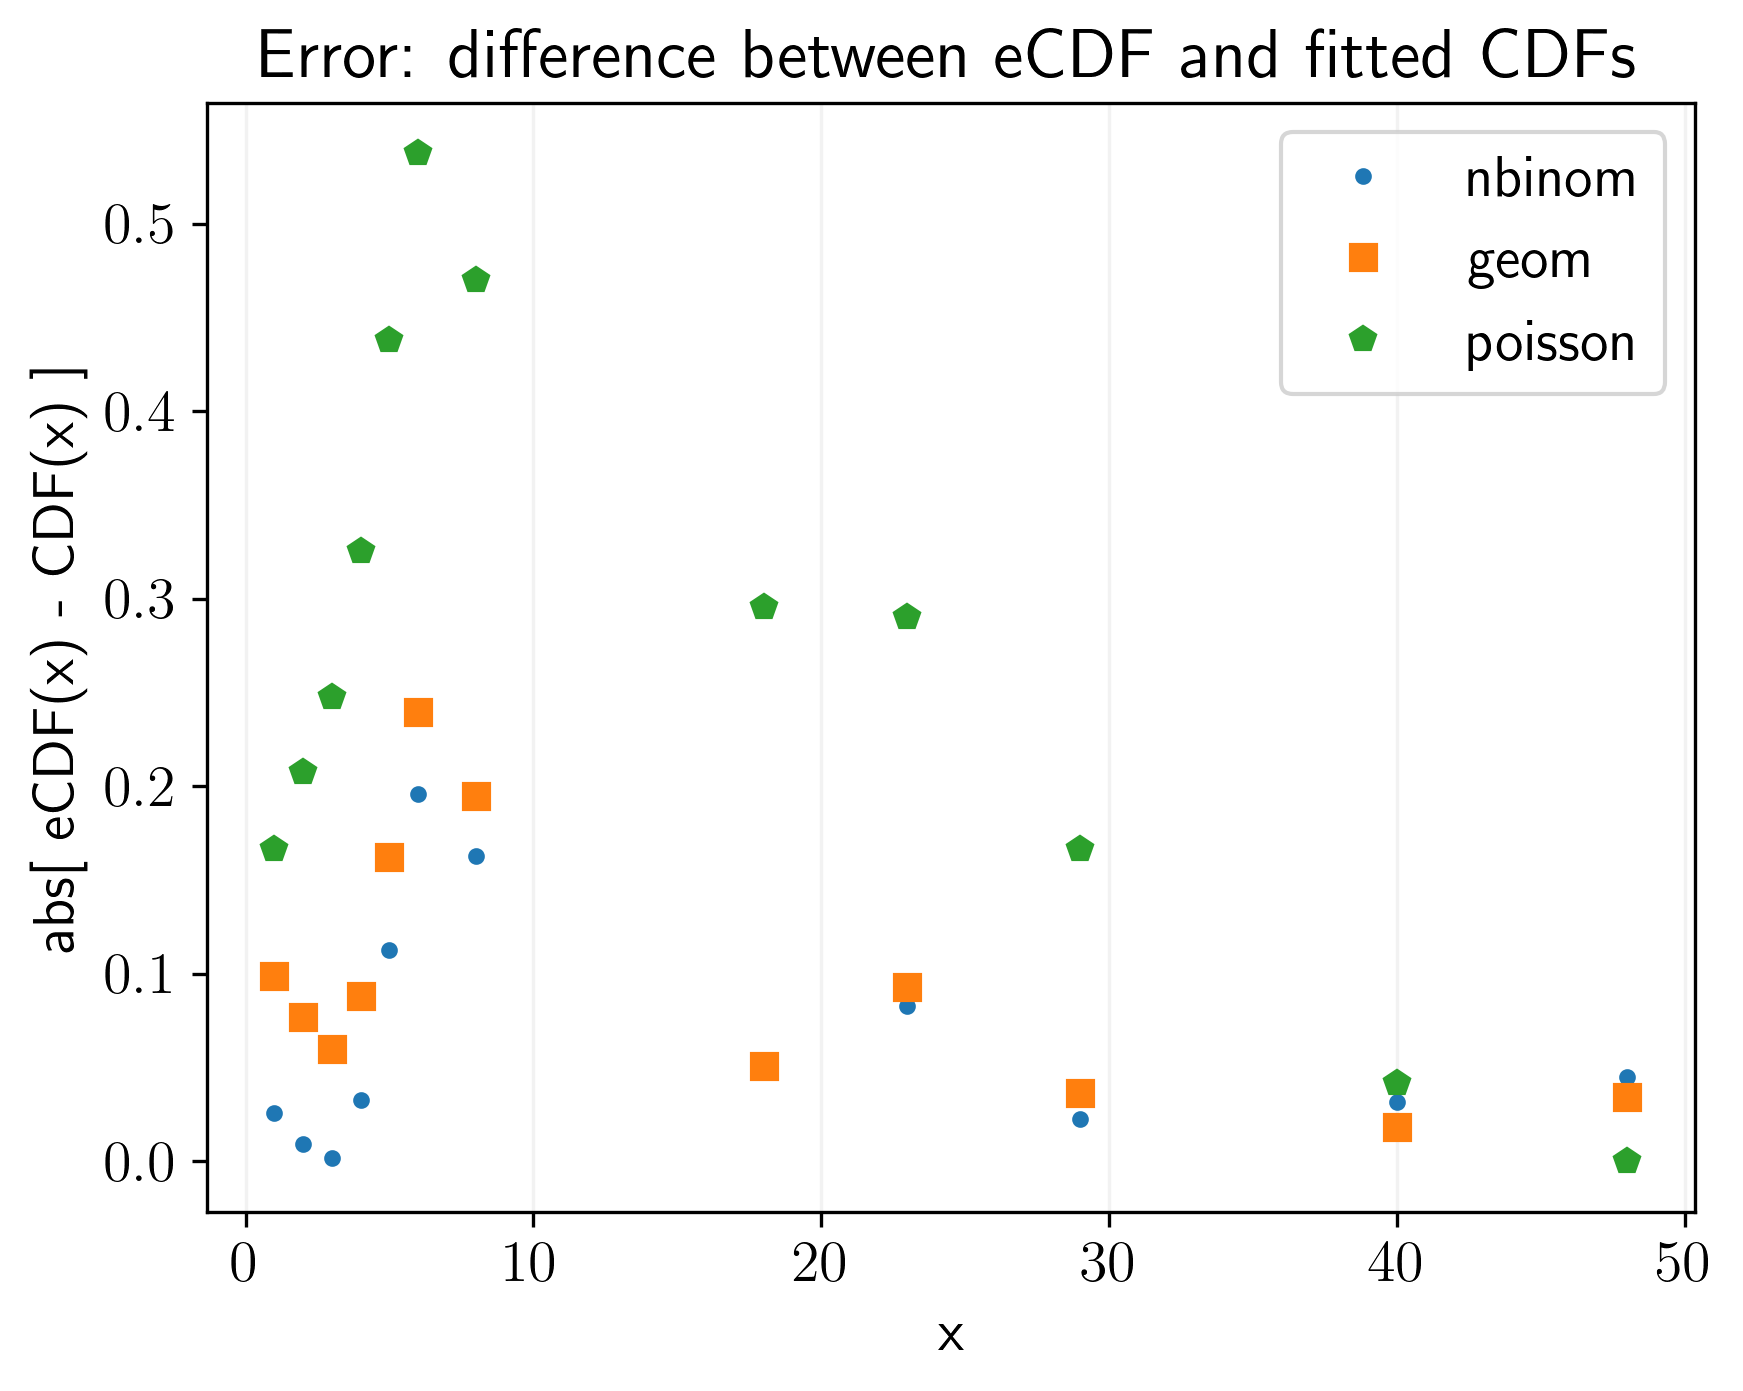
\includegraphics[width=.48\linewidth,valign=m]{CDF_errors_2005_I.ricinus_FV}
	\end{tabular}
	\caption{Discrete probability distributions fitted to the co-aggregation data $ X $ for \textit{I. ricinus} found on \textit{field voles} in \textit{2005}.}
	\label{fig:CDF_2005_iricnus_FV}
	\end{mdframed}
\end{figure}

\begin{figure}[]
	\begin{mdframed}[backgroundcolor=grey250,rightline=false,leftline=false,topline=false]
	\centering
	\begin{tabular}{ll}
	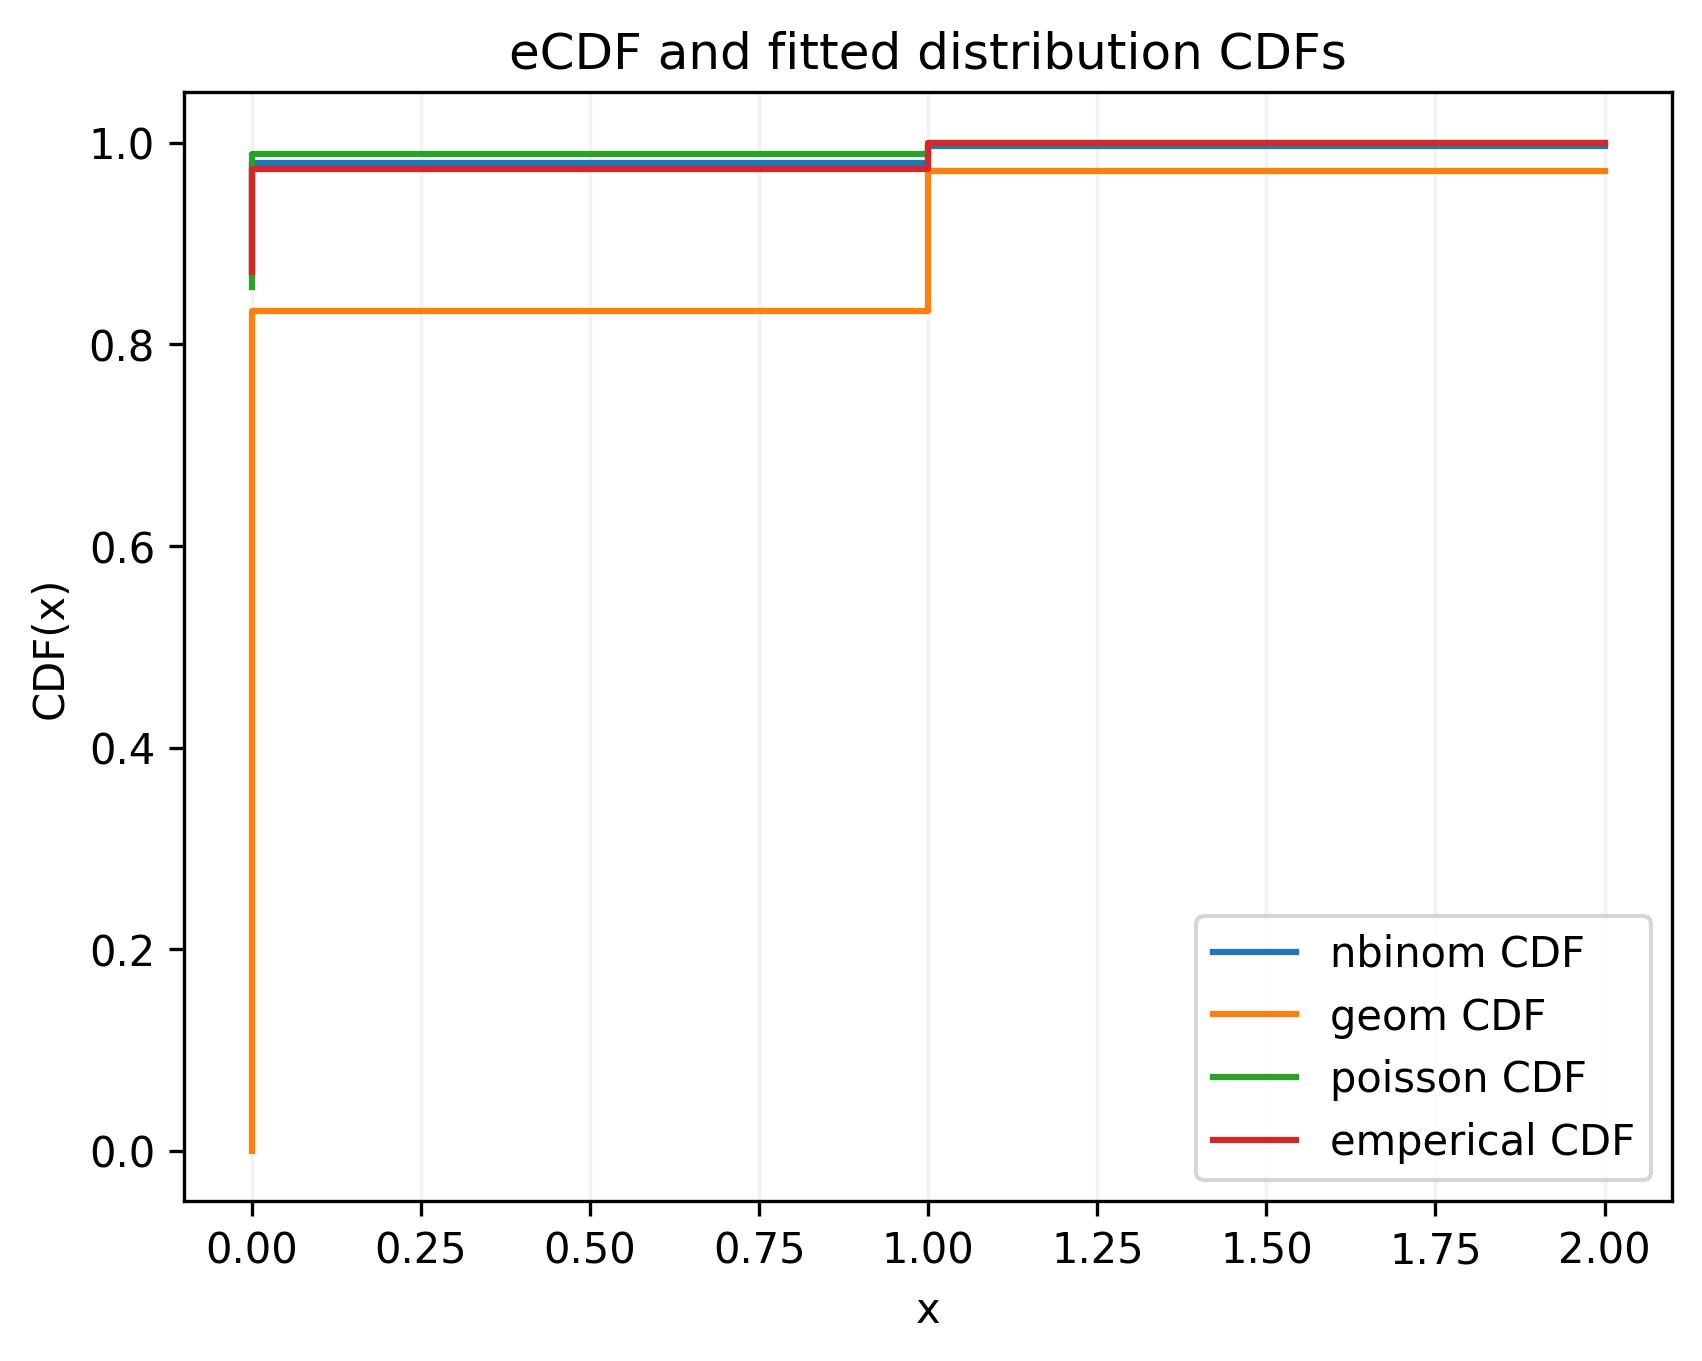
\includegraphics[width=.48\linewidth,valign=m]{CDF_compare_2005_I.trianguliceps_FV} & 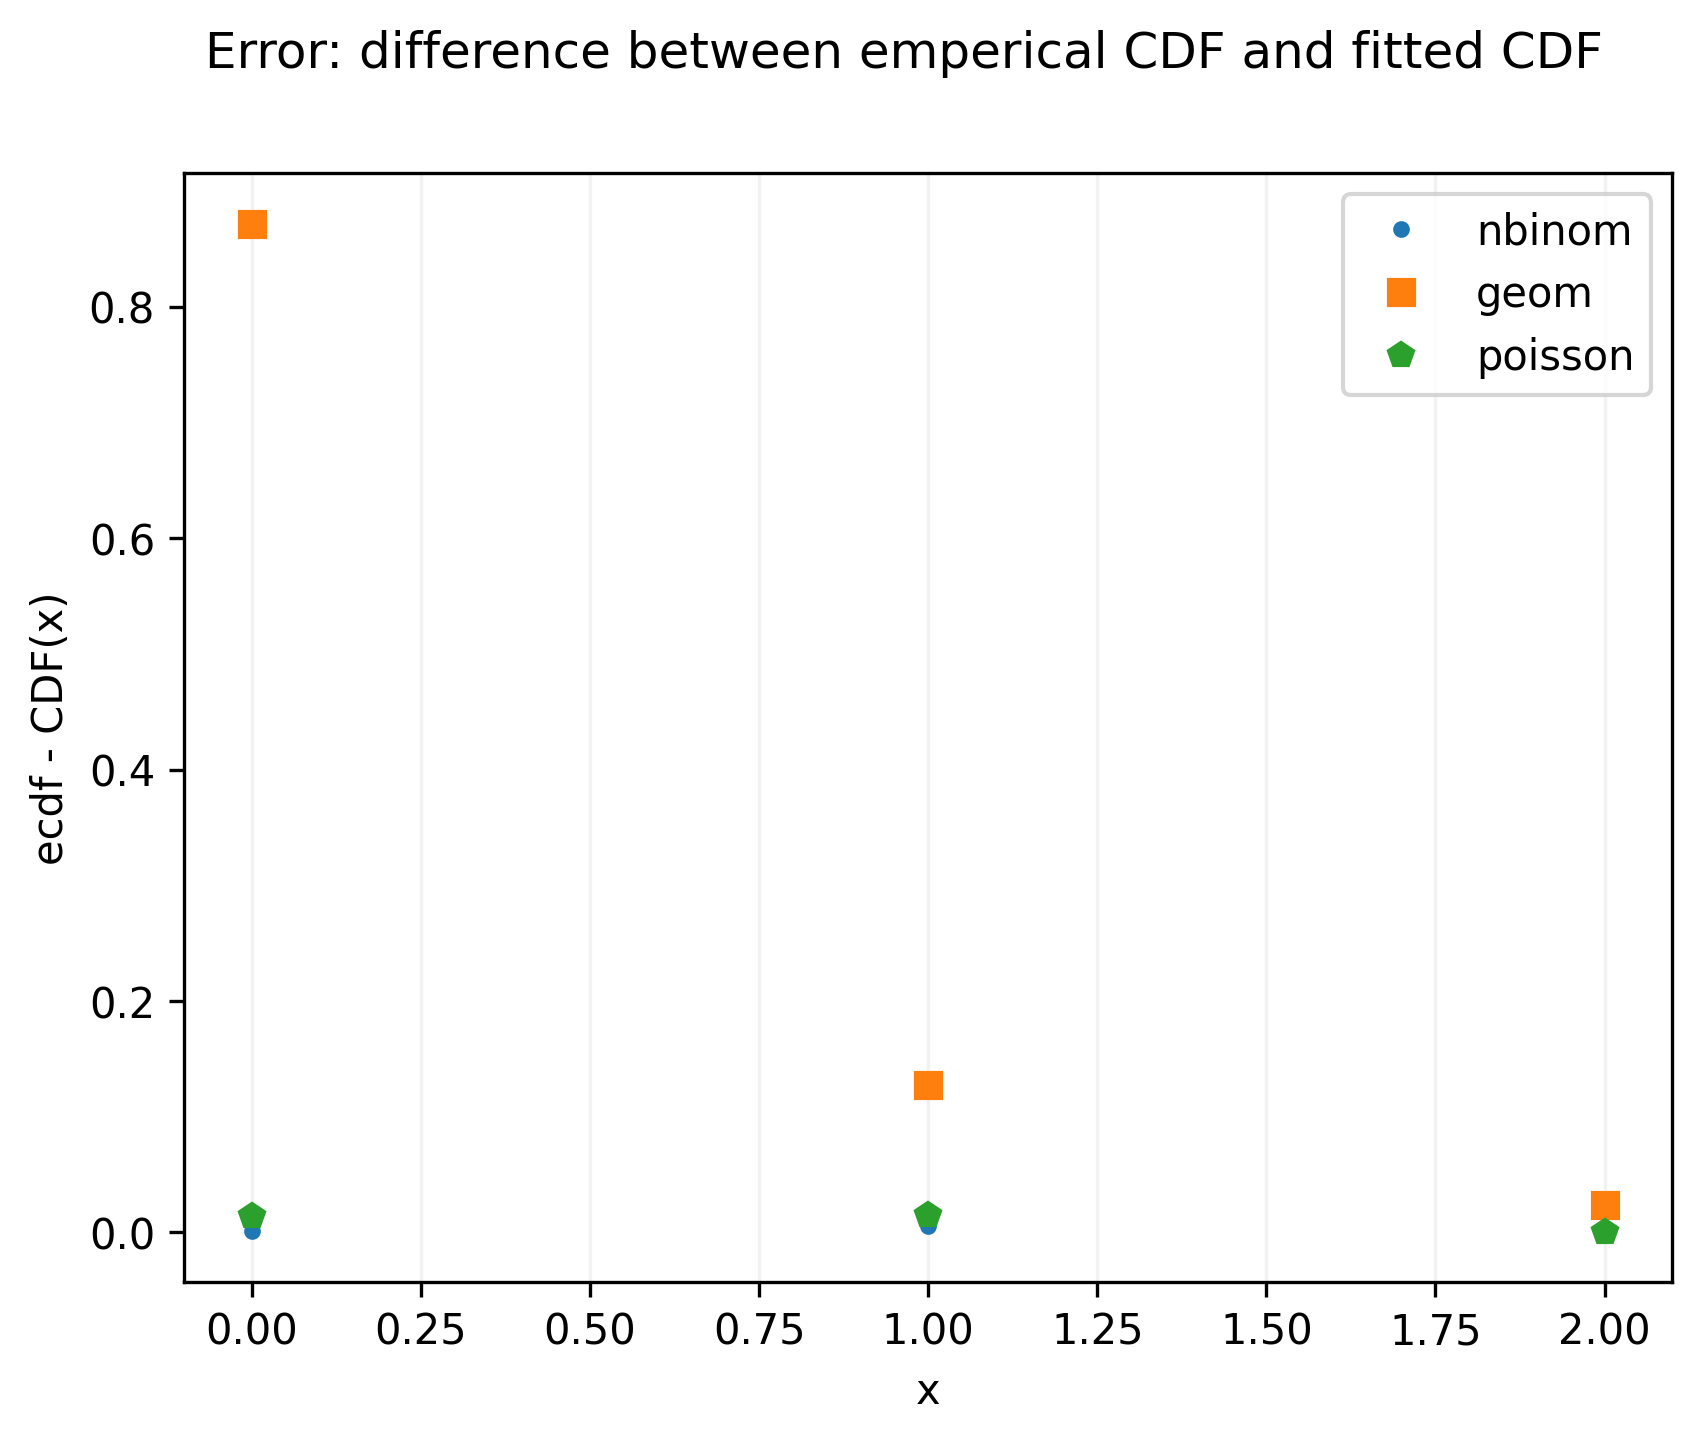
\includegraphics[width=.48\linewidth,valign=m]{CDF_errors_2005_I.trianguliceps_FV}
	\end{tabular}
		\caption{Discrete probability distributions fitted to the co-aggregation data $ X $ for \textit{I. trianguliceps} found on \textit{field voles} in \textit{2005}.}
	\label{fig:CDF_2005_itrianguliceps_FV}
	\end{mdframed}
\end{figure}

\begin{figure}[]
	\begin{mdframed}[backgroundcolor=grey250,rightline=false,leftline=false,topline=false]
	\centering
	\begin{tabular}{ll}
	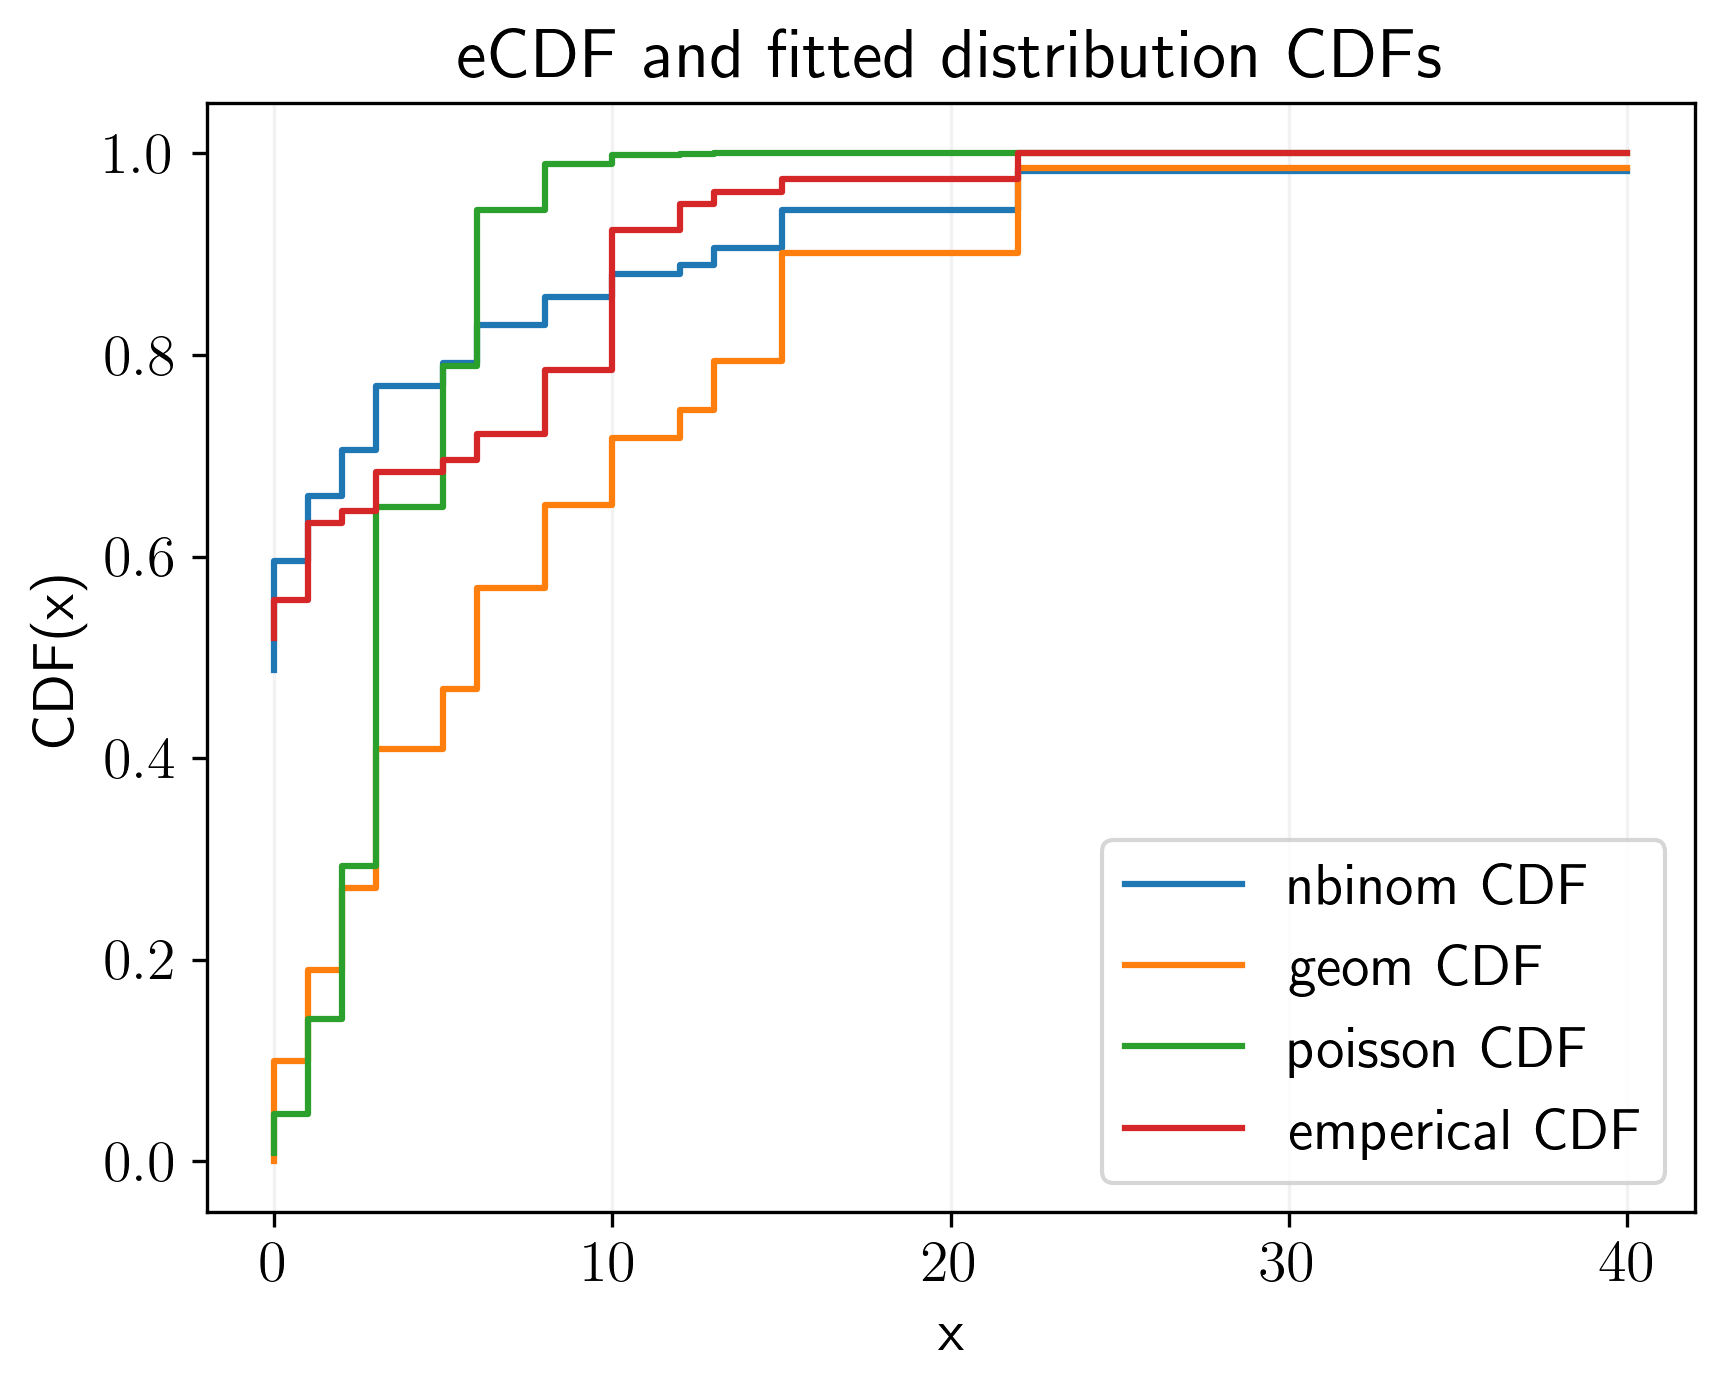
\includegraphics[width=.48\linewidth,valign=m]{CDF_compare_2005_I.trianguliceps_SA} & 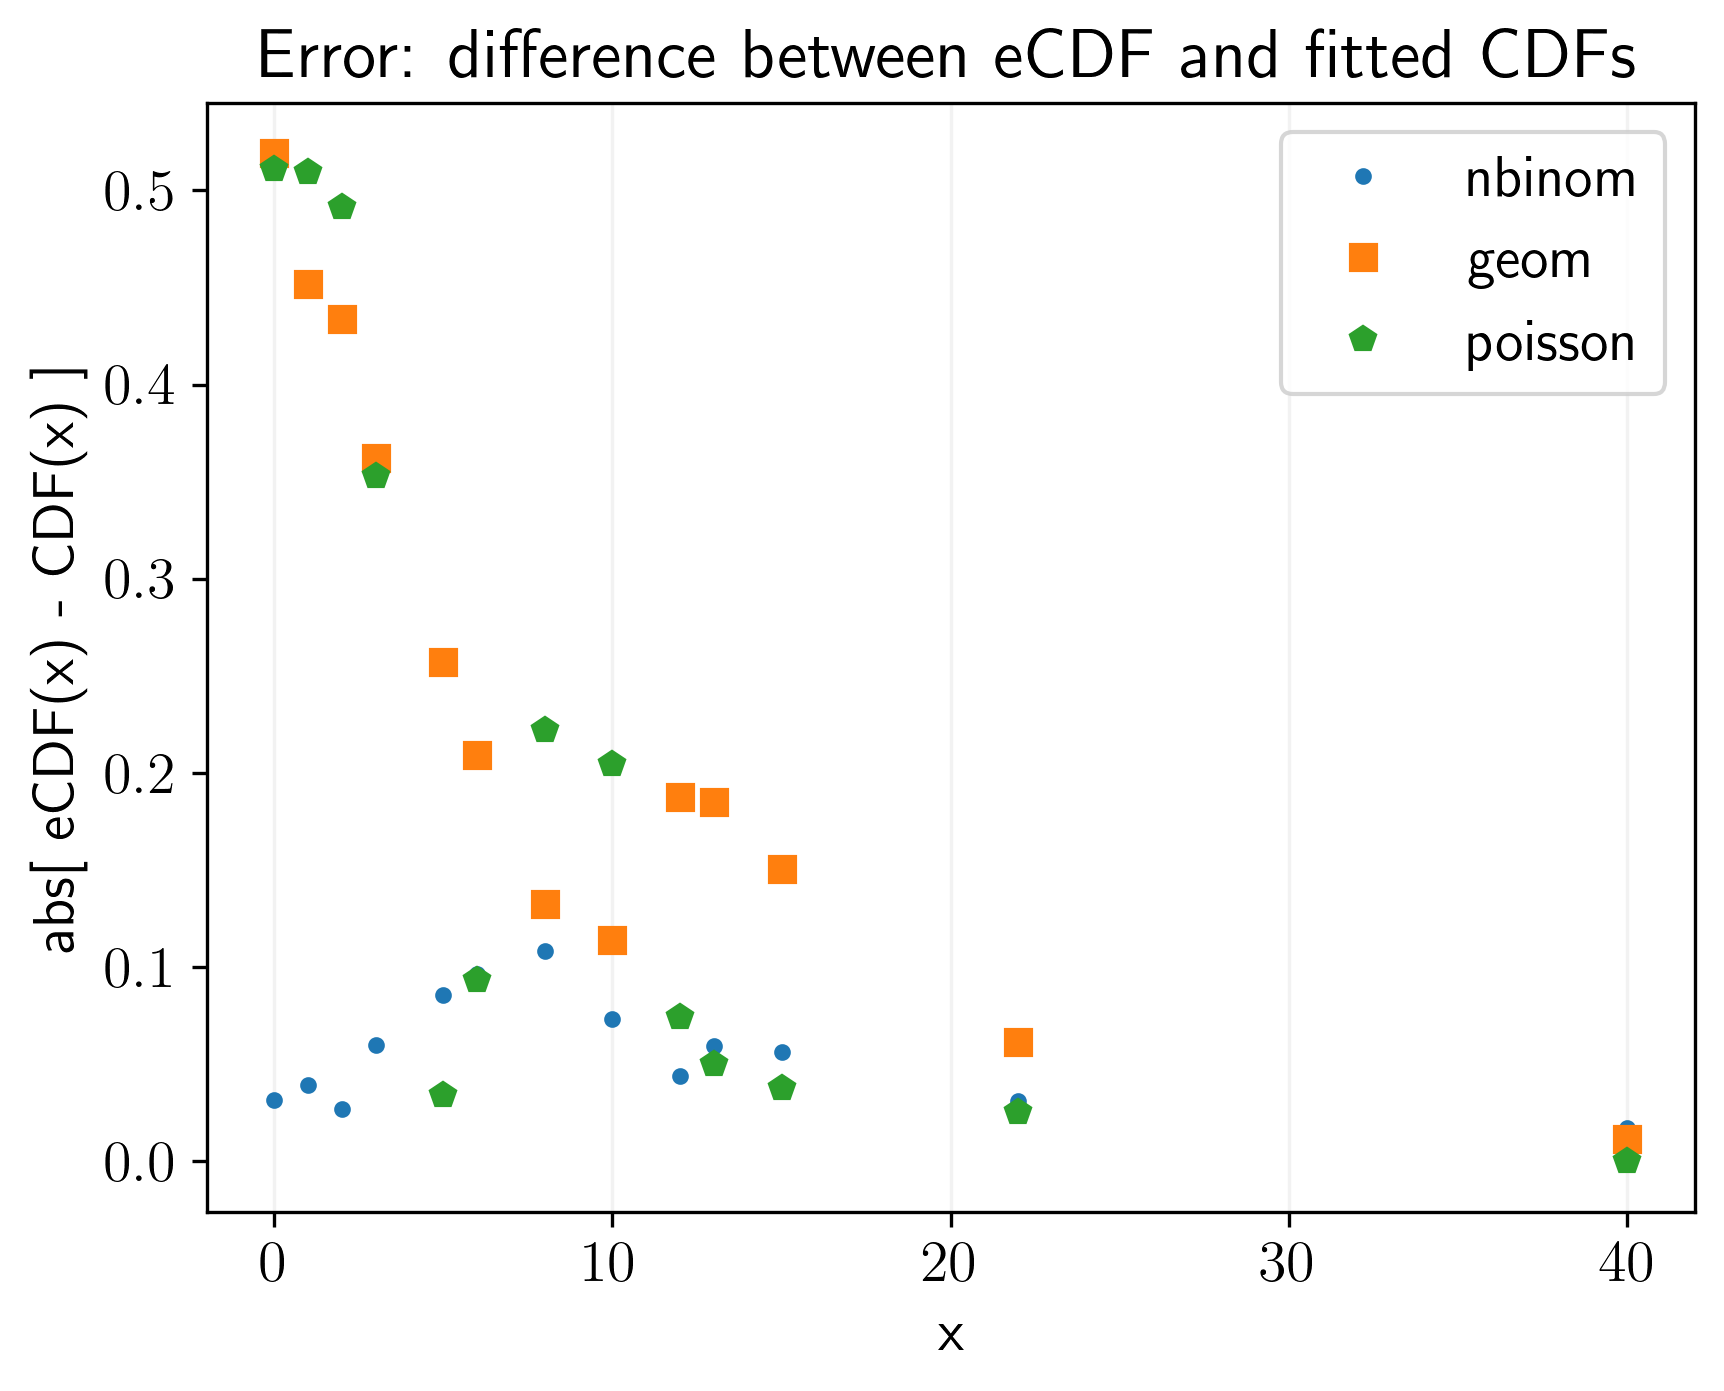
\includegraphics[width=.48\linewidth,valign=m]{CDF_errors_2005_I.trianguliceps_SA}
	\end{tabular}
		\caption{Discrete probability distributions fitted to the co-aggregation data $ X $ for \textit{I. trianguliceps} found on \textit{common shrews} in \textit{2005}.}
	\label{fig:CDF_2005_itrianguliceps_SA}
	\end{mdframed}
\end{figure}

To calculate goodness of fit, for each distribution and for each subset of data, we used $ AIC_c $ as did the Lloyd-Smith et al paper, which is $ AIC $ but corrected for small datasets. $ AIC_c $ rewards the best-fitting models while penalising models by their number of parameters. In the sense that the negative binomial, Poisson and geometric distributions are models, the negative binomial distribution will be penalised for its extra parameter, while the Poisson and geometric distributions will each be rewarded for having just one parameter. 

Each distributions' fit to co-aggregation data were calculated as:

\begin{align} \label{AIC}
    AIC &= 2K - 2\ln(L(\hat \theta | X)) \nonumber \\
    AIC_c &= AIC + \frac{2K(K+1)}{n-K-1}
\end{align}

For the Kielder Forest data, these $ AIC_c $ scores are presented in Table \ref{tab:kielderAIC}. A point of difference is that Lloyd-Smith and others scaled their $AIC_c $ by subtracting the smallest value in each dataset, but the smallest value in all tick burden datasets used in this project is always $ 0 $.

% Please add the following required packages to your document preamble:
% \usepackage{multirow}
\begin{table}[ht]
	\begin{mdframed}[backgroundcolor=grey250,rightline=false,leftline=false,topline=false]
	\centering
	\begin{tabular}{|l|l|l|rrr|}
		\hline
		\multirow{2}{*}{\textbf{Tick species}} & \multirow{2}{*}{\textbf{Host species}} & \multirow{2}{*}{\textbf{Year}} & \multicolumn{3}{c|}{\textbf{AICc}}                                                                                                \\ \cline{4-6} 
		&                                        &                                & \multicolumn{1}{c|}{\textbf{Negative binomial}} & \multicolumn{1}{c|}{\textbf{Geometric}} & \multicolumn{1}{c|}{\textbf{Poisson}} \\ \hline
		\textit{I. trianguliceps}              & \textit{Common shrew}                  & 2004                           & \multicolumn{1}{r|}{\textit{773.634}}           & \multicolumn{1}{r|}{$\infty$}           & 1811.540                              \\ \hline
		\textit{I. trianguliceps}              & \textit{Common shrew}                  & 2005                           & \multicolumn{1}{r|}{\textit{370.802}}           & \multicolumn{1}{r|}{$\infty$}           & 939.5                                 \\ \hline
		\textit{I. trianguliceps}              & \textit{Field vole}                    & 2005                           & \multicolumn{1}{r|}{74.768}                     & \multicolumn{1}{r|}{$\infty$}           & \textit{73.748}                       \\ \hline
		\textit{I. ricinus}                    & \textit{Common shrew}                  & 2004                           & \multicolumn{1}{r|}{\textit{73.725}}            & \multicolumn{1}{r|}{$\infty$}           & 115.538                               \\ \hline
		\textit{I. ricinus}                    & \textit{Field vole}                    & 2005                           & \multicolumn{1}{r|}{182.205}                    & \multicolumn{1}{r|}{\textit{176.696}}   & 471.78                                \\ \hline
	\end{tabular}
	\caption{AICc (corrected AIC), fitted to subsets of the Kielder Forest data. The negative binomial distribution is the best fit for 3 subsets of data, while it is nearly the best fit in 2 other cases.}
	\label{tab:kielderAIC}
	\end{mdframed}
\end{table}

\clearpage

\subsection{Results of fitting the negative binomial distribution to co-aggregation data \texorpdfstring{$ X $}{X}}

With the negative binomial distribution confirmed as the best (or close to the best) fit for the co-aggregation data, $ X $, we can now fit the reparameterised negative binomial distribution to subsets of the Kielder Forest data, to obtain the sample mean $ m $ and dispersion parameter $ k $.

Figures \ref{fig:distFit_2004_Iricinus_SA}, \ref{fig:distFit_2004_Itrianguliceps_SA}, \ref{fig:distFit_2005_Iricinus_FV}, \ref{fig:distFit_2005_Itrianguliceps_FV}, \ref{fig:distFit_2005_Itrianguliceps_SA}, show the results of MLE applied to the reparameterised negative binomial distribution for each of the 5 subsets of Kielder Forest data.

\begin{figure}[ht]
	\begin{mdframed}[backgroundcolor=grey250,rightline=false,leftline=false,topline=false]
	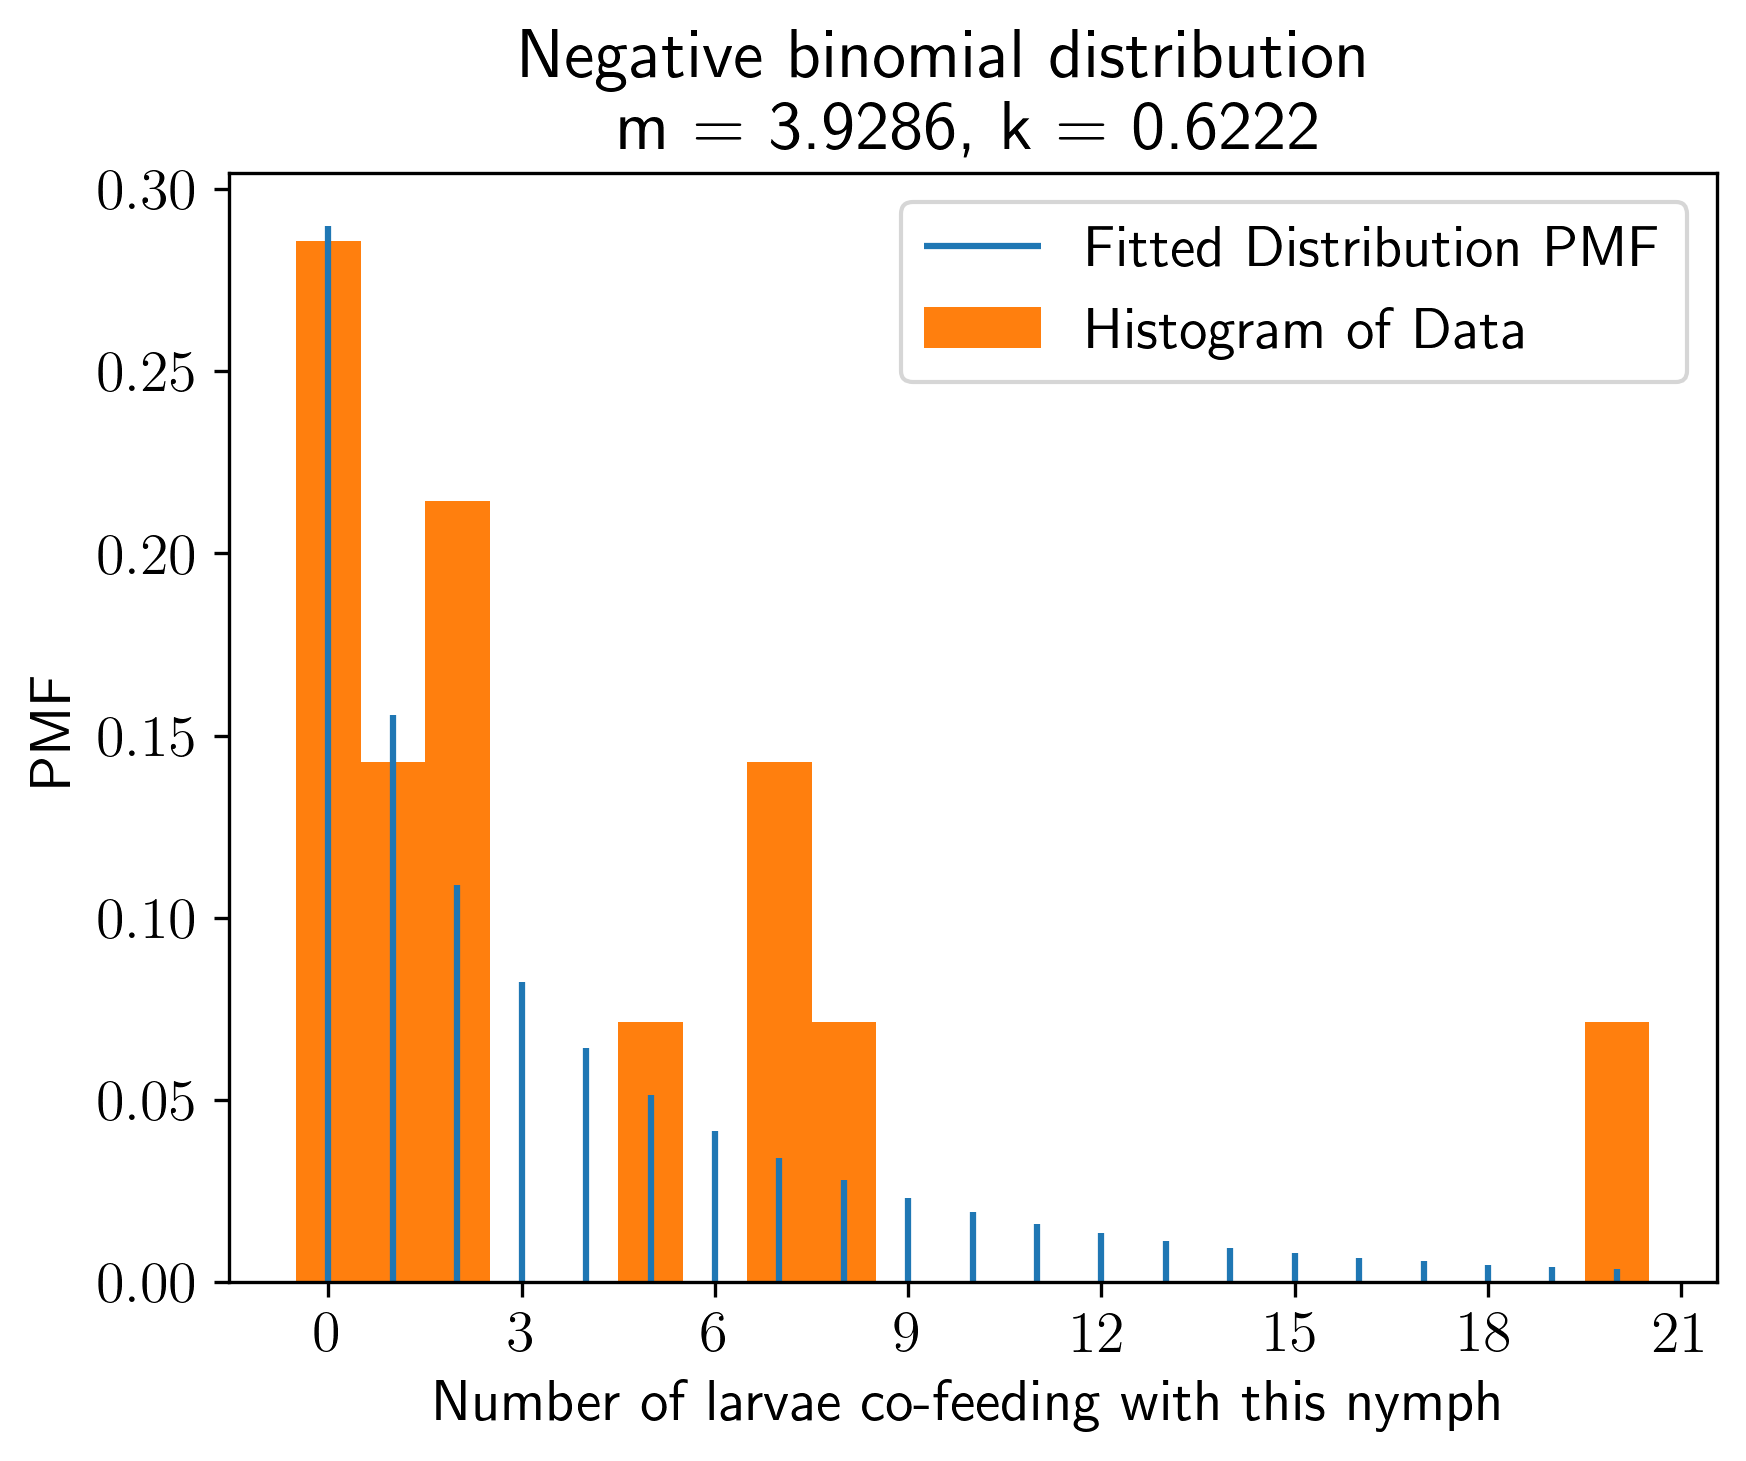
\includegraphics[width=0.5\textwidth, center]{coaggregation_dist_2004_I.ricinus_SA.png}
	\caption{For counts of \textit{I.ricinus} found on Common Shrews in 2004}\label{fig:distFit_2004_Iricinus_SA}
	\end{mdframed}
\end{figure}

\begin{figure}[ht]
	\begin{mdframed}[backgroundcolor=grey250,rightline=false,leftline=false,topline=false]
	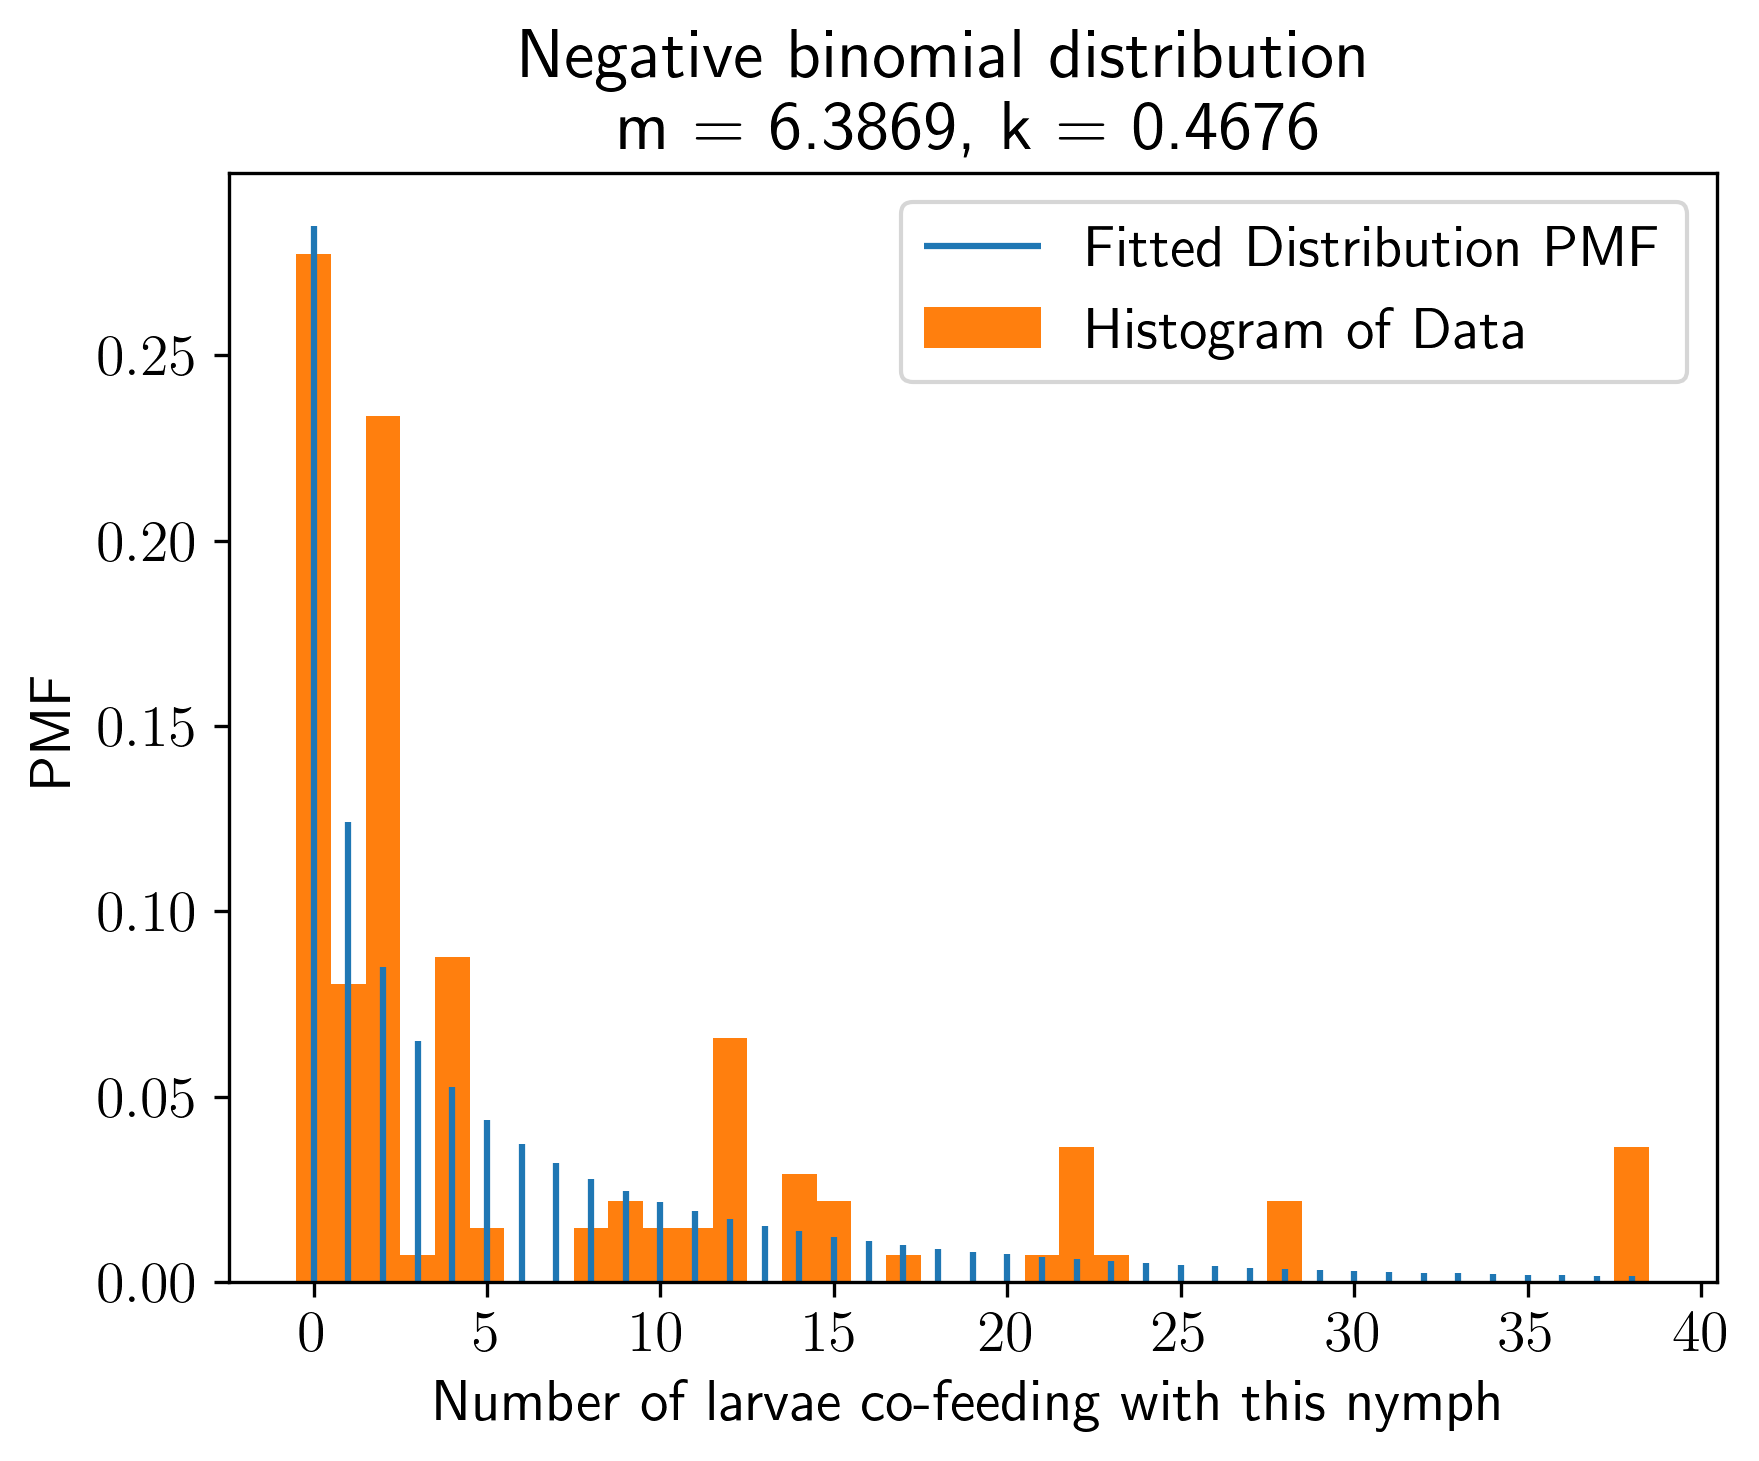
\includegraphics[width=0.5\textwidth, center]{coaggregation_dist_2004_I.trianguliceps_SA.png}
	\caption{For counts of \textit{I.trianguliceps} found on Common Shrews in 2004}\label{fig:distFit_2004_Itrianguliceps_SA}
	\end{mdframed}
\end{figure}

\begin{figure}[]
	\begin{mdframed}[backgroundcolor=grey250,rightline=false,leftline=false,topline=false]
	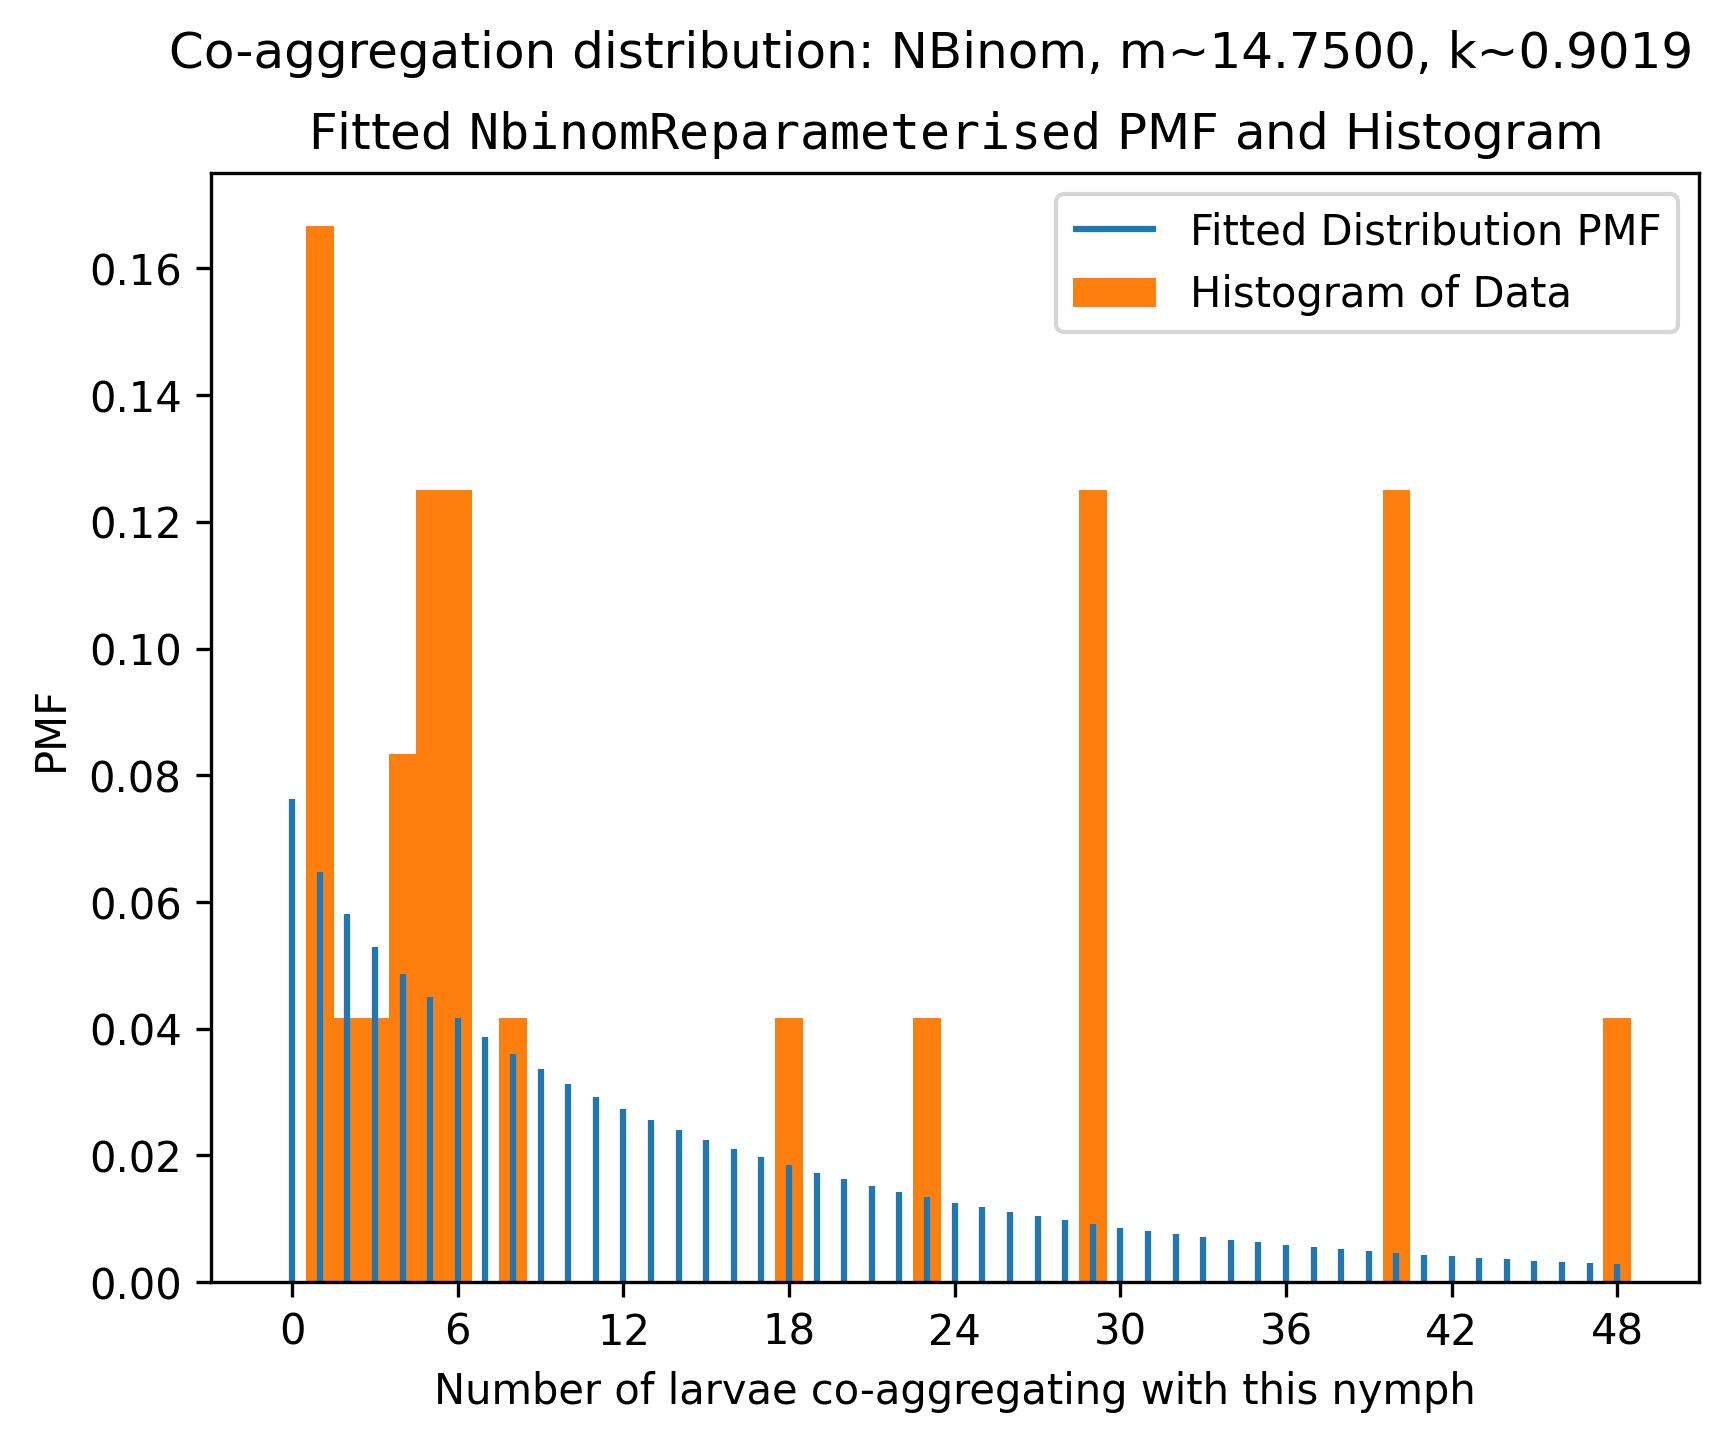
\includegraphics[width=0.5\textwidth, center]{coaggregation_dist_2005_I.ricinus_FV.png}
	\caption{For counts of \textit{I.ricinus} found on Field Voles in 2005}\label{fig:distFit_2005_Iricinus_FV}
	\end{mdframed}
\end{figure}

\begin{figure}[]
	\begin{mdframed}[backgroundcolor=grey250,rightline=false,leftline=false,topline=false]
	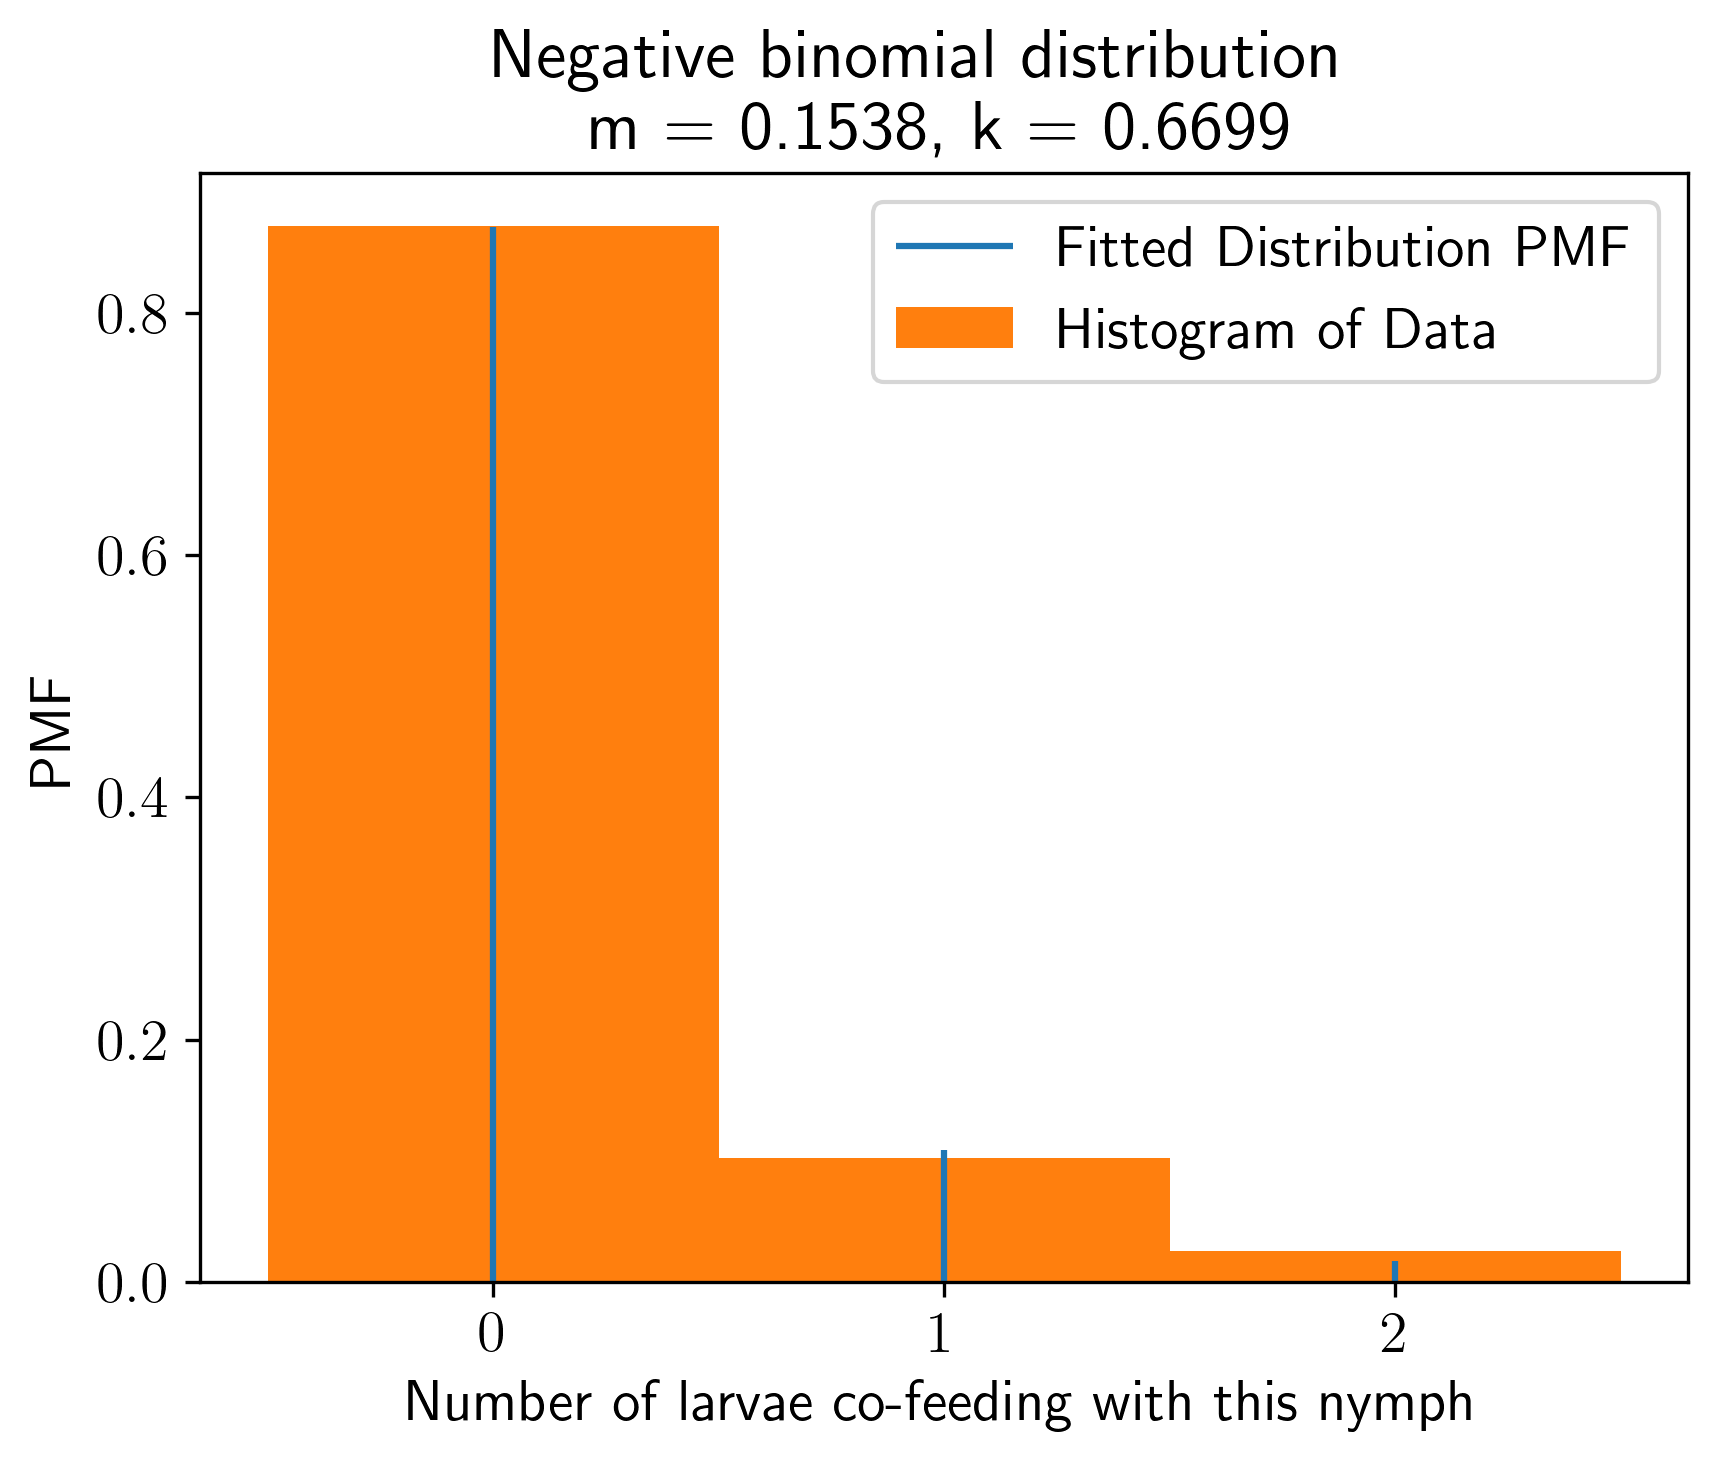
\includegraphics[width=0.5\textwidth, center]{coaggregation_dist_2005_I.trianguliceps_FV.png}
	\caption{For counts of \textit{I.trianguliceps} found on Field Voles in 2005}\label{fig:distFit_2005_Itrianguliceps_FV}
	\end{mdframed}
\end{figure}

\begin{figure}[]
	\begin{mdframed}[backgroundcolor=grey250,rightline=false,leftline=false,topline=false]
	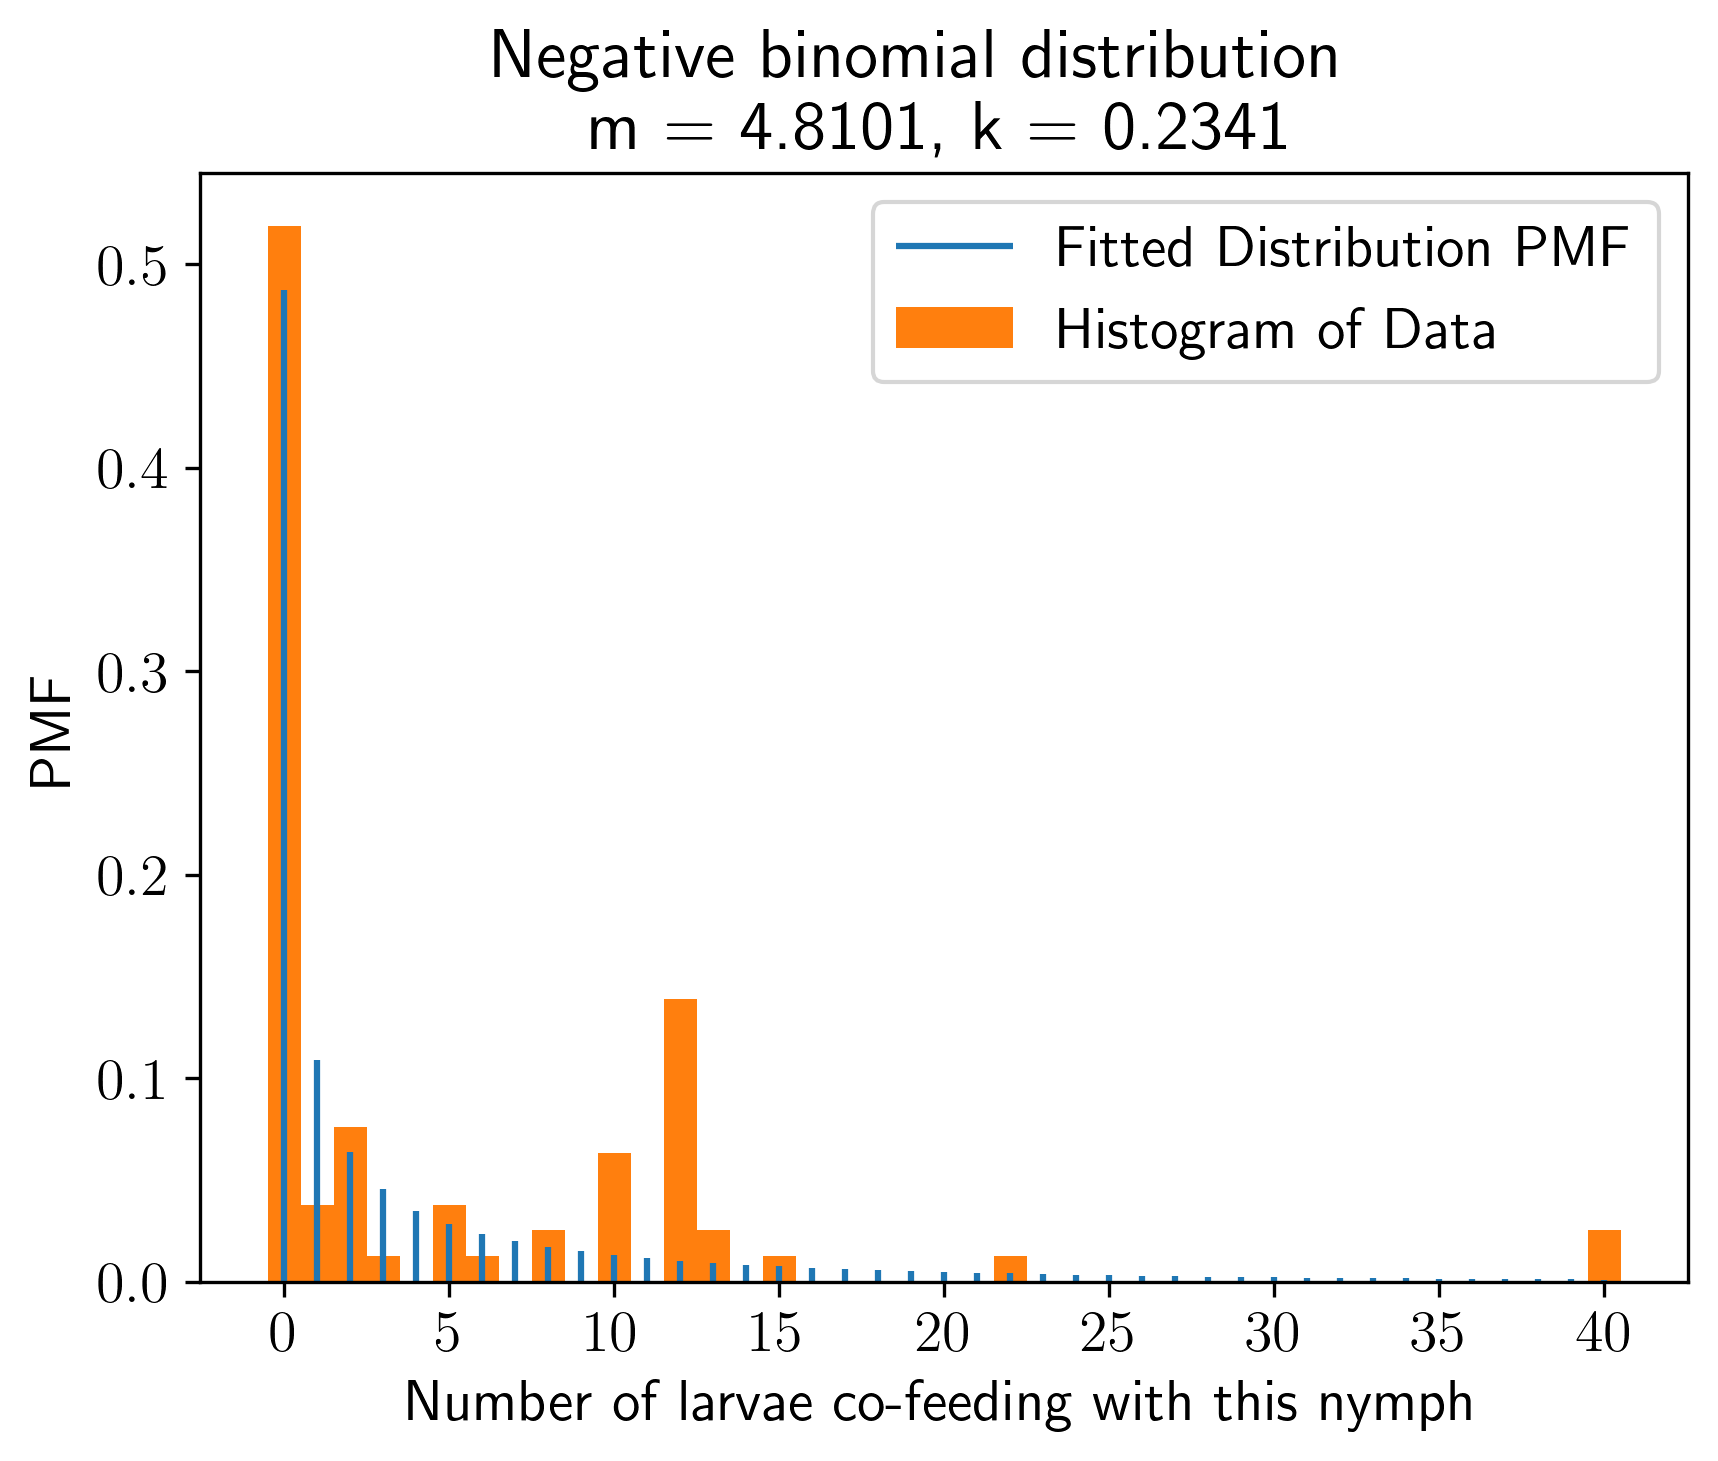
\includegraphics[width=0.5\textwidth, center]{coaggregation_dist_2005_I.trianguliceps_SA.png}
	\caption{For counts of \textit{I.trianguliceps} found on Common Shrews in 2005}\label{fig:distFit_2005_Itrianguliceps_SA}
	\end{mdframed}
\end{figure}

\clearpage

\subsection{Estimates for \texorpdfstring{$ \alpha $}{alpha} and its effect on \texorpdfstring{$ R_0 $}{R0}}

Now that we have estimates for the sample mean of the co-aggregation data $ X $, obtained from subsets of the Kielder Forest data, we could obtain a particular estimate for $ R_0 $ based on some $ \alpha $ that we calculate \eqref{alphaDef}. Researchers who wish to approximate the probability that a new outbreak becomes extinct would need to provide estimates about their particular tick species, host species, pathogen and environmental conditions.

However, we can understand the effect on $ R_0 $ without specifying the value of $ \alpha $ by utilising the simple linear equation \eqref{FindingR0FromCoaggregationMean}. Since a chain of transmission will certainly become extinct if $ R_0 \le 1 $, then we are interested in the case where $ R_0 > 1 $. In other words, what is the minimum value of $ \alpha $ such that a chain of transmissions might persist? This is found with:

\begin{equation}
	R_0 = m\alpha > 1 \implies \alpha > \frac{1}{m} \nonumber
\end{equation}

Since $ m $ is known for each subset of Kielder Forest data, then letting $ \alpha $ vary allows us to see the effect on $ R_0 $. The minimum values of $ \alpha $ that would allow for $ R_0 > 1 $, for each subset of the Kielder Forest data, are shown in Table \ref{tab:alpha_threshold}. Note that since $ 0 \le \alpha \le 1 $ then this imposes bounds on the value that $ R_0 $ can possibly take. Also, $ m < 1 \implies R_0 < 1 $, hence the N/A result in Table \ref{tab:alpha_threshold}.

\begin{table}[h]
	\begin{mdframed}[backgroundcolor=grey250,rightline=false,leftline=false,topline=false]
	\centering
	\begin{tabular}{|l|l|l|r|r|}
		\hline
		\textbf{Year} & \textbf{Tick species} & \textbf{Host species} & \multicolumn{1}{l|}{\textbf{$m$}} & \multicolumn{1}{l|}{\textbf{$ \alpha $ threshold}} \\ \hline
		2004          & \textit{I. ricinus}            & \textit{Common Shrew}          & 3.929                             & 0.255                                              \\ \hline
		2004          & \textit{I. trianguliceps}      & \textit{Common Shrew}         & 6.387                             & 0.157                                              \\ \hline
		2005          & \textit{I. ricinus}            & \textit{Field Vole}           & 14.75                             & 0.068                                              \\ \hline
		2005          & \textit{I. trianguliceps}      & \textit{Common Shrew}          & 4.81                              & 0.208                                              \\ \hline
		2005          & \textit{I. trianguliceps}      & \textit{Field Vole}            & 0.154                             & N/A                                                \\ \hline
	\end{tabular}
	\caption{This table presents the threshold that $ \alpha $ must surpass that would allow $ R_0 > 1 $.} 
	\label{tab:alpha_threshold}
	\end{mdframed}
\end{table}

\newpage

\section{Estimates for the probability that a chain of transmissions becomes extinct} 

Finally we can use estimates of $ k $ and $ R_0 $, obtained for each subset of Kielder Forest data, to approximate the probability that a chain of transmissions becomes extinct after the introduction of a single infectious tick. By using the negative binomial distribution's probability generating function \eqref{NegBinom_PGF}, reparameterised to use parameters $ R_0 $ and $ k $, we can use fixed point iteration to approximate the probability of eventual extinction. However, since we do not know the actual value of $ R_0 $, we instead graphically show the range of extinction probabilities based on the possible values of $ \alpha $.

We take inspiration from Figures \ref{fig:probabilityOfExtinction}, \ref{fig:firstGenerationToReach100Offspring}, which are reproduced to follow the example set by Lloyd-Smith et al \cite{LloydSmith2005}, to generate Figures \ref{fig:simulation_2004_iricinus_SA}, \ref{fig:simulation_2004_itrianguliceps_SA}, \ref{fig:simulation_2005_iricinus_FV}, \ref{fig:simulation_2005_itrianguliceps_SA}. We use the same methodology to generate both sets of figures, however, where $ R_0 $ and $ k $ vary in Figure \ref{fig:probabilityOfExtinction}, we will instead let $ \alpha $ vary for each subset of Kielder Forest data while we fix the value of $ k $, which is known. And where $ R_0=1.5 $ for different values of $ k $ in Figure \ref{fig:firstGenerationToReach100Offspring}, we will instead fix $ k $ for each subset of Kielder Forest data while allowing $ \alpha $ to vary in those simulations. In the simulation (right) chart of Figures \ref{fig:simulation_2004_iricinus_SA}, \ref{fig:simulation_2004_itrianguliceps_SA}, \ref{fig:simulation_2005_iricinus_FV}, \ref{fig:simulation_2005_itrianguliceps_SA}, we chose four equally-spaced values of $ \alpha $ between the minimum that would allow $ R_0 > 1 $ and $ \alpha=0.5 $. While values of $ \alpha > 0.5 $ are possible, there may be unknown factors that reduce the probability of a co-feeding larva becoming an infectious nymph. So, lower values of $ \alpha $ are assumed to be more realistic. 

In Figures \ref{fig:simulation_2004_iricinus_SA}, \ref{fig:simulation_2004_itrianguliceps_SA}, \ref{fig:simulation_2005_iricinus_FV}, \ref{fig:simulation_2005_itrianguliceps_SA} the minimum value of $ \alpha $ such that $ R_0 > 1 $ are displayed as broken vertical lines. Extinction with $ q=1 $ is guaranteed below those threshold values . The result of simulation (right in each figure) shows that for lower values of $ \alpha $, on average, there are more generations required before an outbreak reaches the benchmark defined by Lloyd-Smith et al. We also see lower rates of outbreaks surviving for lower values of $ \alpha $, which is expected.

The results of these simulations show varied outcomes. In Figure \ref{fig:simulation_2005_iricinus_FV} we can see a rapid decline of the extinction probability $ q $ for relatively low values of $ \alpha $, and relatively few generations before a generation with 100 offspring is found. In stark contrast, Figure \ref{fig:simulation_2005_itrianguliceps_SA} shows only a modest decline in $ q $ as $ \alpha $ increases, while many more generations on average are required before a generation with 100 offspring is found. The unsurprising result is that in some combinations of tick and host species, co-feeding in the absence of other forms of transmission is viable to maintain a pathogen in nature if a pathogen can have a sufficiently high $ \alpha $ (previously defined as the probability that a co-feeding larva becomes an infectious nymph). However, this is only part of the story.

\begin{figure}[]
	\begin{mdframed}[backgroundcolor=grey250,rightline=false,leftline=false,topline=false]
		\centering
		\begin{tabular}{ll}
			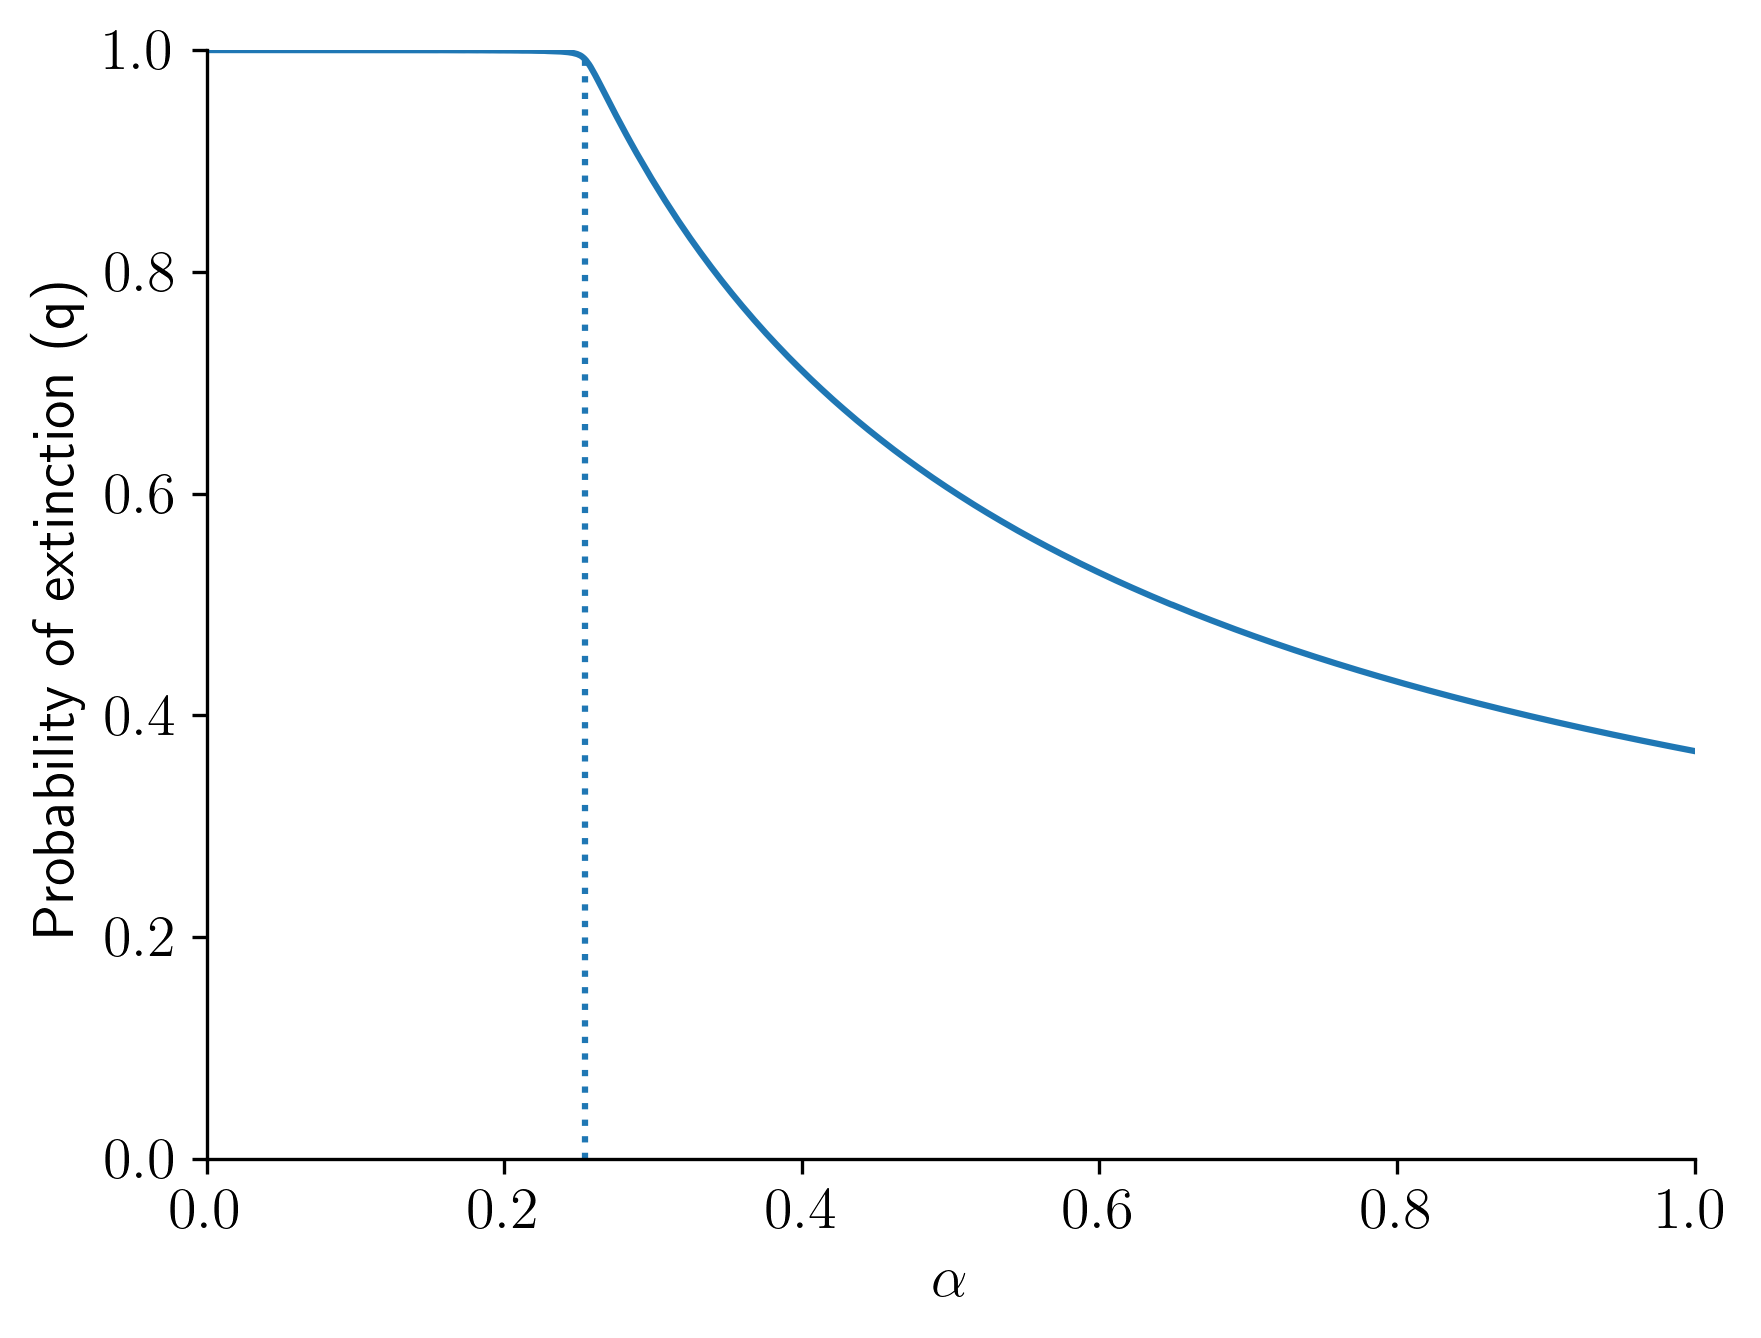
\includegraphics[width=.46\linewidth,valign=m]{extinctionProbability2004_I. ricinus_SA} & 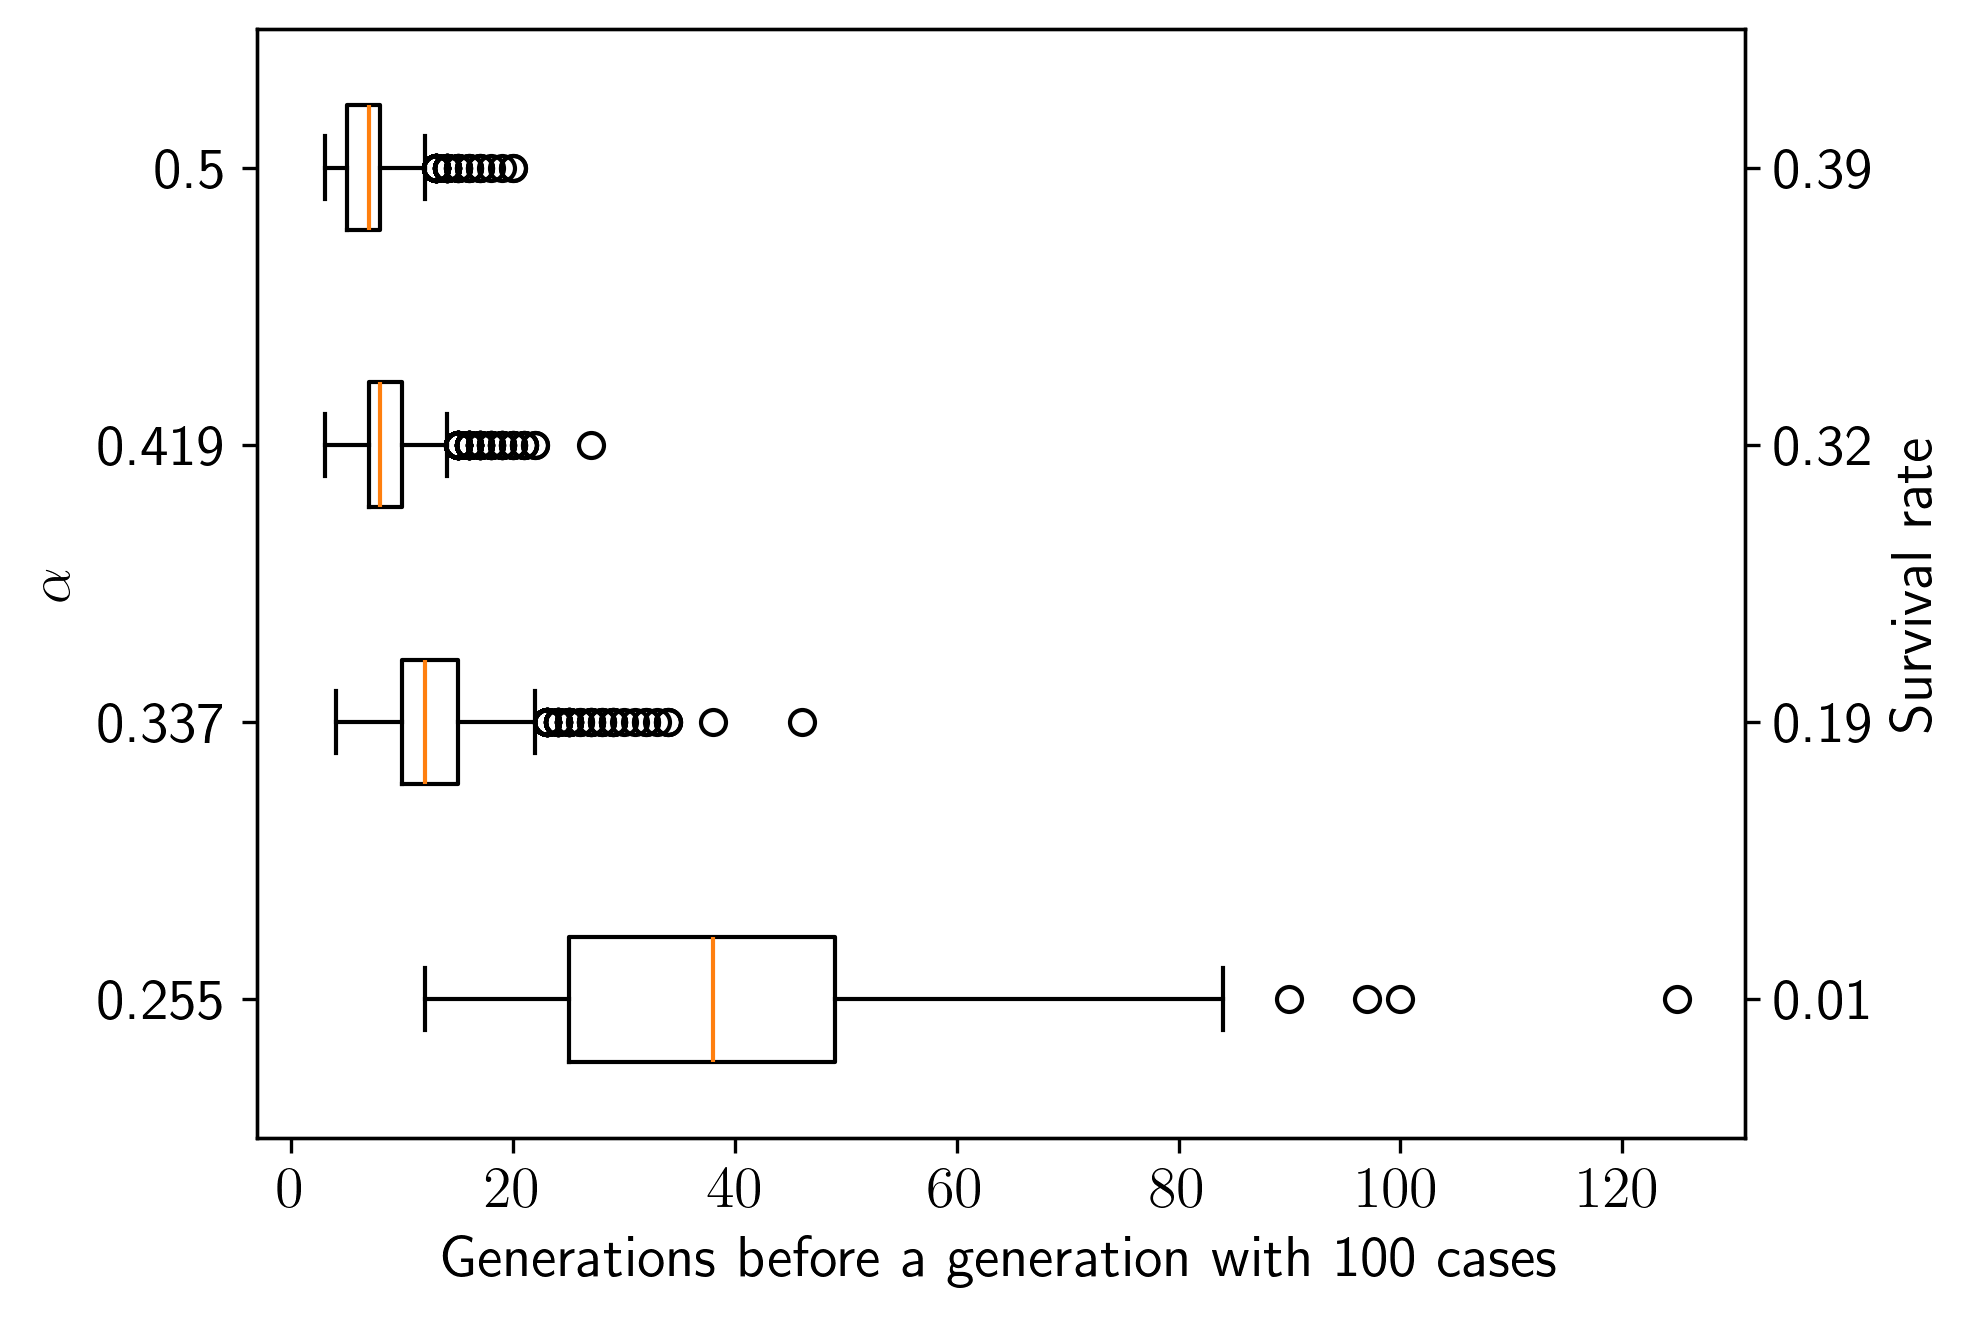
\includegraphics[width=.50\linewidth,valign=m]{firstGeneration100_2004_I. ricinus_SA}
		\end{tabular}
		\caption{(Left) probability of extinction depending on $ \alpha $ and (right) the number of generations to reach a generation with 100 offspring depending on $ \alpha $, and  outbreaks' survival rates after 10,000 generations, for \textit{I. ricinus} found on \textit{common shrews} in \textit{2004}, and where $ m = 3.939, k = 0.622 $ }
		\label{fig:simulation_2004_iricinus_SA}
	\end{mdframed}
\end{figure}

\begin{figure}[]
	\begin{mdframed}[backgroundcolor=grey250,rightline=false,leftline=false,topline=false]
		\centering
		\begin{tabular}{ll}
			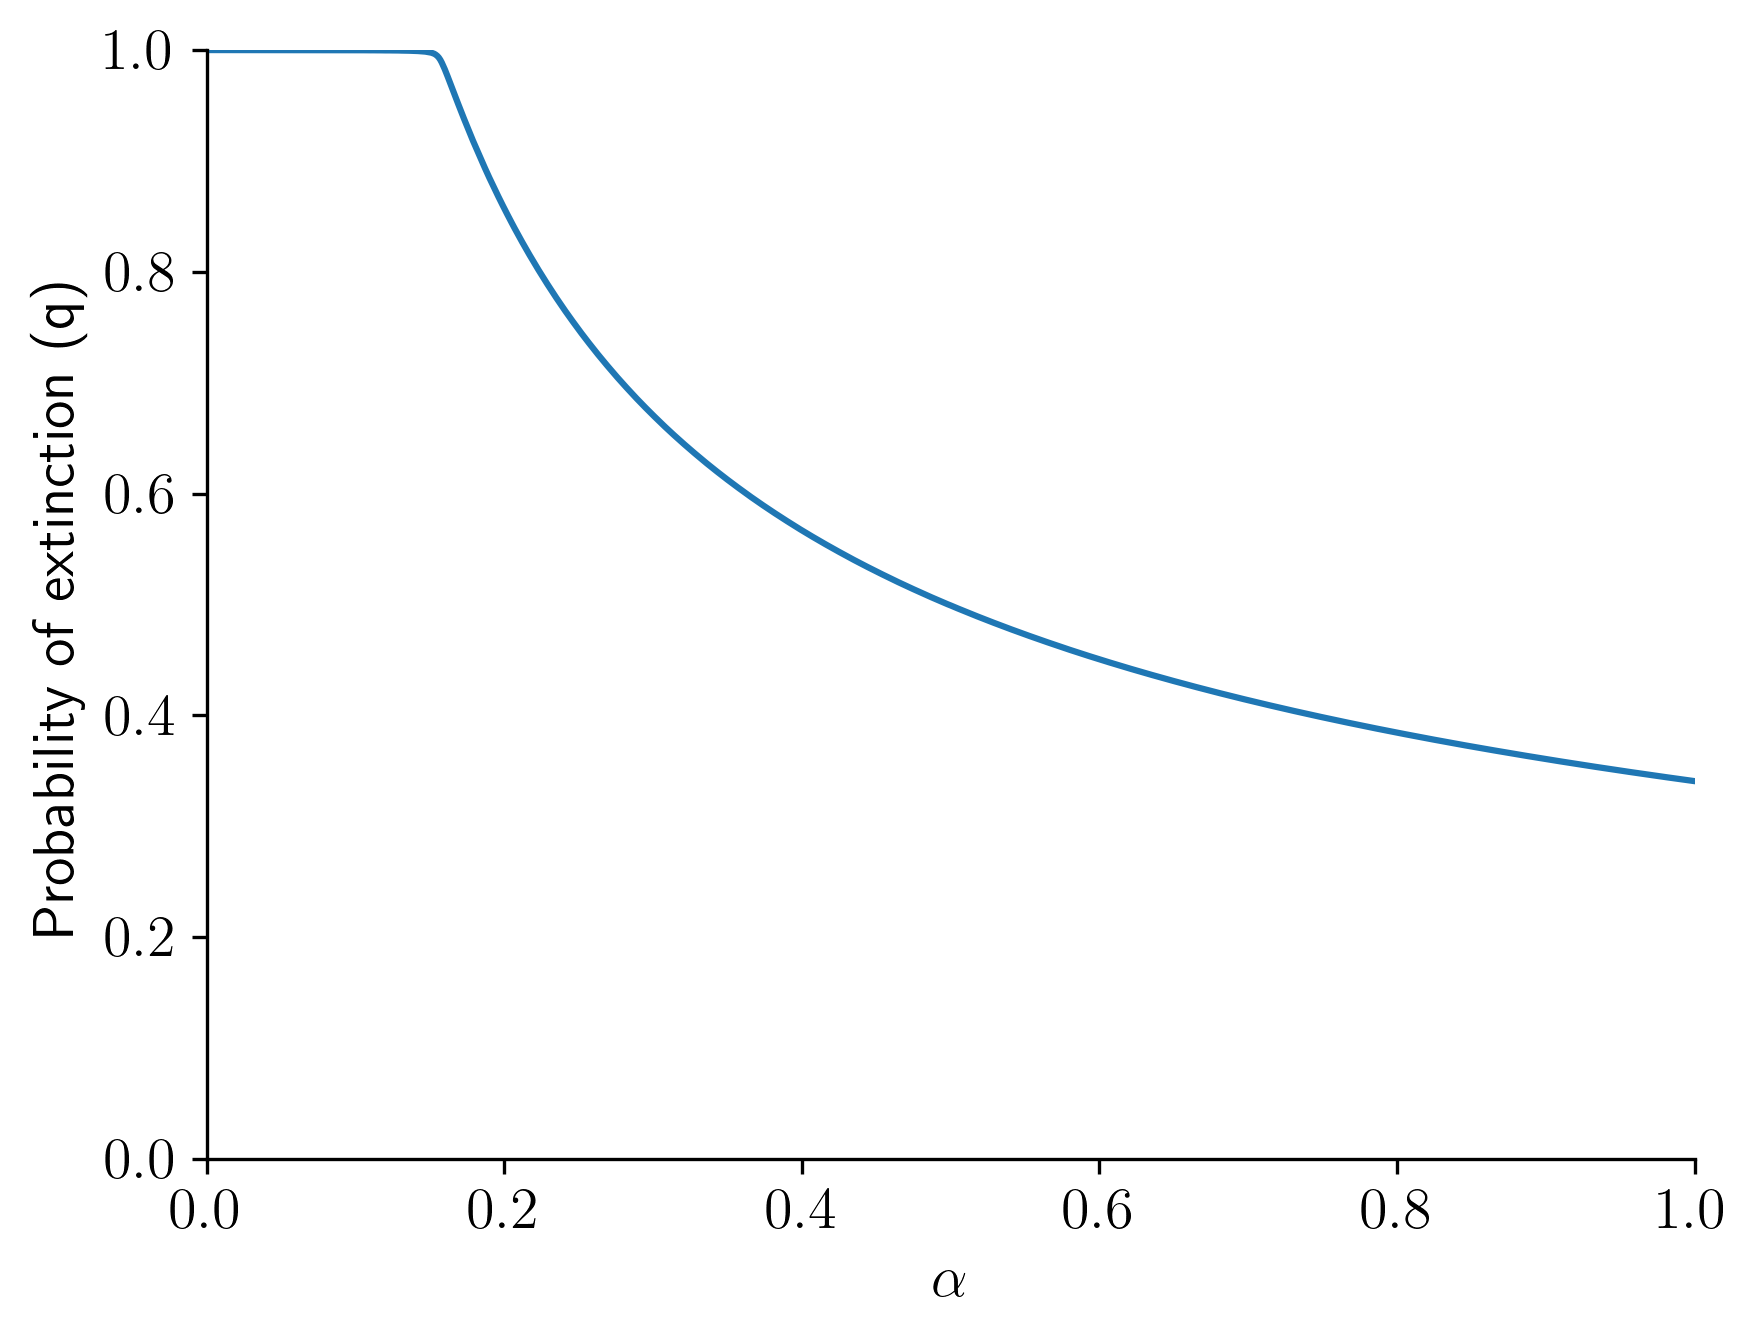
\includegraphics[width=.46\linewidth,valign=m]{extinctionProbability2004_I. trianguliceps_SA} & 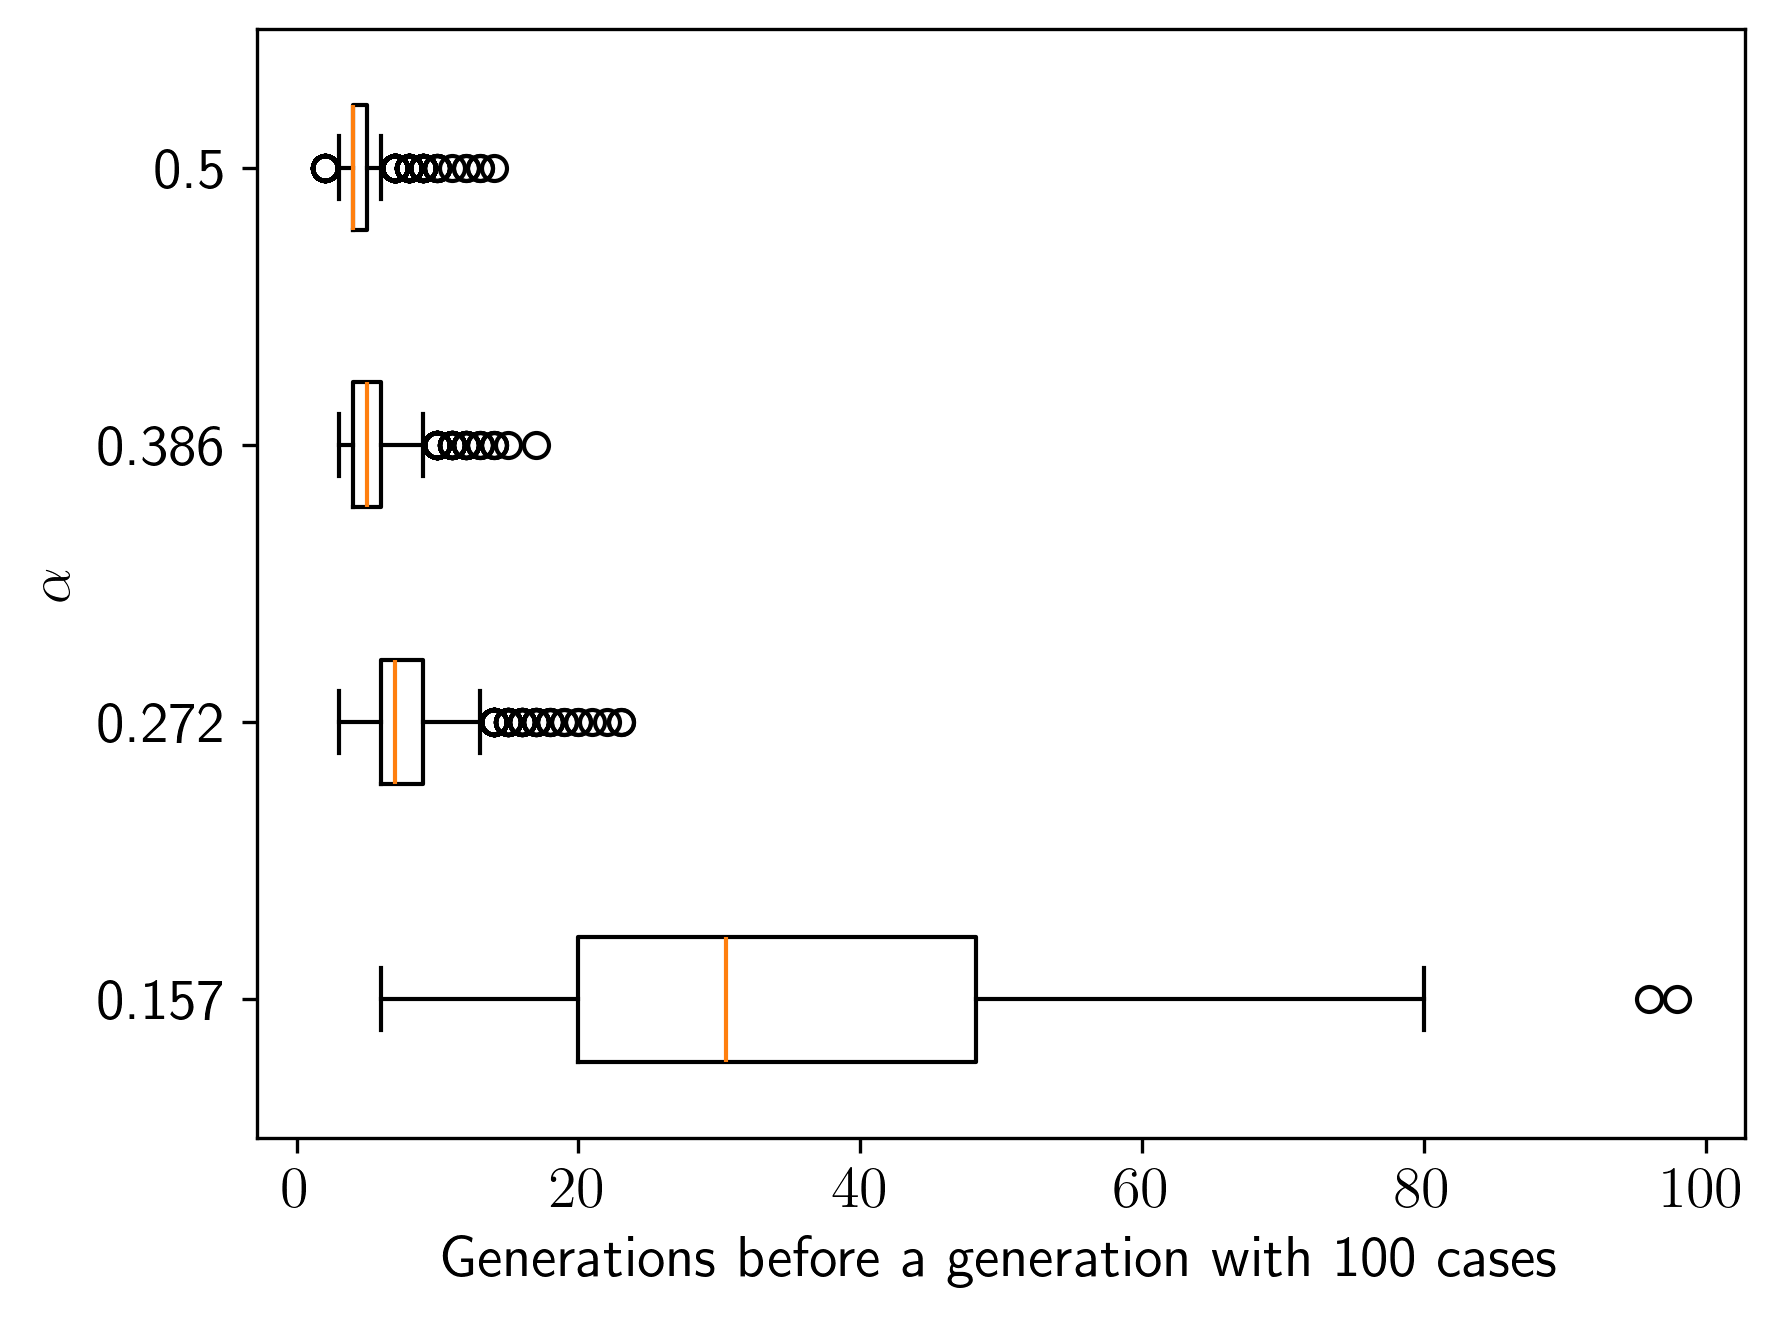
\includegraphics[width=.50\linewidth,valign=m]{firstGeneration100_2004_I. trianguliceps_SA}
		\end{tabular}
		\caption{(Left) probability of extinction depending on $ \alpha $ and (right) the number of generations to reach a generation with 100 offspring depending on $ \alpha $, and  outbreaks' survival rates after 10,000 generations, for \textit{I. trianguliceps} found on \textit{common shrews} in \textit{2004}, and where $ m = 6.387, k = 0.478 $. }
		\label{fig:simulation_2004_itrianguliceps_SA}
	\end{mdframed}
\end{figure}

\begin{figure}[]
	\begin{mdframed}[backgroundcolor=grey250,rightline=false,leftline=false,topline=false]
		\centering
		\begin{tabular}{ll}
			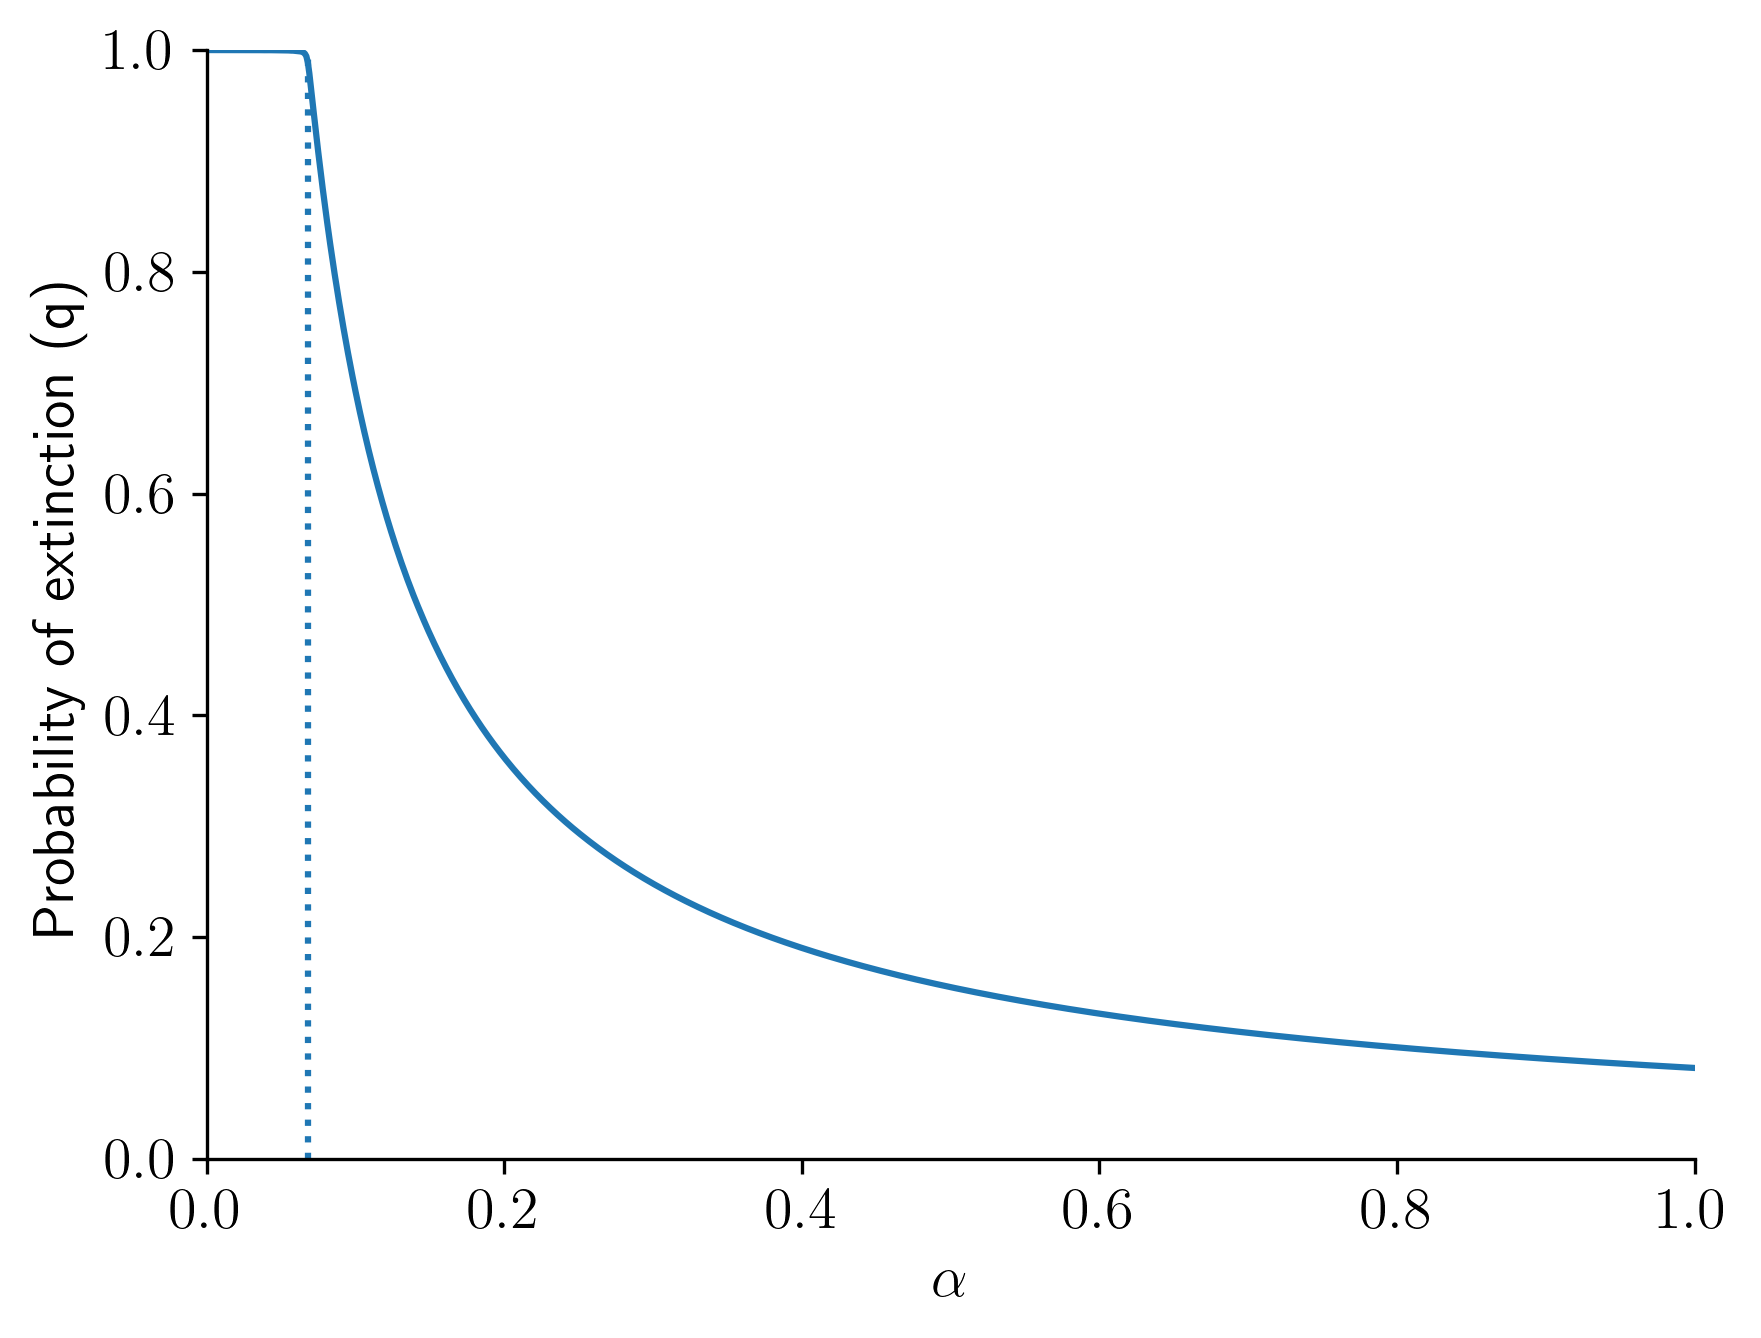
\includegraphics[width=.46\linewidth,valign=m]{extinctionProbability2005_I. ricinus_FV} & 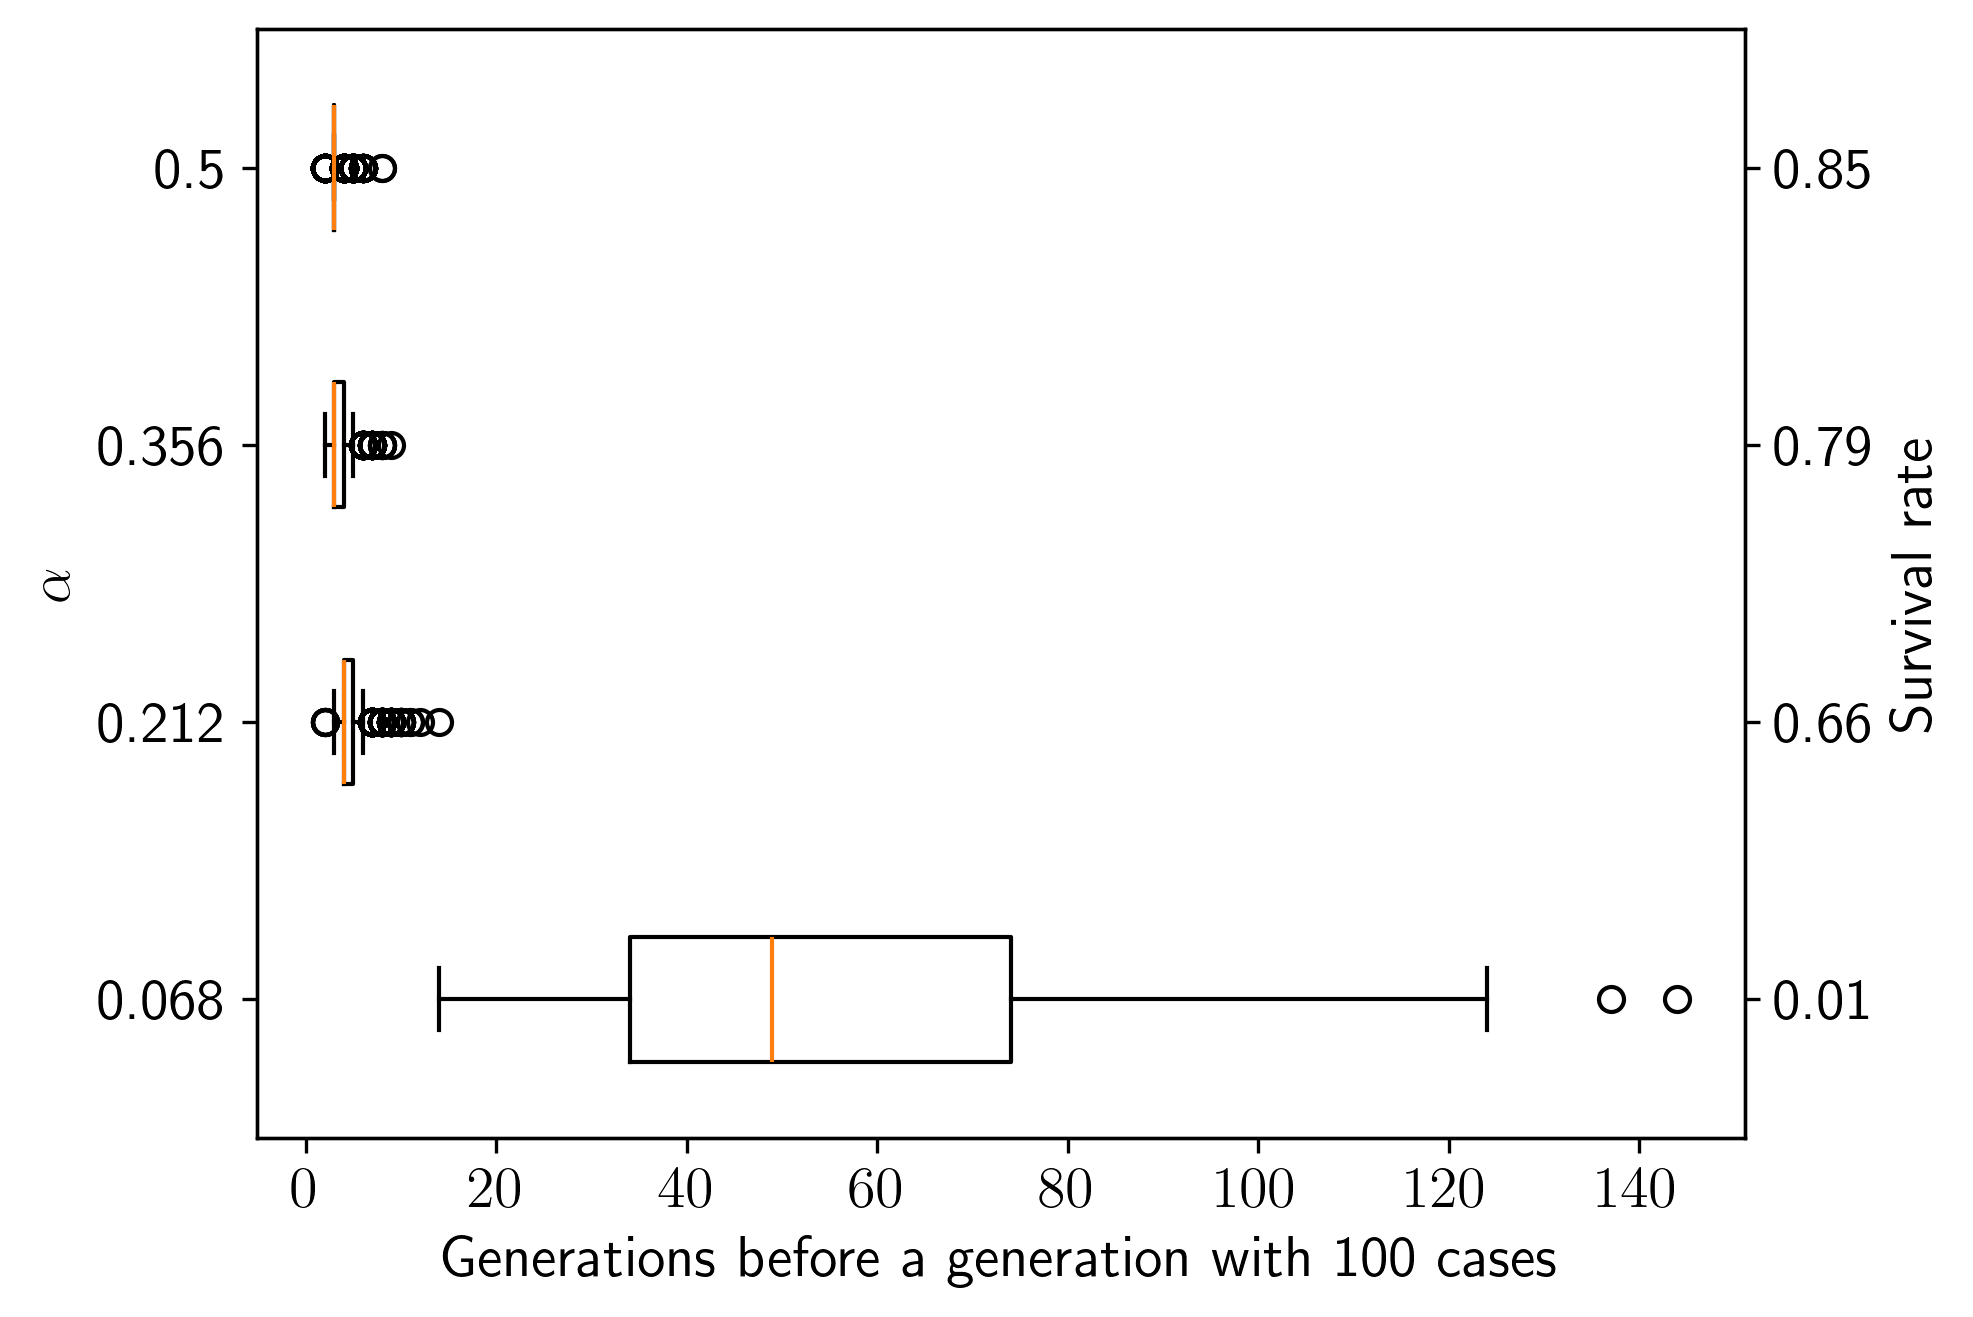
\includegraphics[width=.50\linewidth,valign=m]{firstGeneration100_2005_I. ricinus_FV}
		\end{tabular}
		\caption{(Left) probability of extinction depending on $ \alpha $ and (right) the number of generations to reach a generation with 100 offspring depending on $ \alpha $, and  outbreaks' survival rates after 10,000 generations, for \textit{I. ricinus} found on \textit{field voles} in \textit{2005}, and where $ m = 14.75, k = 0.9019 $.}
		\label{fig:simulation_2005_iricinus_FV}
	\end{mdframed}
\end{figure}

\begin{figure}[]
	\begin{mdframed}[backgroundcolor=grey250,rightline=false,leftline=false,topline=false]
		\centering
		\begin{tabular}{ll}
			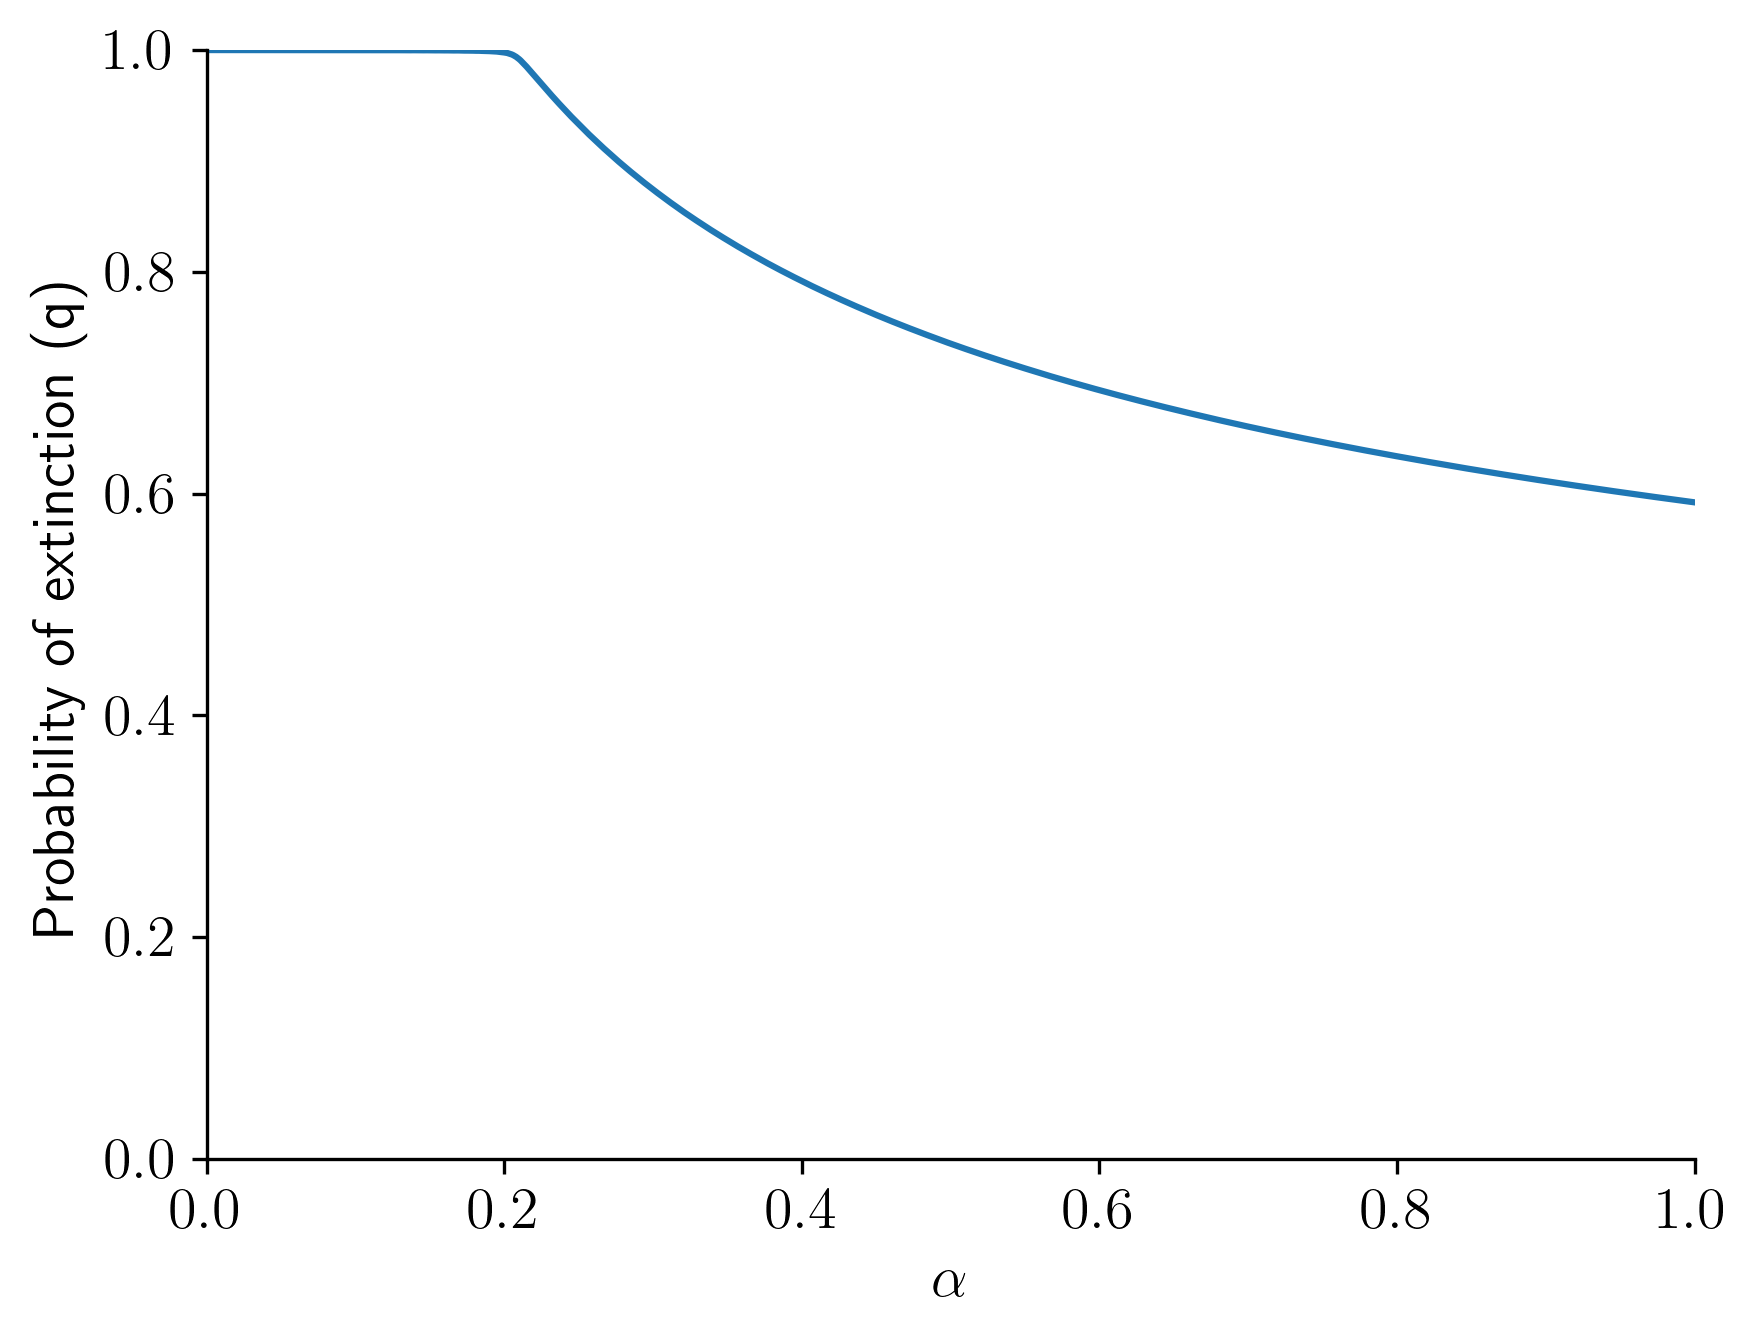
\includegraphics[width=.46\linewidth,valign=m]{extinctionProbability2005_I. trianguliceps_SA} & 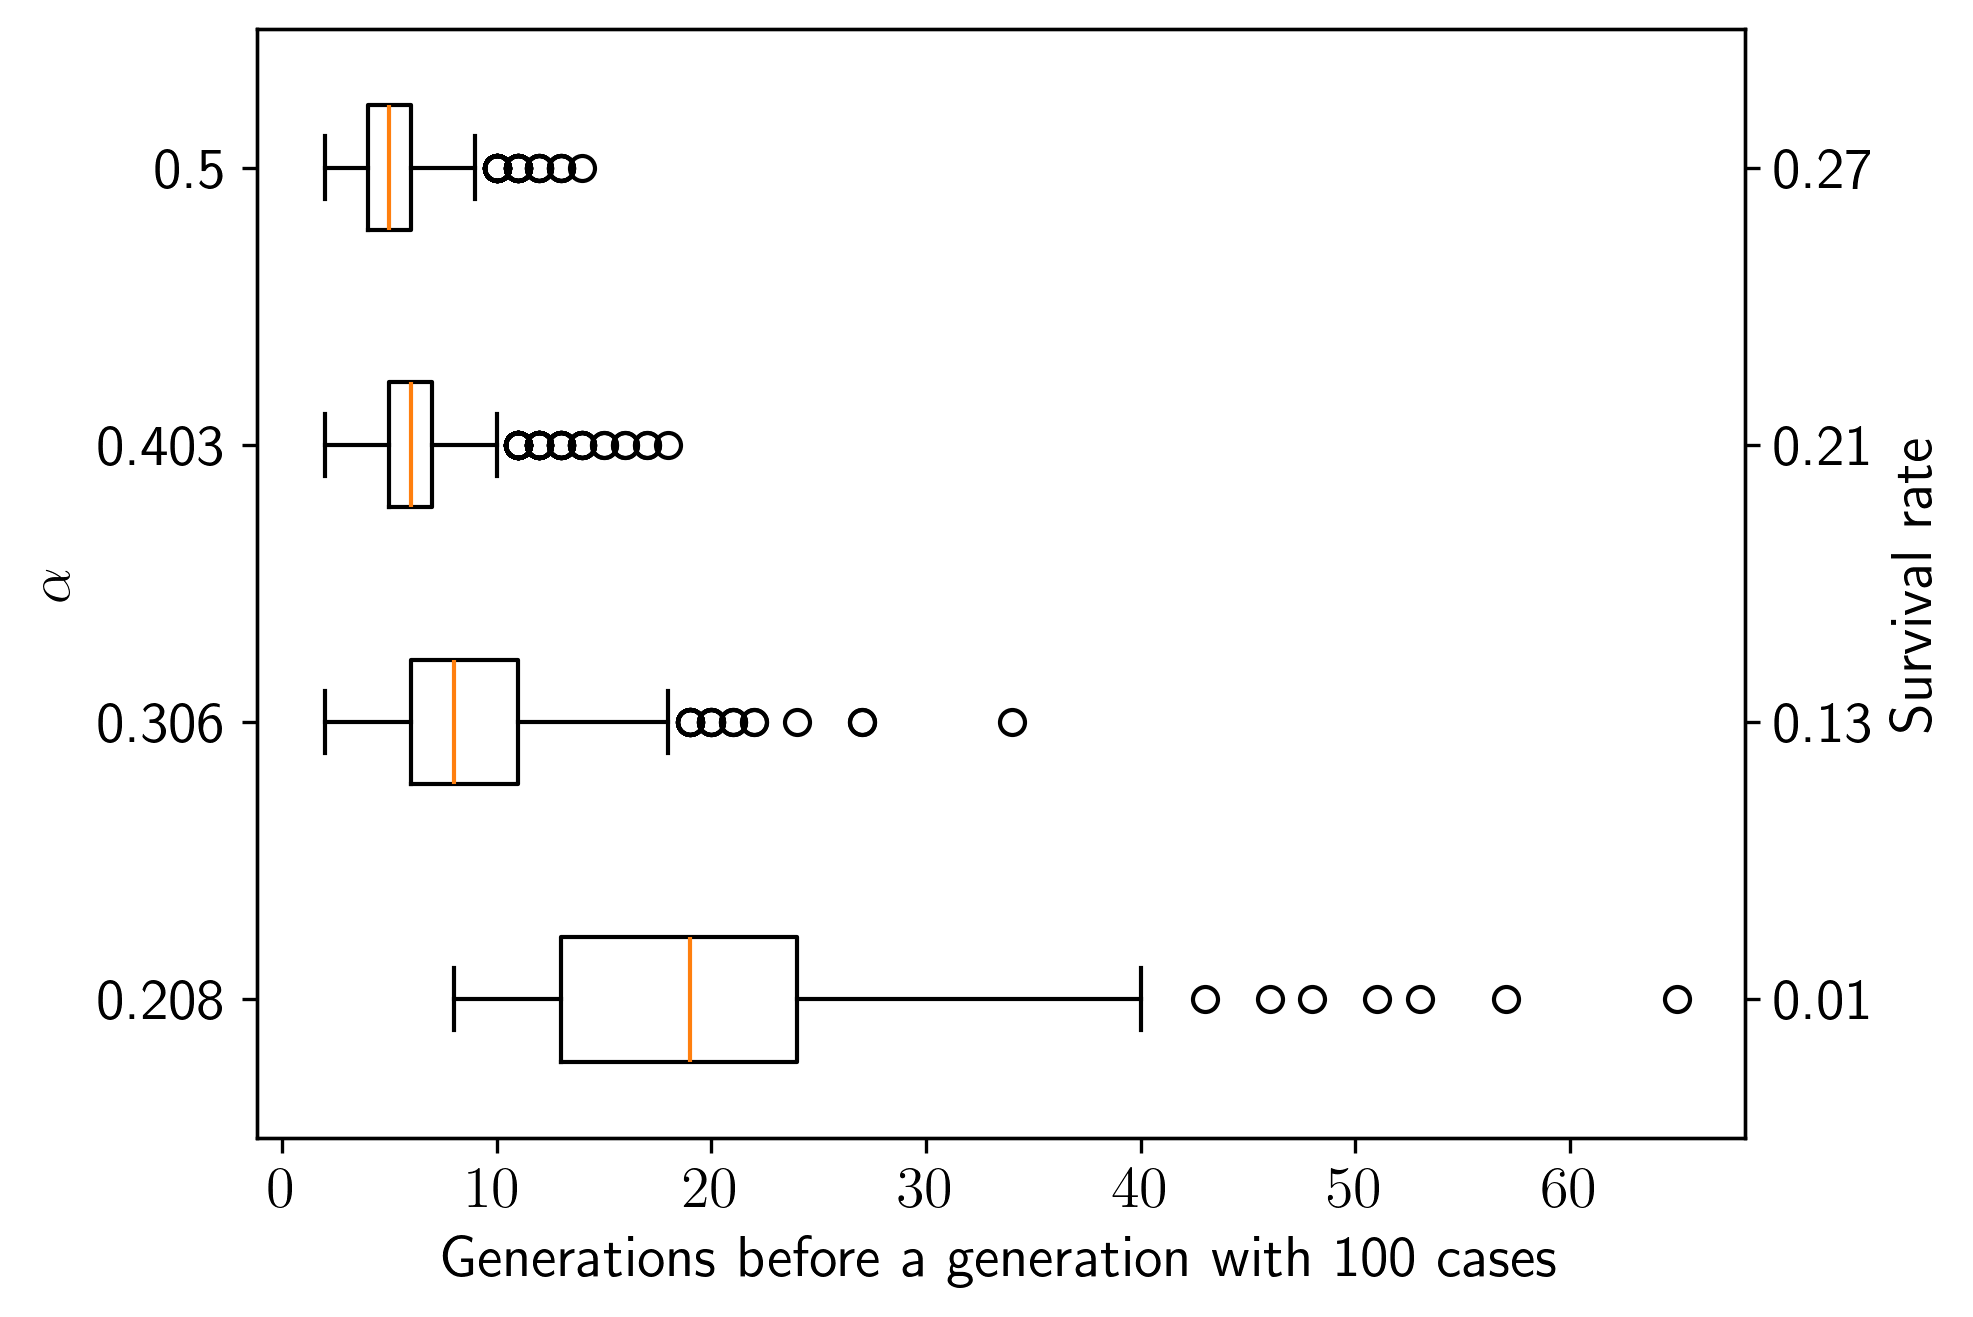
\includegraphics[width=.50\linewidth,valign=m]{firstGeneration100_2005_I. trianguliceps_SA}
		\end{tabular}
		\caption{(Left) probability of extinction depending on $ \alpha $ and (right) the number of generations to reach a generation with 100 offspring depending on $ \alpha $, and  outbreaks' survival rates after 10,000 generations, for \textit{I. trianguliceps} found on \textit{common shrews} in \textit{2005}, and where $ m = 4.81, k = 0.234 $.}
		\label{fig:simulation_2005_itrianguliceps_SA}
	\end{mdframed}
\end{figure}

To see the effect of $ k $ in each subset of Kielder Forest data, we can instead assume that each subset has an offspring distribution with $ R_0 = 1.5 $. Figure \ref{fig:allCombinations_firstGenerationReach100Offspring} is a re-implementation of Figure \ref{fig:firstGenerationToReach100Offspring}, using exactly the same methodology, but instead of using arbitrarily-chosen values of $ k $ we will use the values of $ k $ found by fitting the negative binomial distribution to each subset of Kielder Forest data. Figure \ref{fig:allCombinations_populationsOfOutbreaksThatWentExtinct} is another iteration of the same simulation that also uses the fitted values of $ k $, but instead shows the total population of outbreaks that became extinct. Taken together, Figures \ref{fig:allCombinations_firstGenerationReach100Offspring}, \ref{fig:allCombinations_populationsOfOutbreaksThatWentExtinct} reveal that if these particular combinations of tick and host species involved a pathogen, or pathogens, that could infect larvae at a rate of $ R_0 = 1.5 $ per infectious nymph, then those combinations that have lower $ k $ will on average reach the arbitrary benchmark in fewer generations. Outbreaks that become extinct will have roughly the same populations on average, but the outbreaks that have a lower $ k $ but will include more extreme values. This shows the influence of superspreading: some nymphs co-feed with a disproportionately high number of larvae, leading to explosive growth that still sometimes ends with eventual extinction.

\begin{figure}[]
	\begin{mdframed}[backgroundcolor=grey250,rightline=false,leftline=false,topline=false]
		\centering
		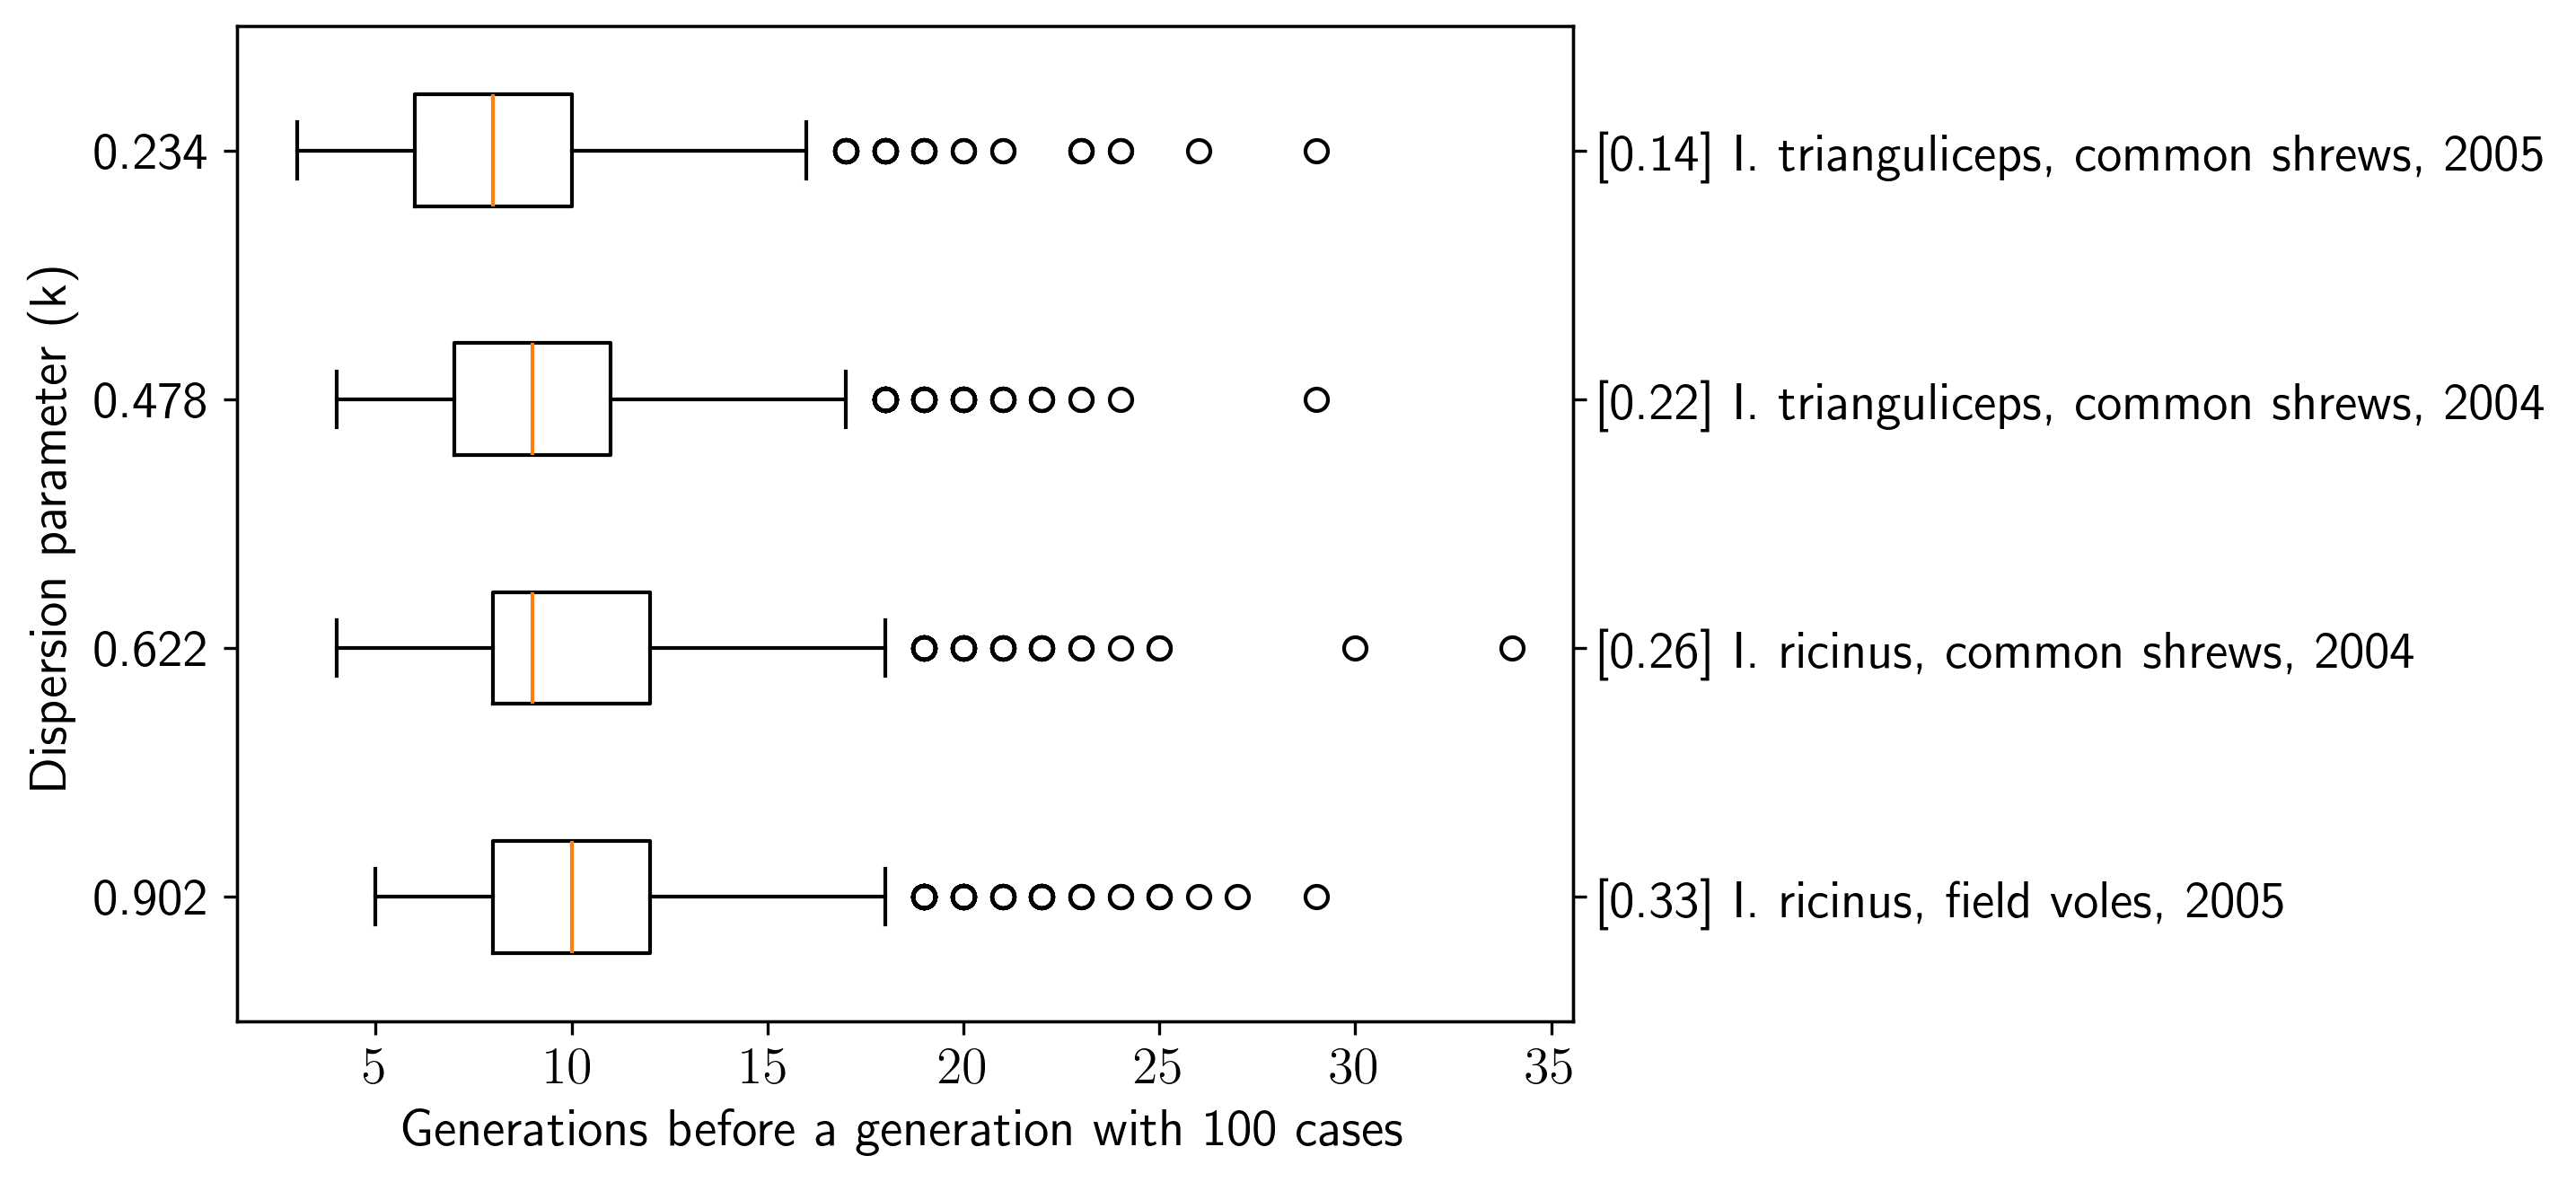
\includegraphics[width=.73\linewidth,valign=m]{allCombinations_firstGenerationReach100Offspring}
		\caption{The number of generations to reach a generation with 100 offspring depending on $ k $, where $ R_0 = 1.5 $, for all combinations of Kielder Forest data that have $ m \ge 1 $. The values in square brackets are outbreaks' survival rates after 10,000 generations.}
		\label{fig:allCombinations_firstGenerationReach100Offspring}
	\end{mdframed}
\end{figure}

\begin{figure}[]
	\begin{mdframed}[backgroundcolor=grey250,rightline=false,leftline=false,topline=false]
		\centering
		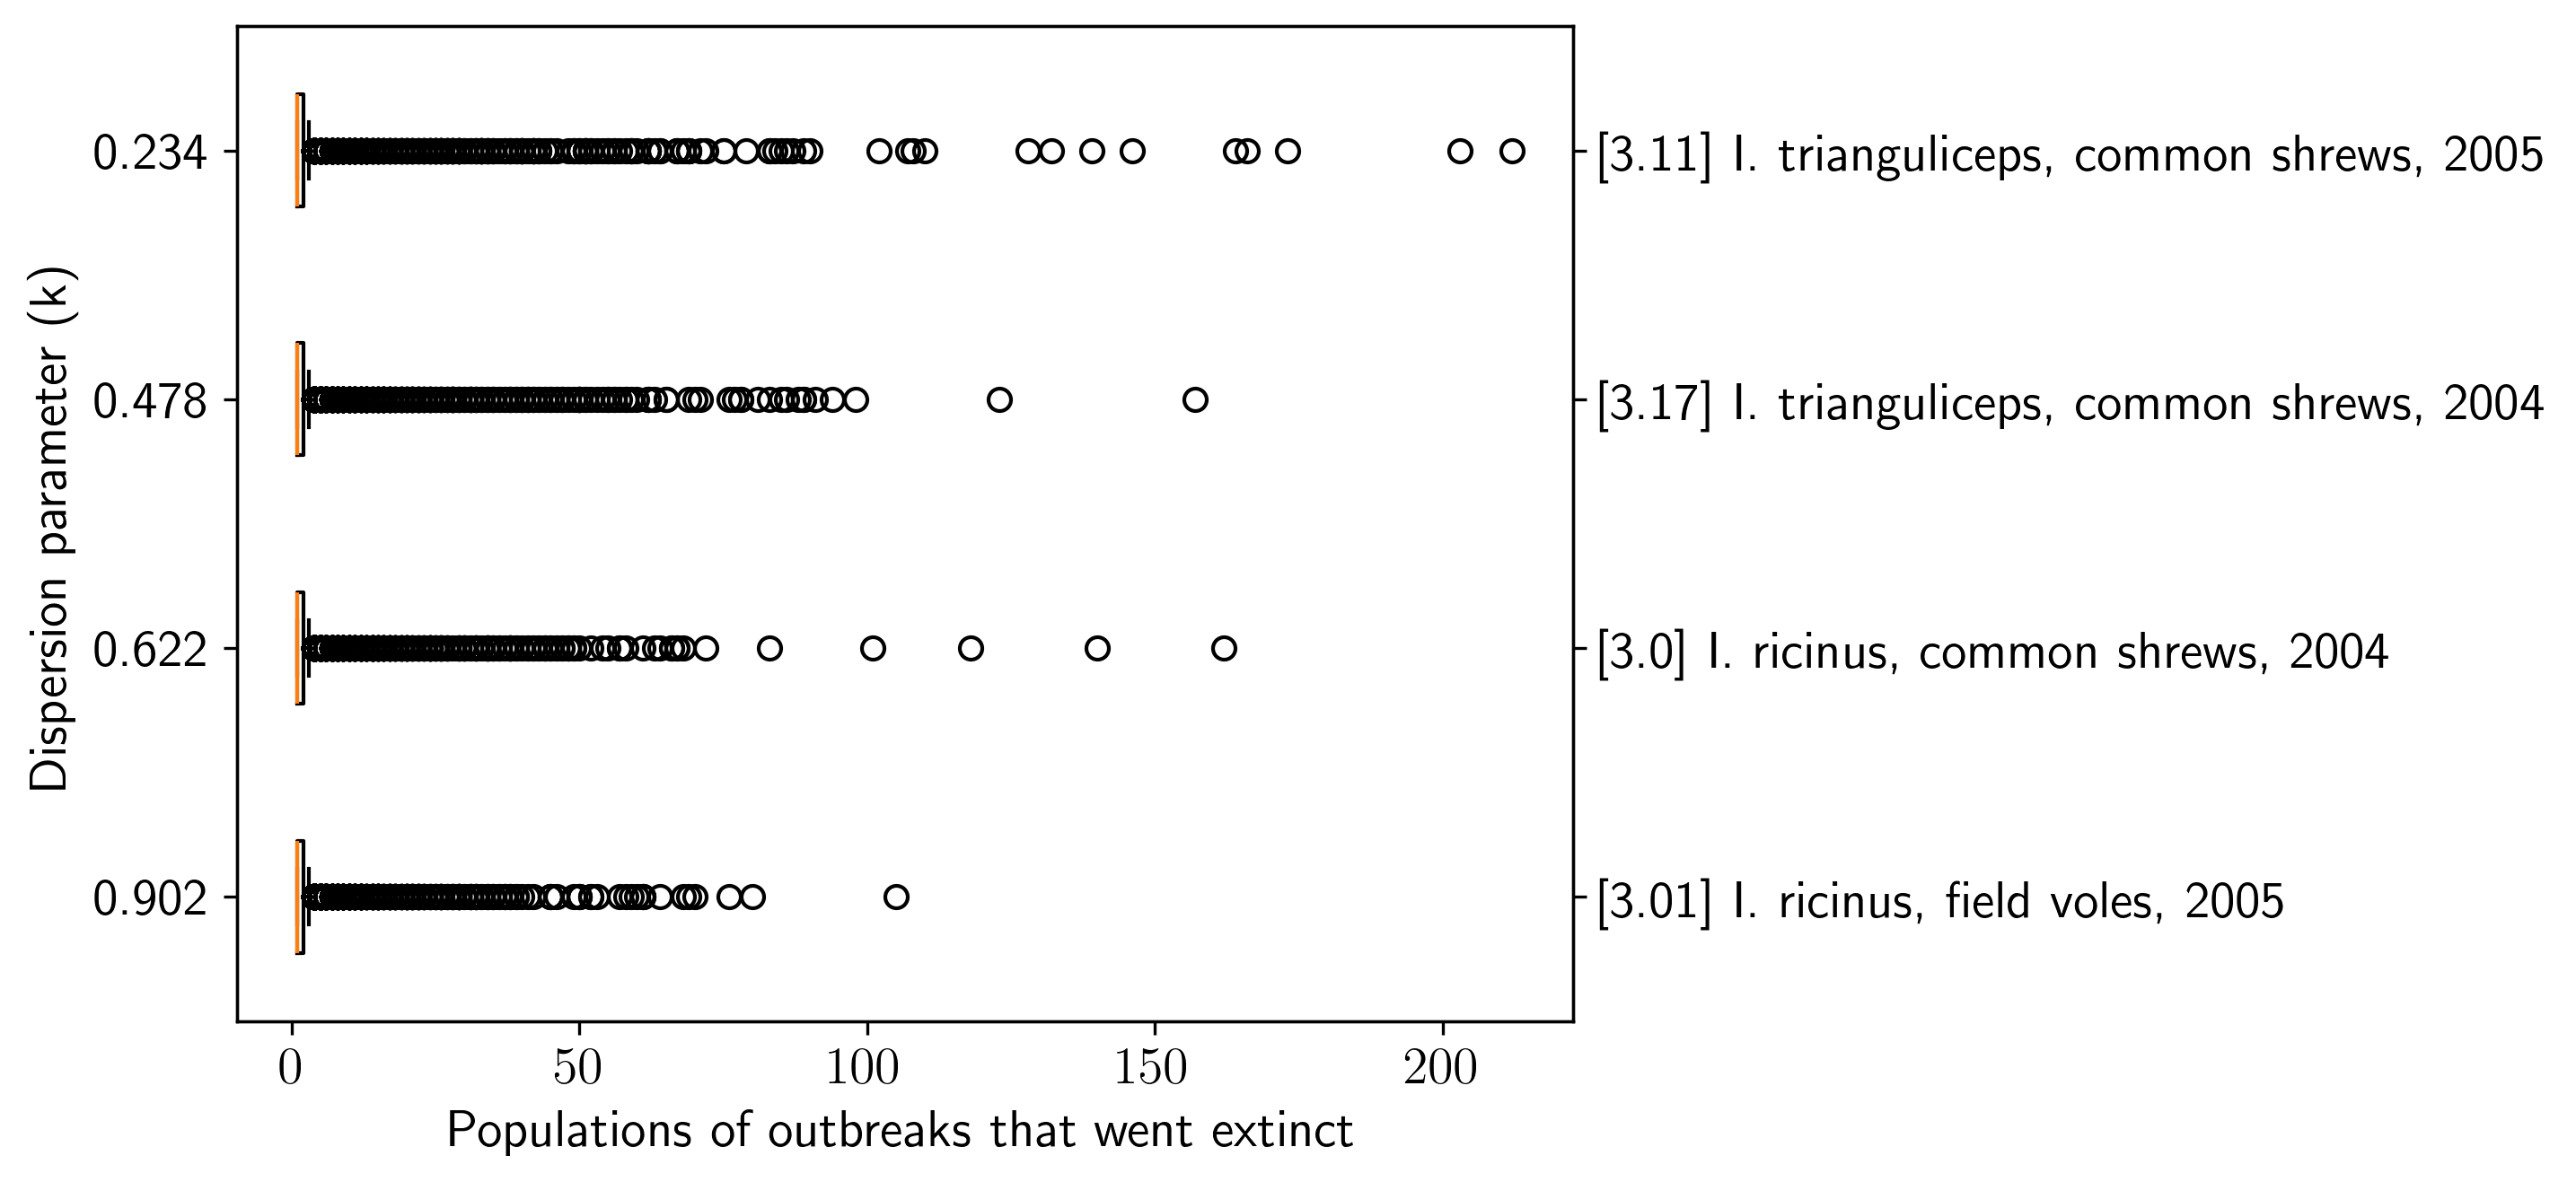
\includegraphics[width=.73\linewidth,valign=m]{allCombinations_populationsOfOutbreaksThatWentExtinct}
		\caption{The total populations of outbreaks that became extinct where $ R_0 = 1.5 $, for all combinations of Kielder Forest data that have $ m \ge 1 $. The values in square brackets are mean outbreaks population.}
		\label{fig:allCombinations_populationsOfOutbreaksThatWentExtinct}
	\end{mdframed}
\end{figure}

\clearpage
\newpage

\section{Discussion}

In this project we have made assumptions that vary in the reason for their introduction; some are simplifying assumptions that make the task more tractable, while some are appropriate due to the biological realism we wish to emulate. This discussion will focus on the assumptions made and the consequences of using those. We will also consider alternative assumptions we could have used, and potential ideas for future research based on modified assumptions.

The first and most obvious assumption in this project was to make co-feeding transmission the only viable route of transmission. This assumption is of interest since various factors are causing ticks to spread \cite{} and therefore, it is possible that a tick carrying some pathogen might move into an area where a naive population of vertebrate hosts are incompetent to maintain that pathogen. In that case, the role of systemic transmission would be limited. Assuming that co-feeding is the only viable route of transmission also allows us to use a single-type GWBP, which is effective for understanding the risk of extinction at the start of an outbreak for a directly-transmissible pathogen \cite{}, but only when every new offspring is the same type and with the same offspring distribution for the entire analysis. Only considering co-feeding transmission would of course be inappropriate for estimating the probability of extinction for many TBD systems, where we know systemic transmission is important. However even in those cases, it would still be interesting to find that some pathogens could exist with some combinations of tick and host species by co-feeding transmission alone.

The assumption that co-feeding transmission is from infectious nymph to a co-feeding larvae only is a simplifying assumption; in reality it is possible that an infected nymph will feed close to, and infect, other nymphs or even adult ticks. The Kielder Forest data, for example, has many recorded observations of captured vertebrates that each have multiple nymphs of the same species. But if we suppose that an infectious nymph did infect another nymph, then the newly-infected nymph would have to survive moulting before it could feed on another vertebrate host as an adult, which would most-likely be a large vertebrate host \cite{}. Given that the more-numerous immature ticks feed on smaller vertebrate hosts \cite{}, then that particular adult tick would be unlikely to co-feed with other ticks and that particular chain of transmissions would most likely end there.

We also make the simplifying assumption that more than one larvae that become infected in the same chain of transmissions will then co-feed as infectious nymphs on different vertebrate hosts. This is reasonable for non-nidicolous tick species, which tend to drop off their vertebrate hosts and moult in a wider range of locations \cite{}. Nidicolous ticks, however, tend to WHAT \cite{}. An alternative assumption would have been for multiple larvae to become infected and then to co-feed with other infectious nymphs on the same vertebrate host, as we might expect with nidicolous ticks. The effect of this might be to increase the overall probability $ \alpha $ \eqref{alphaDef} that co-feeding larvae become infected, due to more infectious nymphs increasing the overall load of pathogens. Alternatively, this situation could also be handled by dividing the co-feeding larvae amongst the infectious nymphs before applying $ \alpha $, in the sense that a co-feeding larva can become infected once.

The division of the Kielder Forest data into subsets that are each a combination of tick species, host species and year of capture has implications for how we can interpret the estimates of $ R_0, k $ and the probability that a chain of transmissions becomes extinct. The data is segregated by tick species, because the tick species under study, \textit{I. ricinus} and \textit{I. trianguliceps}, are not known to be vectors for the same pathogens \cite{}. Therefore, a larva that co-feeds with an infectious nymph of a different species will not become an infectious nymph with the same pathogen. Even if the two tick species under study were vectors for the same pathogen, then $ \alpha $ (the probability of a co-feeding larva becoming an infectious nymph) for each species would be different due to different moulting success rates and different magnitudes of vector competence.

This project also divided the Kielder Forest data into subsets by host species. This reflects that the probability of transmission for a single species of tick is different depending on which vertebrate host they feed on. The probability that ticks co-feed close enough for transmission to occur depends on the host species on which they feed; since the Field Vole is smaller than the Common Shrew, then we can expect different rates of transmission success during co-feeding for the two different species of host. However, partitioning the data by host species means the co-aggregation distribution leads to a loss of information; for example an infectious nymph could infect a larvae of the same species while co-feeding on a Common Shrew, and then, that larvae could survive to become a infectious nymph and co-feed with larvae of the same species on a Field Vole. Potentially, this could be addressed with a multi-type GWBP. That was outside the scope of this project, but would be interesting future research.

Some work is required by anyone who wishes to use the results of this research; calculating the probability of extinction in a TBD transmission network requires multiple steps. Firstly, once field data is obtained, it should be simple to count the number of larvae that co-feed with each nymph, from which one can obtain the sample mean for the co-aggregation data. Then, one can fit the reparameterised negative binomial distribution to obtain the dispersion parameter $ k $. The real work would be determining a viable estimate of $ \alpha $ \eqref{alphaDef}, which is needed to determine $ R_0 $. This would likely depend on the tick species, pathogen, host species and environmental conditions in which the transmission takes place. In this project, we were not able to determine accurate estimates for $ \alpha $, so instead we analysed what effect $ \alpha $ has on $ R_0 $ during co-feeding transmission. If one was to obtain plausible and reliable estimates for $ \alpha $, then $ R_0 $ due to co-feeding transmission could easily be obtained by using \eqref{FindingR0FromCoaggregationMean}.

\newpage

\section{Conclusion}

This project has investigated a scenario where co-feeding transmission is the only viable route of transmission for a tick-borne pathogen. We specifically looked at \textit{Ixodidae} (hard-bodied) ticks, which feed only once per life stage \cite{}. The project aim was to use a GWBP to find an approximate probability that a chain of transmissions becomes extinct, which is of particular interest at the start of an outbreak.

The analysis presented here indicates that for Kielder Forest, and for some combinations ot tick and host species, there may be cases where co-feeding transmission alone is viable to maintain a pathogen in nature. However it would require further work to determine the probability that a co-feeding larva becomes an infectious nymph, which we have called $ \alpha $, for a particular combination of tick, host and pathogen. The discussion reviews the many assumptions made and indicates that using a multi-type GWBP would be a good opportunity for future research.

\newpage

\section{References}
\printbibliography[heading=none]

\newpage

\section{Appendix}

The author completed all analysis using Python and Jupyter notebooks, and compiled this document using LaTeX (TeXstudio). All analysis, code, and LaTeX source files are available at \url{https://github.com/JasonThomasData/honours_project}.

Figures \ref{fig:graphical_abstract}, \ref{fig:coaggregation_diagram} were made using \url{https://app.diagrams.net/}.

Tables were formatted with \url{https://www.tablesgenerator.com/#}.


\end{document}